%2345678901234567890123456789012345678901234567890123456789012345678901234567890
%%%%%%%%%%%%%%%%%%%%%%%%%%%%%%%%%%%%%%%%%%%%%%%%%%%
% MAURICIO ESGUERRA NEIRA
% Ph. D. Thesis
%%%%%%%%%%%%%%%%%%%%%%%%%%%%%%%%%%%%%%%%%%%%%%%%%%%
% Need ruproposal.cls which formats to Rutgers Style Guide
\documentclass[11pt, oneside, pdftex]{ruformat}
\renewcommand{\thefootnote}{\roman{footnote}}
\usepackage{amsmath, amstext, amsfonts, amssymb}
\usepackage[pdftex]{graphicx}
\usepackage{subfigure, longtable}
\usepackage{float}
\usepackage{rotating}
%\restylefloat{figure}
\usepackage{longtable}
\usepackage{url}
%\usepackage{xtab}
\usepackage{setspace}
\usepackage{pdflscape}
\usepackage{threeparttable}
%\singlespacing
%The geometry package might not be necessary since there are definitions in
%ruformat.cls
\usepackage[left=2.54cm,bottom=2.00cm,top=2.00cm,right=2.54cm]{geometry}
%\usepackage[left=1.5in,bottom=1in,top=1in,right=1in]{geometry}
\usepackage{chapterbib}
\usepackage{makeidx}
\makeindex
%\includeonly{Chapter4/chapter4, Appendix/appendix4a}
\includeonly{titles, Chapter1/chapter1, Chapter2/chapter2,
  Chapter3/chapter3, Chapter4/chapter4, Appendix/appendix1a,
  Appendix/appendix2a, Appendix/appendix4a, Supplement/supplements}
%\usepackage{pdflscape}
\usepackage{hyperref}  %%Note: In TeXShop hyperref needs to be at the end of package calls.


%%%%%%%%%%%%%%%%%%%%%%%%%%%%%%%%%%%%%%%%%%%%%%%%%%%
%% Fonts in Document
%%%%%%%%%%%%%%%%%%%%%%%%%%%%%%%%%%%%%%%%%%%%%%%%%%%
%\usepackage{times}
%\usepackage{pslatex}
%\usepackage{newcent}
%\usepackage{palatcm}
%\usepackage{palatino}
\usepackage[T1]{fontenc}
\usepackage[scaled]{helvet}
\renewcommand*\familydefault{\sfdefault}
%\renewcommand*{\encodingdefault}{T1}
% For more options go to: http://www.tug.dk/FontCatalogue/

%%%%%%%%%%%%%%%%%%%%%%%%%%%%%%%%%%%%%%%%%%%%%%%%%%%
% Here begins the document
%%%%%%%%%%%%%%%%%%%%%%%%%%%%%%%%%%%%%%%%%%%%%%%%%%%
\begin{document}

%%%%%%%%%%%%%%%%%%%%%%%%%%%%%%%%%%%%%%%%%%%%%%%%%%%
% Bra's and Ket's Definition
%%%%%%%%%%%%%%%%%%%%%%%%%%%%%%%%%%%%%%%%%%%%%%%%%%%
\newcommand{\bra}[1]{\langle #1|}
\newcommand{\ket}[1]{|#1\rangle}
\newcommand{\braket}[2]{\langle #1|#2\rangle}

%%%%%%%%%%%%%%%%%%%%%%%%%%%%%%%%%%%%%%%%%%%%%%%%%%%
%    Title and other sections that come before the body of the document
%    theses-title has specific commands from ruthesis
%%%%%%%%%%%%%%%%%%%%%%%%%%%%%%%%%%%%%%%%%%%%%%%%%%%
%\pagenumbering{roman}
%  Title and other sections that come before the body  of the document
\phd
%\jointumdnj
\title{\textbf{RNA Structure Analysis via the Rigid Block Model}}
\author{Mauricio Esguerra Neira}
\campus{New Brunswick}
\program{Chemistry and Chemical Biology}
\director{Wilma K. Olson}

%% Gives the number of lines for comittee signatures.
\approvals{4}


% \copyrightpage % Do you want copyright protection?
\submissionmonth{October}   % only May, October or January
\submissionyear{2010}
%\today
%\figurespage
%\draft
%%% Abstract
\abstract{RNA structure  is at the  forefront of our  understanding of
the  origin  of  life,  and  the mechanisms  of  life  regulation  and
control. RNA plays  a primordial role in some  viruses.  Our knowledge
of the importance of RNA in cellular regulation is relatively new, and
this knowledge, along with the  detailed structural elucidation of the
translational  machine,  the  ribosome,   has  propelled  interest  in
understanding RNA  to a  level which starts  to closely  resemble that
given to proteins and DNA.

In  the  process  of  progressively  understanding  the  landscape  of
functionality of  such a  complex polymer as  RNA, one  practical task
left to  the structural  chemist is to  understand the details  of how
structure relates to large-scale  polymer processes. With this in mind
the fundamental problems which fuel  the work described in this thesis
are those of  the conformations which RNA's assume  in nature, and the
aim to understand how RNA folds.

The   RNA  folding  problem   can  be   understood  as   a  mechanical
problem. Therefore  efforts to determine its solution  are not foreign
to the  use of statistical  mechanical methods combined  with detailed
knowledge of  atomic level structure. Such methodology  is mainly used
in  this  work in  a  long-term  effort  to understand  the  intrinsic
structural features of RNA, and how they might relate to its folding.}


%%% Acknowledgments
\acknowledgements{I would first like to give a special thanks to
Yurong  Xin, whose patience,  help, and  collaboration since  the very
beginning of my joining of the Olson lab have been fundamental for the
development of this work. Also I would like to thank comments and help
with the persistence length code  to Luke Czapla, and Guohui Zheng who
were  very kind  and  prompt  in answering  in  full detail  technical
questions  concerning  their code.  Constant  help  on answering  3DNA
related  questions  were  always   kindly  and  promptly  answered  by
Xiang-Jun Lu.

I  thank Dr. Olson's extreme patience and room for freedom on carrying
out this research. Finally I thank all colleagues at the Olson lab.\\

I would like to dedicate this thesis to David and Stella Case, without
them, these words would not be.}

\quotes{
\textit{As a thing among things, each thing is equally insignificant; as
a world each one equally significant.} 

\textit{If I have been contemplating the stove, and then am told; but now all
you know is  the stove, my result does indeed  sound trivial. For this
represents the matter  as if I had studied the stove  as one among the
many, many things in the world.  But if I was contemplating the stove,
it was  my world,  and everything else  colorless by contrast  with it
...}

\textit{For it is equally possible to take the bare present image as the
worthless momentary  picture in the  whole temporal world, and  as the
true world among shadows.}

\begin{flushright}
\textbf{Ludwig Wittgenstein}
\end{flushright}

\vspace{2 cm}

\textit{As a molecule among molecules, each molecule is equally
insignificant; as a world each one equally significant.} 

\textit{If I have been contemplating RNA, and then am told; but now all
you  know  is RNA,  my  result does  indeed  sound  trivial. For  this
represents the matter  as if I had studied RNA as  one among the many,
many molecules in the world. But if I was contemplating RNA, it was my
world, and everything else colorless by contrast with it ...}

\textit{For it is equally possible to take the bare present image as the
worthless momentary picture in the whole temporal world, and as the
true world among shadows.}

\begin{flushright}
\textbf{Anonymous Chemist}
\end{flushright}

}

%\end{singlespace}

\figurespage
\tablespage

\beforepreface % causes insertion of title, abstract, copyright
\afterpreface


%%%%%%%%%%%%%%%%%%%%%%%%%%%%%%%%%%%%%%%%%%%%%%%%%%%
%    Now lets include the body of the document ...
%    Each file corresponds to a separate chapter.
%%%%%%%%%%%%%%%%%%%%%%%%%%%%%%%%%%%%%%%%%%%%%%%%%%%
%\pagenumbering{arabic}
%\include{acknowledgments}
%\doublespacing
%2345678901234567890123456789012345678901234567890123456789012345678901234567890
%%%%%%%%%%%%%%%%%%%%%%%%%%%%%%%%%%%%%%%%%%%%%%%%%%%%%%%%%%%%%%%%%%%%%%%%%%%%%%%%
% MAURICIO ESGUERRA NEIRA
% Ph. D. Thesis
%%%%%%%%%%%%%%%%%%%%%%%%%%%%%%%%%%%%%%%%%%%%%%%%%%%%%%%%%%%%%%%%%%%%%%%%%%%%%%%%
\chapter{Introduction}
\label{introduction} 
\bibliographystyle{nar}
%\section{RNA}
RNA plays  a primordial role  in life, and  perhaps also in  the early
history   of  its   origins  \cite{woese1967,   crick1968,  orgel1968,
  orgel2004}. In Biology RNA is  a central player in the transcription
and translation steps of what is known as its central dogma, i.e., DNA
makes  RNA   (via  transcription)   and  RNA  makes   protein  (during
translation).
%A  first RNA  step  transcribes  the genetic  message
%written in the DNA alphabet, to the RNA alphabet producing mRNA.
In  the  last   decade  of  the  twentieth  century   Fire  and  Mello
\cite{fire1998} found that RNA also plays a role previously thought to
be the  job of proteins. That  is, RNA can  regulate translation using
non-coding  RNA's (ncRNA's). Another  fundamental discovery  about RNA
came  in  2000  with the  elucidation  at  atomic  level detail  of  a
non-coding   RNA,    the   ribosome   \cite{schluenzen2000,   ban2000,
  wimberly2000}.

Since its very beginnings,  structural understanding of RNA has proven
to be a very complex problem. It was not until 1956, three years after
the famous Nature triad of papers by Watson and Crick, Wilkins, Stoke,
and  Wilson,  and  Franklin  and  Gosling  \cite{watson1953a,
  wilkins1953, franklin1953}  on  the
double-stranded structure of DNA, that Alex Rich and David Davies were
able  to  produce   double-stranded  RNA  from  polyriboadenylic  acid
(poly-rA)  and polyribouridylic  acid  (poly-rU) to  produce a  neatly
difracting X-ray pattern typical of a double-helical structure. It was
not  until 1965 that  Robert Holley  was able  to obtain  the complete
sequence of yeast Alanine tRNA,  and also its secondary structure from
cleavage of  the whole  structure into smaller  fragments, and  it was
only in 1973,  that the first complex, but  small, tRNA structure, was
solved at full atomic detail.  Fifty seven years have passed since the
description  of the  double-helical structure  of DNA,  but  still RNA
faces more challenges with the  possibility of finding a whole new zoo
of non-coding RNA  structures \cite{weinberg2009}, and the possibility
of new engineered ones \cite{severcan2009}.

\section{RNA chemistry}
RNA is  a poly-nucleotide  chain, that is,  a polymer  whose monomeric
unit  is the  nucleotide.  The  nucleotide unit  is composed  of three
chemically distinct entities; base, sugar, and backbone. The bases can
be of two  types, purines (R), i.e. adenine (A) and  guanine (G), and
pyrimidines (Y),
i.e. cytosine (C) and uracyl (U) as shown in Figure~\ref{fig:chemistry1}.
\begin{figure}
\centering
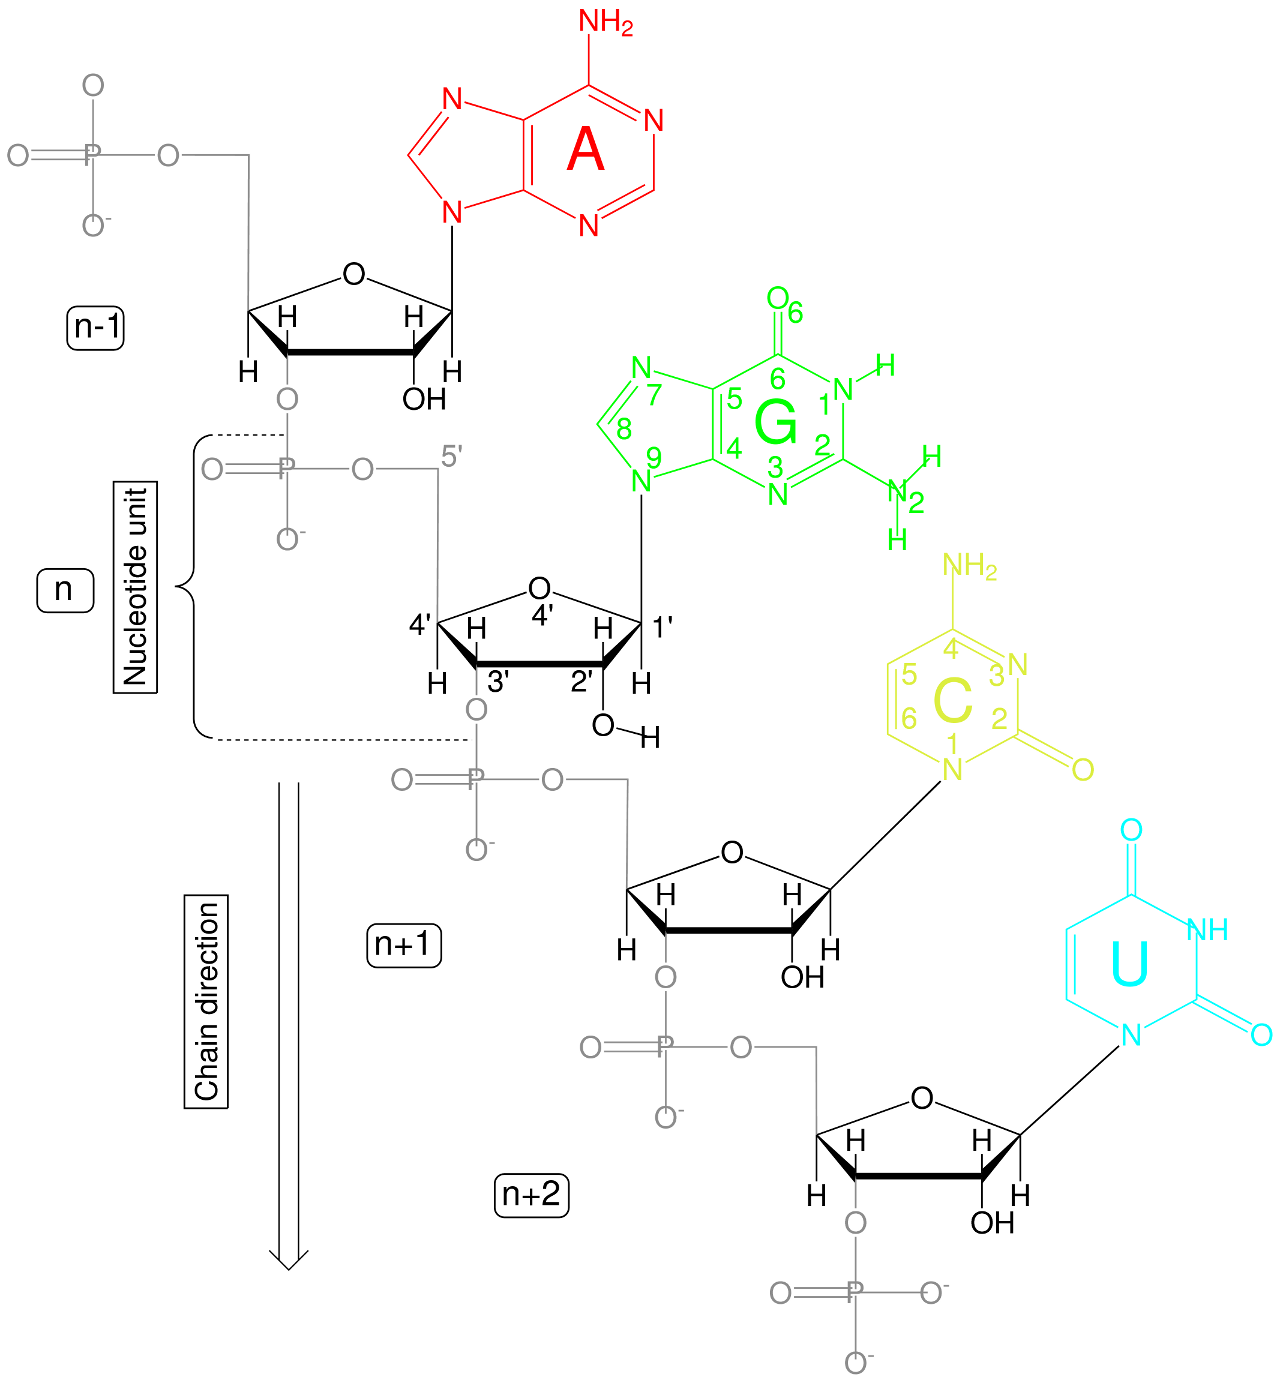
\includegraphics[scale=3.0]{Chapter1/chemistry1b.png}
\caption{A  single strand  of  RNA drawn  in  the 5$'$  to 3$'$  sense
  showing the  main chemical entities  which compose it;  base, sugar,
  and backbone.  The four bases (A,  G, C, U) are colored according to
  the  NDB  (Nucleic  Acid  Database)  convention  \cite{ndburl},  the
  backbone is colored gray, and the  sugars black. The bases G, and C,
  and the  furanose sugar  are numbered according  to the  IUPAC rules
  \cite{iupac1983}. This  figure is a  reproduction of Figure  2.1, in
  Wolfram Saenger's book \cite{saenger1984}.}
\label{fig:chemistry1}
\end{figure}  

Heterocyclic bases can form a diversity of base-pairs through hydrogen
bonding and  can be classified in  28 classes as  suggested by Saenger
\cite{saenger1984},   and  as   seen   in  Figure~\ref{fig:saenger28}.
Nomenclatures which  conform to Saenger's classes  have been developed
by Lee-Gutell \cite{lee2004}, Leontis-Westhof \cite{leontis2002b}, and
Lemieux-Major \cite{lemieux2002}.

\begin{figure}
\centering
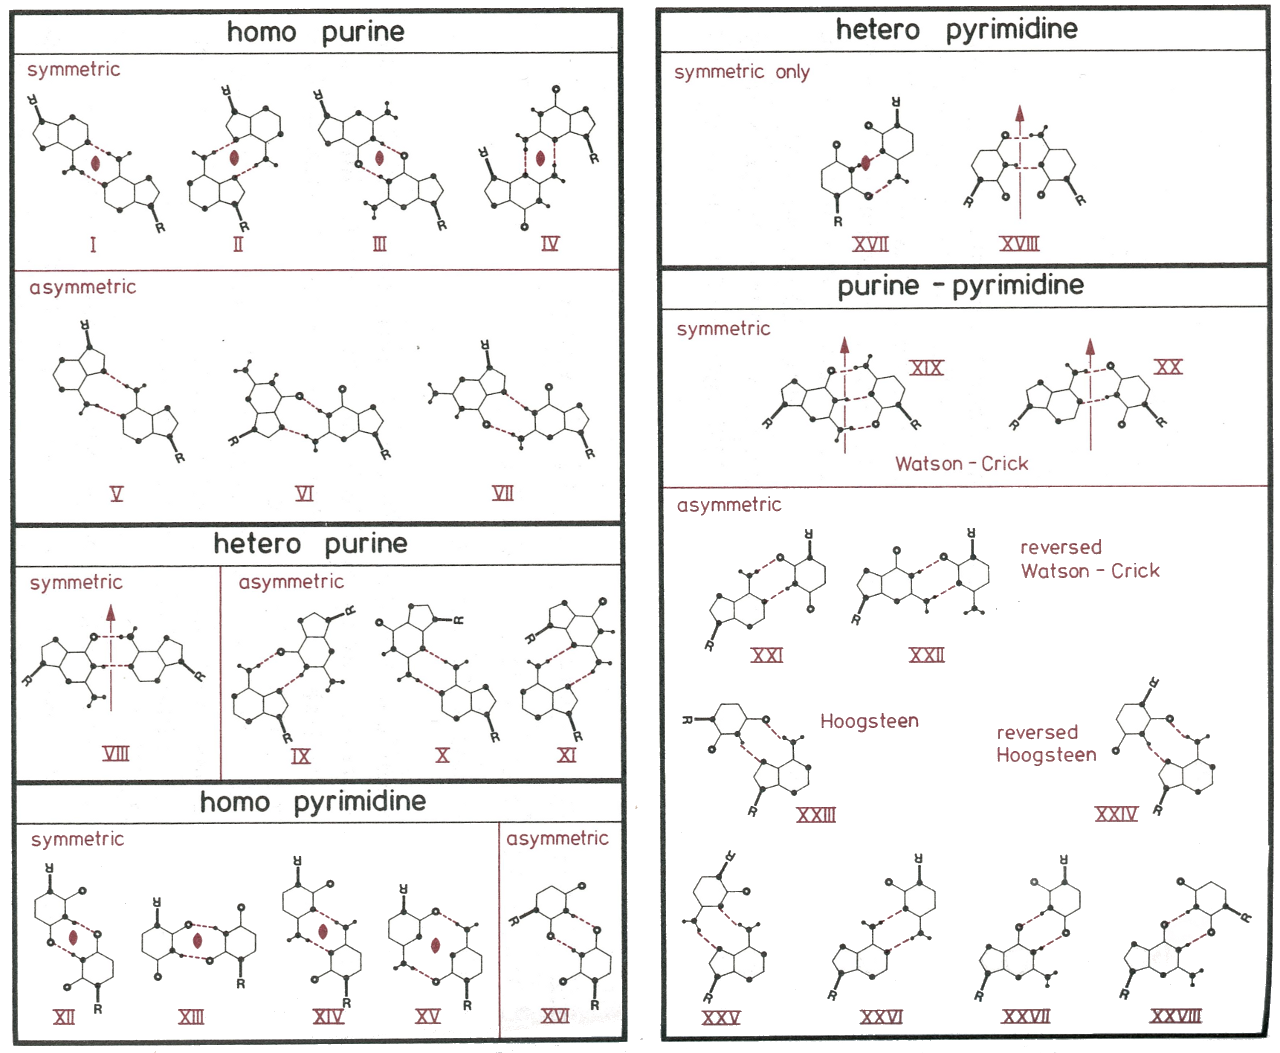
\includegraphics[scale=4.0, angle=90]{Chapter1/saenger28b.png}
\caption{Saenger  base-pairing  classes,  reproduced  from  his  book,
  "Principles of Nucleic Acid Structure". \cite{saenger1984}.}
\label{fig:saenger28}
\end{figure}  

The other non-covalent interactions which are common to the nucleotide
bases  are those  of  stacking through  London  dispersion forces  and
electrostatic  interactions.   It  has  been hypothesized  that  $\pi$
electron  interactions  could  also  account for  stacking,  but  very
precise quantum calculations \cite{sponer1996, sponer1997} have show
otherwise thus far.

Sugar, and  backbone can adopt a variety  of conformations constrained
to the values of their torsion  angles. In the case of the sugar these
torsion angles are called puckers,  perhaps in analogy to the gestures
made  by human  lips.   The prefered  sugar  pucker in  RNA is  called
C$_{3'-\textrm{endo}}$,  but in  cases where  an intercalated  base is
acommodated between two sequential  bases, the sugar pucker changes to
a non-prefered  conformation called C$_{2'-\textrm{endo}}$.  Standards
to  describe the  conformations resulting  from the  specific  sets of
torsion angle  values which sugars  and backbone can attain  have been
developed and can be seen  in textbooks \cite{saenger1984}, in the web
\cite{jenaurl}, and in  the IUPAC recommendations \cite{iupac1983}. We
refer the reader to these sources for a more detailed description, and
limit  ourselves  to  show  in Figure~\ref{fig:puckersbbone}  a  brief
description of these torsion angles.

\begin{figure}
\centering
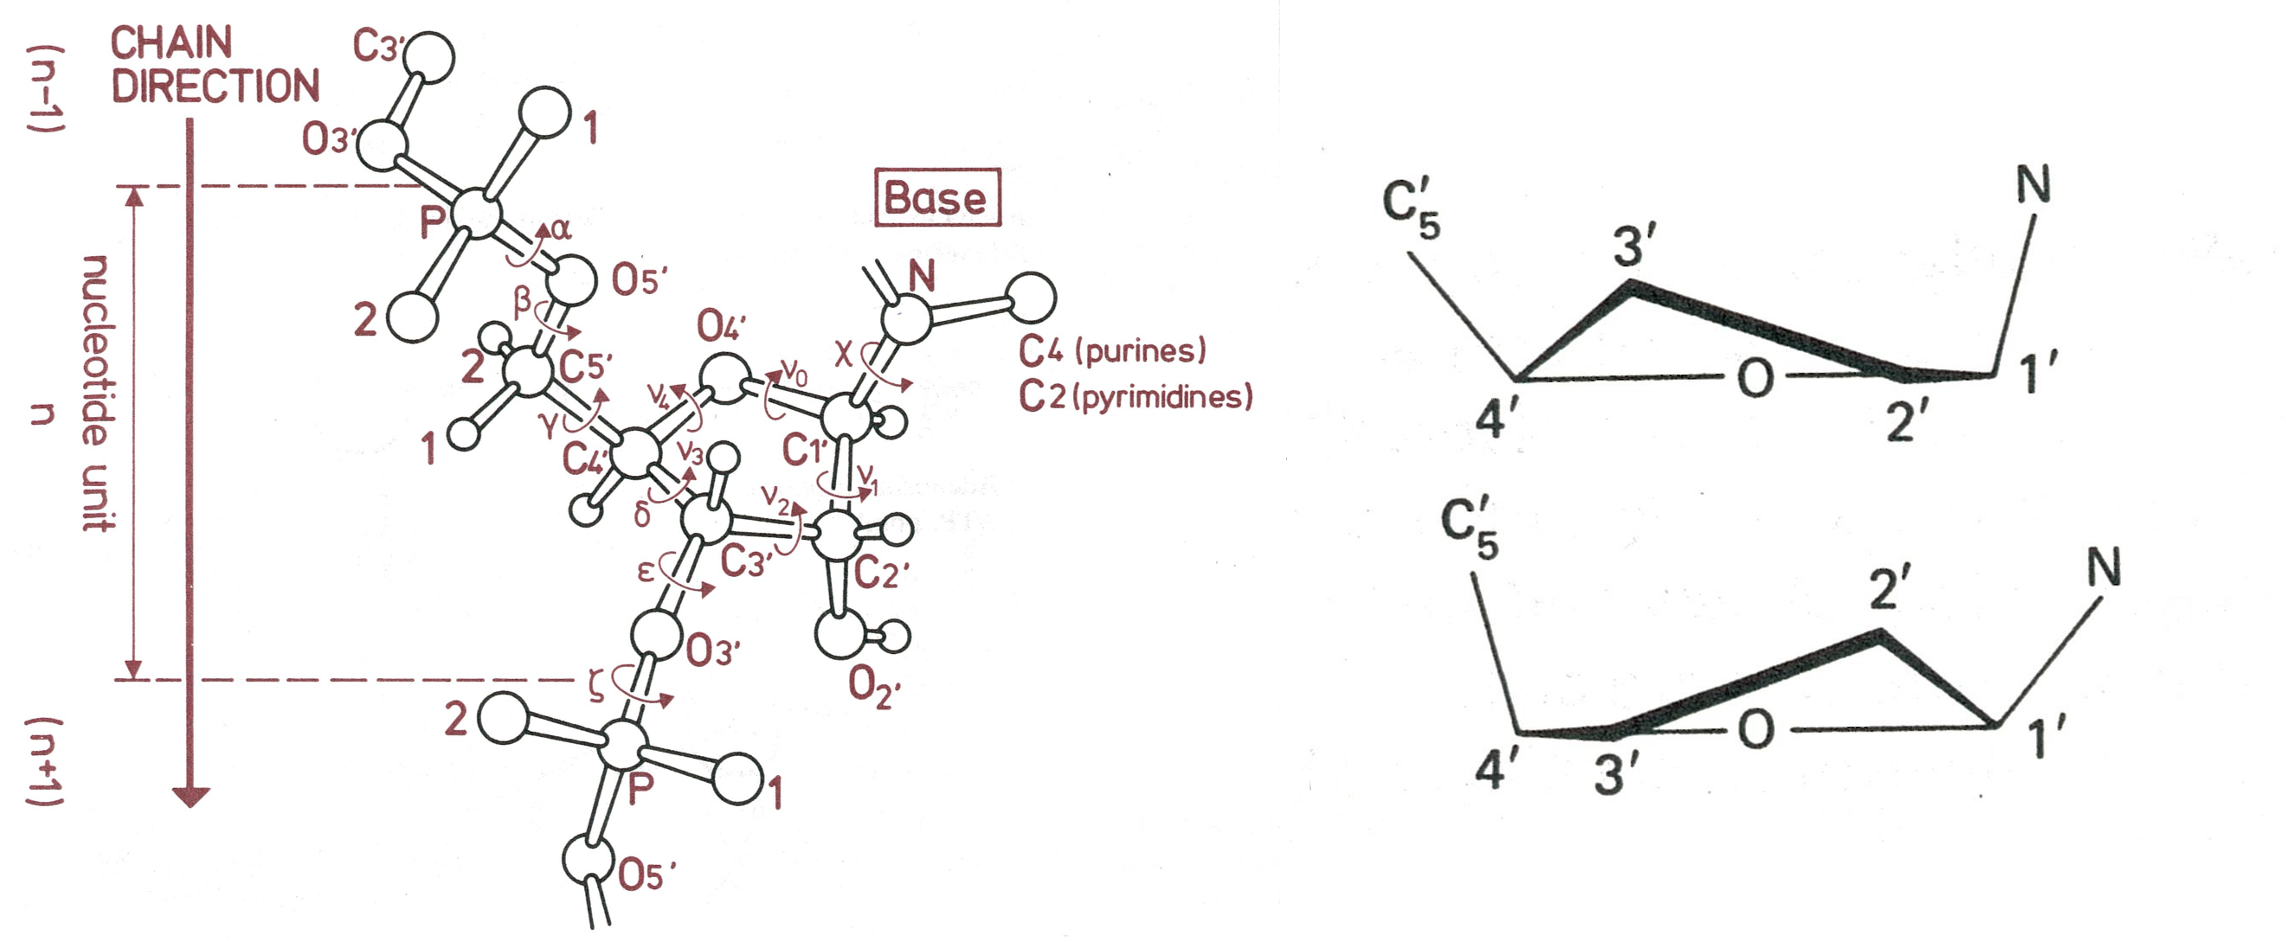
\includegraphics[scale=1.8, angle=0]{Chapter1/torsions.png}
\caption{\textbf{Left:}      Backbone      and      Sugar      torsion
  angles. \textbf{Right:}  The most common  sugar pucker conformations
  in  RNA,  that is,  C3'endo  and  C2'endo,  reproduced from  Wolfram
  Saenger's,         "Principles        of         Nucleic        Acid
  Structure". \cite{saenger1984}.}
\label{fig:puckersbbone}
\end{figure}  

%A-RNA 
%Loops
%Reference:
%Pure \& Appl. Chem., Vol.55, No.8, pp.1273—1280, 1983
%\url{http://www.fli-leibniz.de/ImgLibDoc/nana/IMAGE_NANA.html}


\section{RNA folding}
The first  high-resolution X-ray\index{X-ray} structure  of RNA larger
than a dinucleotide was  that of yeast tRNA$^{\textrm{Phe}}$ at 3{\AA}
in  1974 \cite{robertus1974,  kim1974, stout1976}.   Thirty  six years
later there  are two orders  of magnitude more  structural information
about RNA \cite{noller2005}, and new information from non-coding RNA's
is  expected  \cite{weinberg2009}.  This  fact  and  the discovery  of
ribozymes  \cite{kruger1982,  takada1983},  which  are  catalytic  RNA
molecules, has  renewed interest in solving  the RNA folding\index{RNA
  folding}  problem,  that is,  starting  from  the primary  sequence,
finding in  an automated\footnote{The term  automated is used  here to
  mean  a  theoretical model  of  tertiary  folding,  which could  use
  experimental measures of secondary structure association in the same
  way   that  the  traditional   secondary  structure   folding  model
  \cite{zuker1989,    hofacker1994}    uses    the    Tinoco-Uhlenbeck
  dinucleotide   postulate  \cite{borer1974}   to   find  total   free
  energies.}   way the  native three-dimensional  structure of  an RNA
molecule  and   the  folding  pathway   that  it  follows.    The  RNA
folding\index{RNA folding} problem is usually seen as analogous to the
protein folding  problem, due both  to the discovery of  the enzymatic
behavior  of  RNA \cite{kruger1982,  takada1983}  and the  complicated
folding of large RNA molecules \cite{batey1999}.  To take advantage of
this analogy,  a unified conceptual  framework for describing  RNA and
protein folding, called the  kinetic partitioning mechanism (KPM), has
been developed by Thirumalai and Hyeon \cite{thirumalai2005}. This and
other methods are based on defining an adequate partition function for
describing  the correct conformational  ensemble of  folded, partially
folded,    and   unfolded    structures    \cite{chen1995,   chen1998,
  thirumalai1996} of either protein or RNA.

\section{Is RNA folding a hard or easy problem?}
There  are  two trains  of  thought  regarding  the mechanism  of  RNA
folding.  One  states that  RNA folding is  less complex  than protein
folding  \cite{tinoco1999} because  RNA is  made up  of a  four letter
alphabet of similar  nucleotide units instead of a  20 letter alphabet
of  dissimilar   amino  acids.   Therefore  the   number  of  possible
sequential  combinations  is smaller.   It  is  also  well known  that
secondary and  tertiary interactions can  be separated in the  case of
RNA  by the absence  or presence  of Mg$^{2+}$  \cite{rangan2003} (see
Figure~\ref{fig:folding}), and  that the secondary structure motifs
of RNA are more limited  in  number  than  those  of protein,  whereas
secondary  and tertiary elements are not as easily separable in
proteins.
\begin{figure}[ht]
\centering
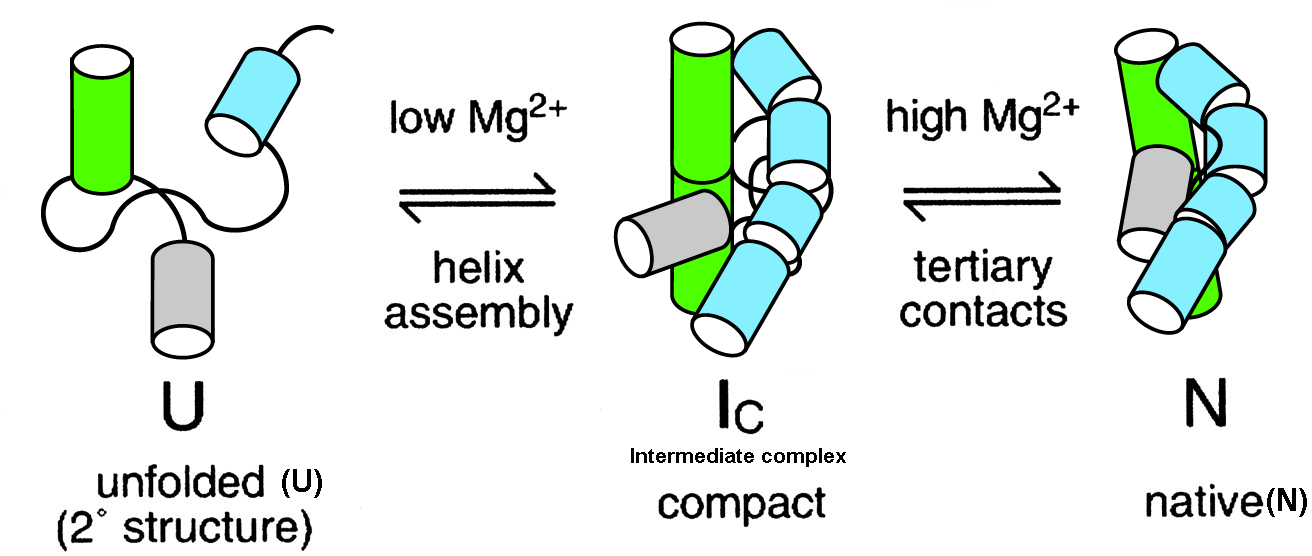
\includegraphics[scale=0.3]{Chapter1/rangan2003pnas.png}
\caption{Separation  of  secondary  and  tertiary interaction  in  RNA
  \cite{rangan2003}. Double helical secondary structure represented by
  individual  cylinders and  tertiary interactions  by  association of
  cylinders. Color coding stands for separate  helical regions of
  RNA, and the connecting  black strings represent single stranded loop
  structures.}
%% Note that Dr. Olson asks what the colors in cylinders mean.
%% Answer: They mean nothing. Perhaps only that the cyan stands for
%% the helical structures making a pseudo-knot, that is, P7 and P3.
\label{fig:folding}
\end{figure}
The  other point of  view says  that RNA  folding can  be at  least as
complex as protein folding \cite{moore1999a, sorin2004} since there is
no such thing  as hydrophobic burial of regions of RNA  as in the case
of  proteins.   Instead, the  electrostatic  problem  stemming from  a
complex charged backbone must be dealt with in the case of RNA.
% The case of the electrostatic treatment of the backbone is lacking
% here, most likely WKO wants me not to ignore our own Gerald Manning
% tinoco 1999 says this must be an easy to solve problem since we can
% do the electrostatics for it easily
For instance,  the interactions of  the RNA polyanionic  backbone with
water  and cations  \cite{klein2004a}  are not  easily simulated  with
explicit   solvent  models   like those used to treat   proteins.  The
aforementioned interactions of RNA  need to be modeled implicitly, and
must aim to describe long dynamic processes of the order of seconds to
minutes,  in  contrast   to  the  typical  time  scales   of  tens  of
microseconds associated with protein folding.
% Remember that this means that a explicit calculation for RNA would
% be prohibitively large.

Although   secondary   and  tertiary   structure   can  be   separated
experimentally, there have been few theoretical efforts to account for
the  folding  of  RNA  from  a random  sequence  of  nucleotides  into
secondary structures and tertiary  structures. What little is know has
been  investigated at  low resolution.  Stephen Harvey  and associates
have   simulated   the   folding   of   yeast   tRNA$^{\textrm{Phe}}$,
\cite{malhotra1990}  and  the  assembly  of  the 30S  subunit  of  the
ribosome \cite{stagg2003} at various levels of detail, initially using
only one pseudoatom  per helical region, and later  one pseudoatom per
nucleotide.  Recently  Fran\c{c}ois  Major's  group  at  Montreal  has
proposed a pipeline of two  computer algorithms to study RNA structure
\cite{parisien2008}.   One    pipeline   makes   secondary   structure
predictions, and the  other assembles 3D structures based  on the best
scoring secondary structures.
% Note for presentation ==> Include figure 1 in Malhotra-harvey paper
% Look at what says in folding.stanford.edu/science.html Also take
% into account Biophys J. V.88 2516-2524 for the case of having to
% think of water in the folding problem.
By contrast,  in the case of  proteins many groups  have simulated the
transition  from  secondary  to  tertiary  structure,  including  some
calculations which  account for the  strong coupling of  secondary and
tertiary  structure   \cite{westhead1999,  gerstein2003,  meiler2003}.
This type of work is  often referred to as protein structural topology
and there is no counterpart for RNA.

%The seminal paper here seems to be the one of liphardt in 2001 for
%rna unfolding
\section{Experimental folding techniques}
Traditionally   RNA   folding  and   unfolding   have  been   followed
calorimetrically  and spectroscopically as  a function  of temperature
and cation concentration  \cite{bloomfield2000, boots2008}. While this
approach  works well  for studying  two-state  folders, \textit{i.e.},
structures  which populate  only two  states (native  and  melted), in
general RNA's  are not  two-state folders. RNA  seems to go  through a
rugged  free  energy landscape  of  conformations  in  the process  of
folding \cite{zhuang2003}.  The  experimental solution to this problem
is offered  by single-molecule techniques  like fluorescence resonance
energy transfer (FRET) and  mechanical micromanipulation, in which the
ends of RNA  are attached to micron sized beads  which are then pulled
apart  and  monitored  with  a laser  light  trap  \cite{liphardt2001,
  onoa2004,  tinoco2004, hyeon2005}.  In  the case  of single-molecule
force-induced   unfolding,  state   transitions   often  occur   under
non-equilibrium  conditions, thereby  making it  difficult  to extract
equilibrium  information from the  data. Bustamante, Tinoco,
and associates have shown that by using the Crooks fluctuation theorem
\cite{crooks1999},  one  can deal  with  such  cases  and extract  RNA
folding    free     energies    from    single-molecule    experiments
\cite{collin2005}. Recently an alternative solution to this problem has
been proposed by Thirumalai and associates based on single-molecule
force-quenching experiments, by using a so called  de Genes "expanding
sausage model" \cite{hyeon2009}.
%\subsection{RNA Folding in Vitro vs in Vivo vs in Silico}
% It still is to be seen whether the following is relevant or not
% This single molecule information is
% collected in-vitro and not in-vivo, which is actually the ultimate
% problem aimed for prediction, there's quite a lot of evidence for
% different folding states reached in one case and not the other and
% viceversa \cite{sosnick2003, schroeder2002} but still a first step
% towards understanding in-vivo folding is in-vitro and in-silico
% experimentation.


\section{RNA simulations}
Network  and molecular  mechanics-molecular  dynamics (MM-MD)  methods
provide  useful  information  relevant  to the  RNA  folding-unfolding
problem, especially  for describing fluctuations away  from the native
conformation.   Gaussian network  models  \cite{y_wang2004, bahar1998,
  wang2005}, which  treat RNA  at less than  atomic detail,  have been
used  to  describe  the  motions  of large  RNA  structures  like  the
ribosome.  Examples  of the  predicted normal modes  of motion  of the
ribosome  can be  seen at:  http://ribosome.bb.iastate.edu/70SnK mode.
Using MM, Sanbonmatsu and coworkers  obtained a static atomic model of
the    70S    ribosome    structure    through    homology    modeling
\cite{tung2004}.  Tung  and  associates  used this  structure  for  an
all-atom  MD simulation  of the  movement of  tRNA into  a fluctuating
ribosome  \cite{sanbonmatsu2005}.  This  type of  simulation  might be
useful in a  reverse-folding approach to the RNA  folding problem.  To
the best of our knowledge,  such calculations haven't as yet been done
for RNA.

\subsection{Local nucleotide interactions}
%\subsubsection{QM approaches and MM consequences}
The molecular  interactions that  rule  RNA structures at  the nucleic
acid base level, \textit{i.e.},  local level, are hydrogen bonding and
stacking interactions. The former are  related to base pairing and the
latter, in most cases, to  nucleotide steps. These interactions can be
explored  theoretically at various  levels. At  the highest  level are
ab-initio  quantum   mechanical  calculations  which   are  still  too
expensive   for  systems  as   large  as   hundreds  of   atoms.  Such
calculations,  nevertheless,  can  tell   a  great  deal  about  local
electronic behavior.  For example, Hobza and  collaborators have found
that the  stacking interaction of free nucleotide  bases is determined
by   dispersion  attraction,   short-range  exchange   repulsion,  and
electrostatic  interaction.  No  specific $\pi-\pi$  interactions  are
found     from    electron    correlated     ab-initio    calculations
\cite{sponer1996, sponer1997}.  This is  why force field  methods have
been so successful in the  study of nucleic acids, since the empirical
potentials used  in such studies  mimic well the  quantum mechanically
obtained energy profiles \cite{tung2004, sponer2000}.
% since they can be modeled easily with simple empirical potentials
% consisting of Lennard-Jones, van der Waals and Coulomb terms.
% What the recent results say it's simply that by using a larger
% basis set, they can account for some interactions which were not
% included before, and maybe because of taking better account of
% electron-correlation.
A currently debated ab-initio finding is whether small fluctuations in
the   configurations   of   neighboring   base  pairs   (dimers)   are
iso-energetic  or  not.   Recent  calculations  of  Sponer  and  Hobza
\cite{sponer2006}    seem   to    contradict   their    earlier   work
\cite{sponer2000,  hobza2002},  in which  the  stacking energies  were
reported to  be relatively insensitive to dimer  conformation. The new
results  use  the so-called  ``coupled  cluster  singles doubles  with
triple electron excitations'' CCSD(T)  method, to account for electron
correlation.  Using  this electron correlation  energy correction, the
stacking energy differences between dimer conformations turn out to be
considerably higher than previously reported.

% therefore justifying rigid body parameter interpretations.
% \subsubsection{Experimental Stacking and Polyionic backbone}
Single-strand and double-strand stacking free energies can be obtained
calorimetrically \cite{freier1985}.   One of the  most popular methods
used   for  obtaining   such  quantities   is   differential  scanning
calorimetry (DSC) \cite{marky1982}.  These measurements show favorable
dinucleotide stacking  free energies as  large as $-3.6$  kcal/mol for
double-strand  stacking.   Experimentally,  the  magnitudes  of  these
interactions      are     found      to      be     sequence-dependent
\cite{bloomfield2000}. In  fact, the  stacking free energies  for some
sequences\footnote{Free   Energies   for   5'   unpaired   nucleotides
  (e.g. UC/A  UU/A) are quite small  (i.e.  $<$ 0.4  kcal/mol) and are
  termed  weakly stacking bases.\cite{burkard1999,  burkard1999b}} are
found to  be negligible.   Thus there may  be no  accountable stacking
interaction at all for some sequences.

Besides  taking into  account  the effects  of  stacking and  hydrogen
bonding,  it  is  important  to  think  at the  same  time  about  the
polyelectrolyte  nature  of the  RNA  backbone.  Manning's  counterion
condensation theory \cite{manning1977,  manning2003} provides a simple
and   quantitative  picture   of   the  interactions   of  a   regular
double-helical  nucleic acid  polyanion with  its counterions,  but it
does   not  take   into  account   the  discrete   nature   of  charge
\cite{bloomfield2000} or the  folding of RNA. Poisson-Boltzmann theory
offers a more detailed picture of the behavior of charged macroions in
solution \cite{antypov2005, xu2007}.
% Talk more about counterion condensation, thirumalai discusses it on
% his 2001 paper also chapter 8 of Bloomfield, Crothers, Tinoco
% (References \cite{manning2003} Ray-Manning?).
% Real Experiments results for stacking energies and polyanion
% energies and Energetics related to cation metal presence
% WKO says that there might be old experimental data that are contrary
% to this and that I must show it here, so far what I've found is
% Saenger saying that based on old QC and this is different, he
% relates it to hydrophobicity concepts. Talk about experiments.

The local conformational  space of RNA has been  studied using a large
set of available  RNA structures from the Nucleic  Acid Database (NDB)
\cite{berman1992}.  The  torsion angles  of the nucleotide  steps have
been   clustered    using   different   techniques   \cite{murray2003,
  schneider2004}.   The  root-mean-square  deviations  (RMSD)  of  the
distances between closely spaced  atoms in the phosphates, sugars, and
bases, have  also been clustered \cite{sykes2005}.  The latter studies
are aimed  at finding the  common nucleotide base steps  and base-pair
building  blocks which  have  been  given the  name  of RNA  doublets.
Recently, the  RNA Ontology Consortium (ROC) has  proposed a consensus
set  of RNA dinucleotide  conformers integrating  the work  of various
groups \cite{richardson2008}.


\subsection{RNA  secondary  structure   algorithms  and  the  lack  of
 tertiary ones}
From   secondary   structure   prediction  algorithms   like   Zuker's
\textit{mfold} program \cite{zuker2003}, Hofacker's Vienna RNA package
\cite{hofacker1994}, or  Mathews Dynaling software \cite{mathews2002},
one obtains  a large ensemble  of secondary structure graphs,  i.e. 2D
representations of  the double-stranded helical  stems, hairpin loops,
bubbles formed by the constituent bases.  These graphs can be analyzed
with graph  theory to produce  a partition function describing  a full
arrangement  of contacts for  the total  number of  possible secondary
structures, allowing  the construction  of a "relation  of microscopic
conformations to macroscopic  properties" \cite{chen2000}. So far this
type of model  has not been generalized to  take into account tertiary
structural features, \textit{i.e.},  interhelical interactions of RNA.
In  the  last  two to  three  years  a  boom  in prediction  of  small
($\approx$ 200  nucleotides) RNA 3D structures  has started. Basically
three types of approaches are being  followed.  One is that of using a
coarse-grained model, assigning a potential function to it, applying a
minimization procedure, and then performing a molecular mechanics (MM)
all-atom  refinement \cite{das2007,  ding2008,  jonikas2009a}. Another
starts  from  the predicted  secondary  structures,  assumes that  the
helical  regions adopt  the canonical  A-form  structure, mechanically
inserts residues as rigid bodies in the remaining non-helical regions,
and  finally carry  out an  MM optimization  \cite{martinez2008}.  The
third  approach   entails  a  pipeline   between  secondary  structure
prediction, and tertiary structure assembly is proposed. This pipeline
uses  as bridging  concept  between  2D and  3D  structure, the  graph
theoretical definition of a minimum cycle basis, which for the case of
nucleic  acids  has  been  renamed  as  Nucleic  Cyclic  Motifs  (NCM)
\cite{parisien2008}.

\subsection{RNA  overall fold}
Whereas  in  the case  of  proteins  one  qualitatively describes  the
overall  fold  in terms  of  the  arrangement  of secondary  structure
motifs, \textit{i.e.}, using the helix-ribbon-coil images developed by
Jane           Richardson          \cite{richardson2000}          (see
Figure~\ref{fig:ribboncoil}), there is still no comparable description
of  the overall  fold of  RNA. A  ribbon representation  of  the sugar
phosphate backbone (see Figure~\ref{fig:ribosome}) helps to understand
the  folding of  small  RNA's, but  in  the case  of  the ribosome,  a
representation at such level of detail does not allow to make sense of
such  a large  structure  (close  to 3000  nucleotides  for the  large
subunit of  the archaeal  ribosome).  In the  past two  years Holbrook
\cite{holbrook2008}  and  Sykes  \cite{sykes2009}  have  proposed  new
representations for RNA based on helical region organization. Holbrook
makes  an  analysis of  continuous  interhelical  strands, so  called,
COINS, and Sykes makes an optmized projection of 3D helical axis to 2D
images,  which can  later  be annotated  with,  for example,  hydroxil
radical footprinting results.

\begin{figure}[ht]
\centering
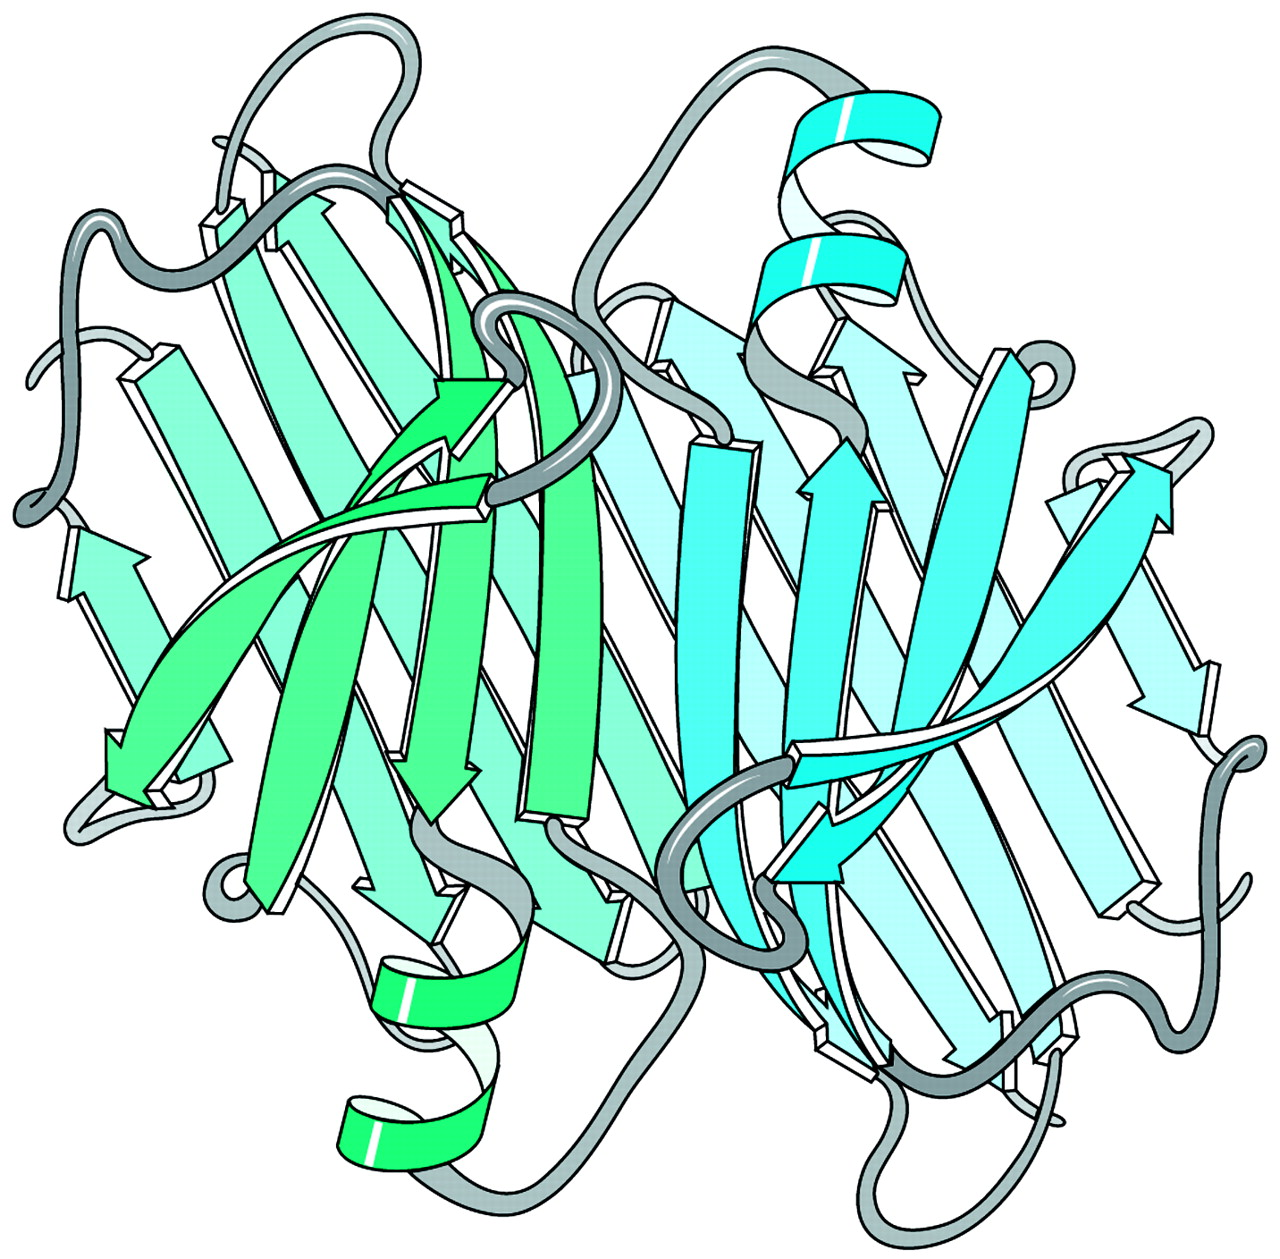
\includegraphics[scale=0.4]{Chapter1/overallfold.png}
\caption{Ribbon-coil    schematic    illustraring    the   fold    and
  intermolecular  units of  a dimer  of prealbumin  (PDB\_ID:2pab), or
  transthyretin,    taken     from    Richardson    \textit{et    al.}
  \cite{richardson2002}}
\label{fig:ribboncoil}
\end{figure}

\begin{figure}[t]
\centering
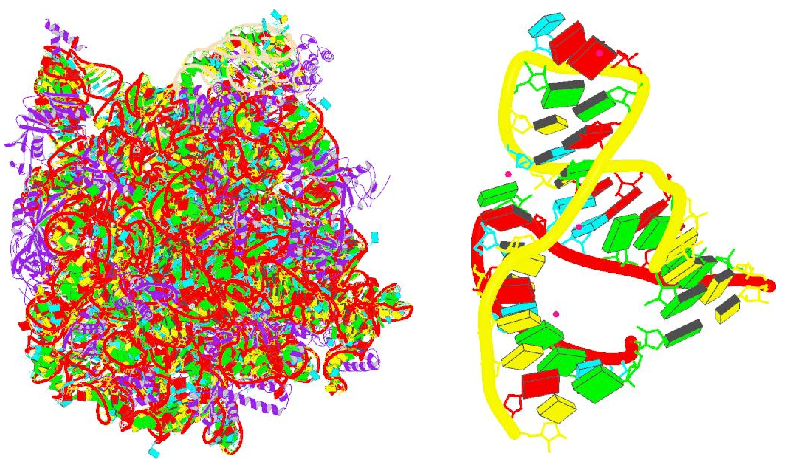
\includegraphics[scale=0.5]{Chapter1/ribosome_ribozyme.png}
\caption{Images   of  the  \textit{Haloharcula   marismortui's}  large
  ribosomal subunit NDB\_ID:RR0033 (left) and the hammerhead ribozyme
  (right) NDB\_ID:UR0029.
  The  figures were taken directly  from the NDB
  web  pages,   and  show  a  3DNA   generated  \cite{lu2008b}  ribbon
  representation of the phosphate backbone, and a block representation
  for the nucleotide bases. From  the figures it's clear that, whereas
  the   ribozyme   fold   can   be  clearly   understood   with   this
  representation, the ribosome fold cannot.}
\label{fig:ribosome}
\end{figure}

One  can  envision that  a  thorough  investigation  of the  space  of
translational and rotational degrees of freedom of the helical regions
of RNA could give clues as to  how we might see an overall fold in RNA
structures.  To the  best  of  our knowledge  there  is no  comparable
quantitative description of the folding of proteins.

In  the  case  of  proteins  the SCOP  (Structural  Classification  of
Proteins)  database  \cite{andreeva2004},  classifies proteins,  among
various  qualitative  descriptors,   according  to  folds,  which  are
recurrent  arrangements of  secondary structure,  that is,  a  list of
secondary  structures with  unique topological  connections.  The SCOR
(Structural  Classification  of  RNA)  database  \cite{klosterman2002,
  klosterman2004}, aims  to provide  a similar classification  to that
obtained   for  proteins,   but   using  RNA   motifs  instead.   This
classification focuses on the local folding of small pieces of RNA and
cannot  describe  the  overall  fold.  Local  classification  is  also
qualitative rather than quantitative.

\subsection{RNA motifs}
The term ``\textit{RNA motif}'' is  used in the literature to describe
three   different   levels    of   RNA   organization,   namely,   RNA
\textbf{sequence} motifs, RNA  \textbf{secondary structure} motifs, or
RNA \textbf{3D structure} motifs.   Because these distinctions are not
always clearly made the beginner may result in confused and frustrated
bibliographical searches.

The lack of a unique definition of RNA motifs is yet another source of
confusion  in  understading  RNA  motifs  is  the  lack  of  a  unique
definition.  Three  popular and  somewhat  recent  definitions of  RNA
motifs include:
\begin{itemize}
\item{``\textit{a discrete sequence or combination of
    base  juxtapositions   found  in  naturally   occurring  RNA's  in
    unexpectedly high abundance.}''\cite{moore1999}}
\item{``\textit{conserved structural subunits that make
    up the secondary structures of RNAs.}''\cite{holbrook2005}}
\item{``\textit{ordered   stacked    arrays   of
    non-Watson-Crick  base  pairs  that  form distinct  folds  on  the
    phosphodiester backbones of RNA strands.}''\cite{leontis2003}}
\end{itemize}

The  kind of RNA  motifs addressed in this
thesis are of the third type, that is, RNA \textbf{3D structure}
motifs  which we henceforth term RNA  motifs.
From our point of view RNA motifs are to be understood as  peculiar
sets of geometrical  (in the rigid block sense)  arrangements in
three-dimensional space.

Even  though there  is no  unique definition,  we can  think  of three
practical  tasks regarding  RNA  motifs.   That is,  given  an RNA  3D
structure automatically identify, describe,  and find new motifs.  For
automatic  identification of  RNA motifs  Pyle and  collaborators have
developed  a software called  AMIGOS. This  software finds  RNA motifs
based on  specific values of backbone virtual  torsion angles $\eta$
and  $\theta$  \cite{olson1980, malathi1985,  duarte2003} in  a  way  which
resembles   a   Ramachandran  plot   analysis.    Lemieux  and   Major
\cite{lemieux2006}  provide  the  software MC-Fold,  which  implicitly
finds RNA motifs based on  an algorithm to determine so called nucleic
cyclic  motifs, which  are  just the  minimal  cycle basis  of an  RNA
secondary  structure  interpreted as  a  mathematical graph.   Leontis
\cite{nasalean2009}  and collaborators  provide FR3D  (read  as FRED).
F3RD is  a matlab  windows executable program  which finds  RNA motifs
based on the isostericity matrices of base-pairs.

For description of RNA motifs Schlick and collaborators have used FR3D
to  localize  RNA helical  junctions  of  order  four (i.e.   four-way
junctions) or  higher, and performed a  visual analysis to  see if the
helices  in  such junctions  form  coaxial  stacks  or not,  and  have
classified   them   accordingly   \cite{laing2009,  laing2009a}.    As
mentioned previously in the context of RNA folds, Holbrook, and Sykes,
describe   helical  regions  and   display  them   in  two-dimensional
representations. Sponer's group has carried out the description of RNA
motifs present  in the ribosome using Molecular  Dynamics (MD) methods
implemented  in   the  AMBER   package.   They  have   performed  25ns
simulations  of   the  Sarcin-Ricin  Domain  (SRD)   of  the  ribosome
\cite{spackova2006}, and also 80ns  simulations of hydration of loop E
in the 5S subunit of the ribosome \cite{reblova2003}.

The software programs which perform the task of identifying RNA motifs
in RNA structures also have the ability to find new RNA motifs, as is
the case for AMIGOS, MC-Fold, and FR3D.

\section{Overview}
Keeping always in  mind the greater scope of  the RNA folding problem,
this thesis  addresses various issues of  RNA structural understanding
using RNA crystallographic data from the Protein Data Bank (PDB). Such
data  has been  analyzed statistically  in terms  of a rigourous
rigid-body formalism.  In Chapter 2 the consensus clustering technique
is   used  to   classify   RNA  base-step   parameters  of   non-A-RNA
conformations, and  the resulting groups are  localized and understood
in the context  of rRNA.  Chapter 3 reconsiders  previous work carried
out by  Dr. Yurong Xin  at the Olson's  lab, on classification  of RNA
base-pairs by  resorting again to clustering  analysis techniques, and
database  mining  of the  WWW  available  Base  Pair Structures  (BPS)
database.  In  Chapter 4 we  explore, using statistical  analysis, the
data available  on RNA  helical regions, and  use this  information to
compute the persistence length of double-stranded RNA's and compare it
to  experimental  results.  In  Chapter  5 we  provide  a  new  python
software,  pyRNAmotifs which interfaces  with 3DNA  to do  a rigourous
search of existing and perhaps  new RNA motifs, and finally in Chapter
6  we propose  the measurement  and classification  of  RNA structures
using a  new graph theoretical index  named folding index,  based on a
helical region "view"  of RNA's, which is clearly  concordant with the
emerging  necessity   of  new  metrics  beyond   RMSD  for  structural
understanding.

\bibliography{biblio}

%2345678901234567890123456789012345678901234567890123456789012345678901234567890
%%%%%%%%%%%%%%%%%%%%%%%%%%%%%%%%%%%%%%%%%%%%%%%%%%%%%%%%%%%%%%%%%%%%%%%%%%%%%%%%
% MAURICIO ESGUERRA NEIRA
% Ph. D. Thesis
%%%%%%%%%%%%%%%%%%%%%%%%%%%%%%%%%%%%%%%%%%%%%%%%%%%%%%%%%%%%%%%%%%%%%%%%%%%%%%%%
\chapter{RNA Base Steps}
\label{basesteps} 
\bibliographystyle{nar}
The problem of classification of the space of conformations
%configurations?
of RNA  is not  new, see for  example, Olson  1972 \cite{olson1_1972},
Saenger     1984     \cite{saenger1984},     and    Gautheret     1993
\cite{gautheret1993}.  Although only  a few researchers addressed this
problem  before  the  turn  of  the twenty  first  century,  now  this
situation is changing rapidly. The reason for this fast change came in
the year 2000, when a vast amount of RNA structural information became
available  upon the  elucidation of  the  structure of  the 30S  small
ribosomal  subunit  of   \textit{Thermus  thermophilus},  a  bacterial
ribosome  \cite{wimberly2000,  schluenzen2000},   and  the  50S  large
ribosomal subunit of \textit{Haloarcula marismortui}, an archaeal
%\footnote{I emphasize the  phylogeny of rRNA's here since  there is an
%  ongoing discussion among biologists on whether archaea are closer to
%  prokaryotes, or to eukaryotes.}
ribosome \cite{ban2000}.
\begin{figure}[H]
\centering
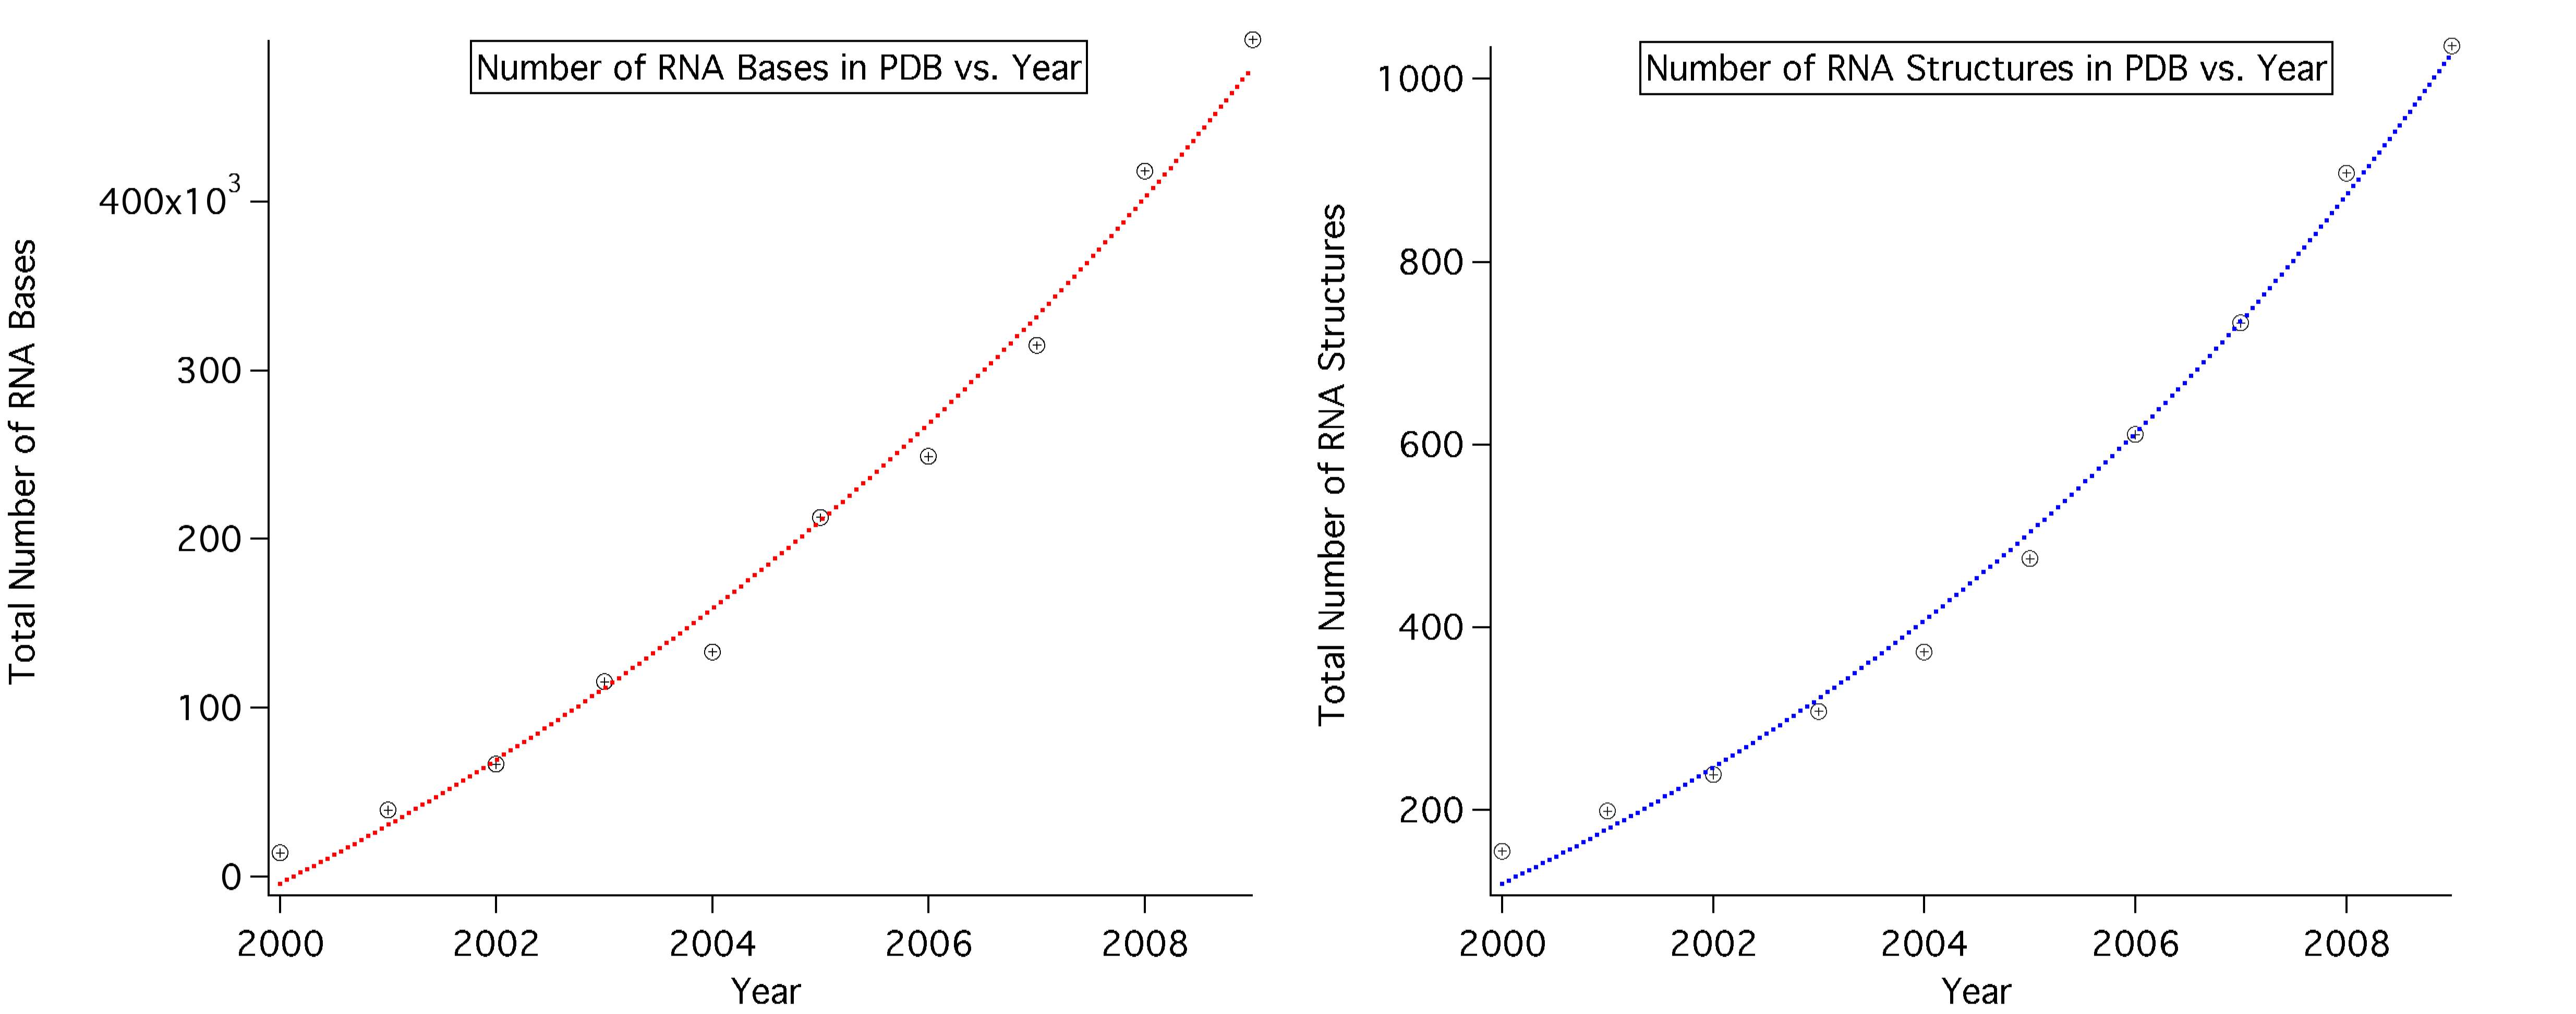
\includegraphics[scale=0.38]{Chapter2/rna2000_2009copy.png}
\caption{\textbf{Left:} Total number of RNA bases added to the Protein
Data Bank (PDB)  database between 2000 and 2010  (exponential fit line
in blue). \textbf{Right:} Total number of RNA structures solved yearly
by X-ray  crystallography between 2000 and 2010  (exponential fit line
in red).}
\label{fig:rnainpdb}
\end{figure}

\noindent Between  1978 and  2000 a total  of 116 RNA  structures with
resolution better than 3.5  \AA, and comprising around 5500 nucleotide
bases were added to the Protein  Data Bank (PDB), and between 2000 and
today  931  RNA\index{RNA}  structures  comprising  491158  nucleotide
bases.  That  is, the increase in  information due to  the solution of
large  RNA structures as  pointed out  by Noller  \cite{noller2005} is
about two  orders of  magnitude. It  is clear from  the growth  of RNA
structural  information from  2000  until today  that  both the  total
number of RNA structures deposited in the PDB, and the total number of
nucleotide bases in these  structures, is increasing at an exponential
rate  (as can  be seen  from  the exponential  fits of  these data  in
Figure~\ref{fig:rnainpdb}).  It is important  to note that such growth
comes mainly from ribosomal structures which contain 88 percent of all
RNA bases in  the PDB.  So, even though structural  interest in RNA is
growing  since  ribosomal structures  became  available  in 2000,  and
several Nobel prizes  have been awarded for work  in this field, along
with   the   exciting   possibilities   of   deciphering   large   RNA
\cite{weinberg2009}  structures  other than  the  ribosome, still  the
growth of  the RNA structural  field is far  from that of  proteins if
weighed by  the growth in  diversity of RNA structural  information in
the past decade.  If we look  at the current distribution of the sizes
of  RNA   structures  counted  in   terms  of  the  number   of  bases
(Figure~\ref{fig:rnaranges}) it is clear  that there are large patches
where there are  no RNA structures whatsoever.  That  is, there are no
solved structures  of RNA with  roughly 600 to  1400 bases or  1800 to
2700  bases.  The  area of  non-coding RNA's  holds great  promise for
finding structured RNA's  in such length ranges, as  has recently been
suggested by Breaker \cite{weinberg2009}.  A representative example of
the characteristic ranges  of RNA structures available to  date in the
PDB can be seen in Table~\ref{tab:rnarange} for structures larger than
300  bases. A  comparison between  the total  number of  structures of
protein, protein plus nucleic acid, DNA, and RNA, available at the PDB
from   the  seventies   until  today   can  be   seen   in  Supplement
Figure~\ref{fig:allpolypdb}.  The most  notable feature of this figure
is  the  large difference  between  the  number  of deposited  protein
structures and  nucleic acid structures, which have  to be represented
with an offset  of an order of magnitude in  number of structures. The
other prominent feature is that of the difference in growth of DNA vs.
RNA structural information. RNA structures seem to be growing steadily
since the mid-nineties, whereas DNA structural information seems to be
tending to a constant number, or having a very small growth.
\begin{figure}
\centering
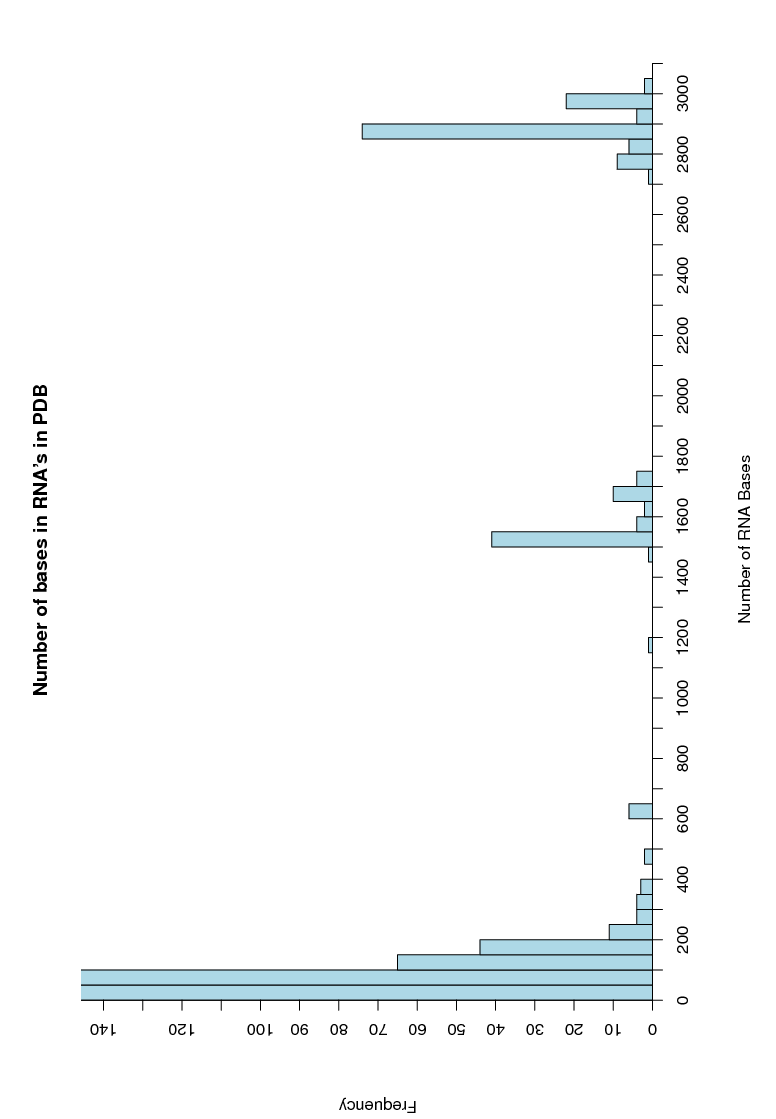
\includegraphics[scale=0.60, angle=270]{Chapter2/histogram.png}
\caption{Frequency of  nucleotide bases in RNA molecules  found in the
  PDB classified by  the size of RNA molecules. We  define the size as
  the total number of nucleotide bases present per molecule.}
  \label{fig:rnaranges}
\end{figure}
%The table and Figure 1.1 come from downloading all structures from
%2000, until today that have RNA in the pdb and that have a resolution
%better that 3.0A, they are 460 structures.

\noindent The analysis of  the conformational information contained in
RNA  structures  can  be  divided  into three  main  perspectives:  an
atom-based perspective; a bond-based  perspective; and a third, as yet
unexplored  to our  knowledge, rigid-body-based  perspective.   In the
atom-based perspective,  either a  direct comparison of  backbone atom
positions  is  made  \cite{reijmers2001},   or  a  comparison  of  the
distances between  a reduced  set of atoms  taken from  the nucleotide
backbone, sugar,  and base  \cite{sykes2005} is made.   The bond-based
perspective  is  divided  into   three  main  categories.   The  first
considers the consecutive  covalent bonds in the RNA  backbone and the
glycosidic  bond between  the sugar  and base,  that is,  six backbone
torsion  angles and one  glycosidic torsion  angle \cite{reijmers2001,
murray2003,  hershkovitz2003,  schneider2004,  hershkovitz2006}.   The
second   considers  the   pseudo-bonds  between   consecutive   P  and
C4$^{\rm{\prime}}$  atoms  and  the  resulting  pseudo-torsion  angles
$\eta$   and  $\theta$   \cite{olson1_1972,   duarte1998,  duarte2003,
wadley2007} \footnote{Previously  the pseudotorsion angles  $\eta$ and
$\theta$     were    given     the    names     $\omega_{\nu}$,    and
$\omega_{\nu'}$.\cite{olson1980,  malathi1985}}.   The third  category
considers the networks of  horizontal hydrogen bonding patterns coming
from  a definition of  interacting edge  boundaries in  the nucleotide
bases \cite{westhof2000, leontis2002, leontis2006}. In this chapter we
study the  rigid-body based perspective using  clustering analysis and
discuss  the  relationship  of  these  findings  to  other  previously
reported perspectives on RNA conformation.
\begin{table}[htbp]
\begin{center}
{\small
\begin{tabular}{c|p{5cm}|c|c|c}
\hline
\bf{PDBID} & \bf{Structure Name} & \bf{Phylogenetic Group} & \bf{Number of bases} & \bf{Year} \\ \hline
1l8v & Mutant of P4-P6 Domain of Group I Intron & Eukaryote & 314 & 2002 \\ \hline
3igi & Group II Intron & Bacteria & 395 & 2009 \\ \hline
1fg0 & Central Loop in Domain V of 23S rRNA & Archaea & 499 & 2000 \\ \hline
2nz4 & GlmS Ribozyme & Eukaryote & 604 & 2006 \\ \hline
1xmq & 30S rRNA & Bacteria & 1522 & 2004 \\ \hline
1ffk & 50S rRNA Subunit & Archaea & 2828 & 2000 \\ \hline
\end{tabular}
}
\caption{Some large  RNA structures  ($>$300 bases) elucidated  in the
  last decade.}
\end{center}
\label{tab:rnarange}
\end{table}

\section{Consensus Clustering of Single Stranded Base Step Parameters}
To  our  knowledge there  has  been  no  classification of  rigid-body
base-step parameters for the RNA  structures now available in the PDB.
It is important to note here that in crystal structures, the RNA bases
are determined  more accurately than  the backbone torsion  angles, as
has been  shown by Richardson  and collaborators from the  analysis of
van  der Waals  steric  clashes.  This  can  be seen  more clearly  in
Figure~\ref{fig:murray},    reproduced    from    Richardson's    work
\cite{murray2003}, where the red and orange dots in the backbone atoms
region denote steric clashes and the green and yellow dots in the base
atoms region  denote very good  agreement with expected van  der Waals
distances.
\begin{figure}[htbp]
 \centering
 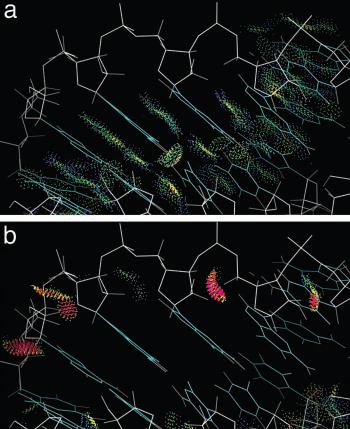
\includegraphics[scale=0.5]{Chapter2/murray2003.png}
 \caption{Comparison of base vs.  backbone structure in RNA reproduced
with permission from Jane  Richardson \cite{murray2003}. Here the blue
and green  dots in (a) denote  very accurate van  der Waals distances,
and the  red and orange  dots on (b)  denote steric clashes,  that is,
distances outside the acceptable van der Waals range.}
 \label{fig:murray}
\end{figure}

\subsection{Combining Fourier Averaging Results and Clustering Analysis}
We   used   standard   clustering   analysis  (CA)   techniques   (see
Appendix~\ref{appendix_a}) to classify  the non-ARNA base-steps in the
coordinate files of 20 rRNA  structures grouped in torsion angle space
by  Schneider  at  al.\cite{schneider2004}.  Here  we  describe  these
structures in terms of the  base-step parameters space. That is, three
translational parameters  (Shift $D_x$, Slide $D_y$,  Rise $D_z$), and
three   rotational  parameters  (Tilt   $\tau$,  Roll   $\rho$,  Twist
$\omega$), in the hexaparametric vector $\nu$:
\begin{gather}
\nu = (D_x, D_y, D_z, \tau, \rho, \omega)
\end{gather}
The    results    illustrated    in    the   dendrogram    shown    in
Figure~\ref{fig:eucl_cons}  were  obtained  by  performing  clustering
analysis  and  consensus  clustering  on  20  structures  provided  by
Schneider et al.   \cite{schneider2004}. These twenty structures which
are  illustrated  in Figures~\ref{fig:nonAclus}  and~\ref{fig:steps2},
were  obtained by  Schneider et  al. by  applying a  Fourier averaging
technique and  lexicographical clustering to the  torsion angles found
in the large subunit of ribosomal RNA (PDB\_ID:1jj2).  The methodology
we used follows  the approach taken by others  to recover the Periodic
Table  classification of the  elements from  multidimensional property
vectors of the elements \cite{restrepo2004, restrepo2006}.
\begin{figure}[htbp]
 \centering
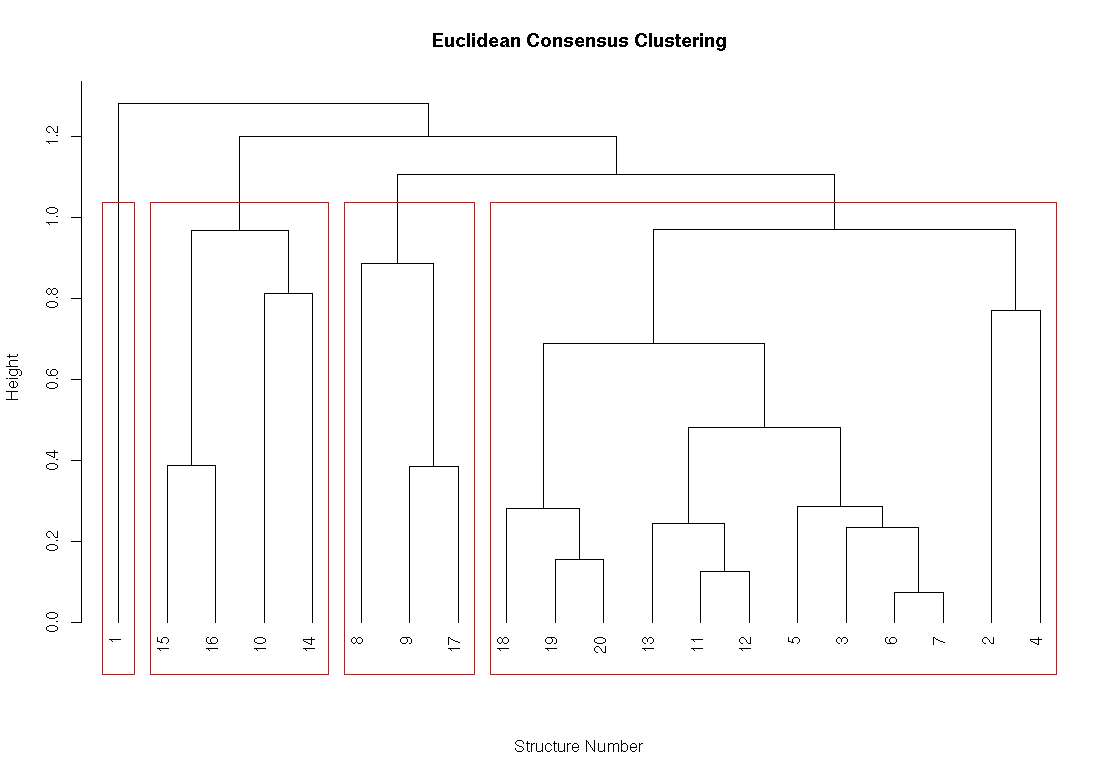
\includegraphics[angle=90, scale=0.6]{Chapter2/eucli_cons_nonA-RNA.png}
\caption{Dendrogram showing the results  of consensus clustering of 20
non-A-type  rRNA  dinucleotides   according  to  their  hexadimensional
base-step parameter vectors.}
 \label{fig:eucl_cons}
\end{figure}

\begin{figure}[htbp]
 \centering
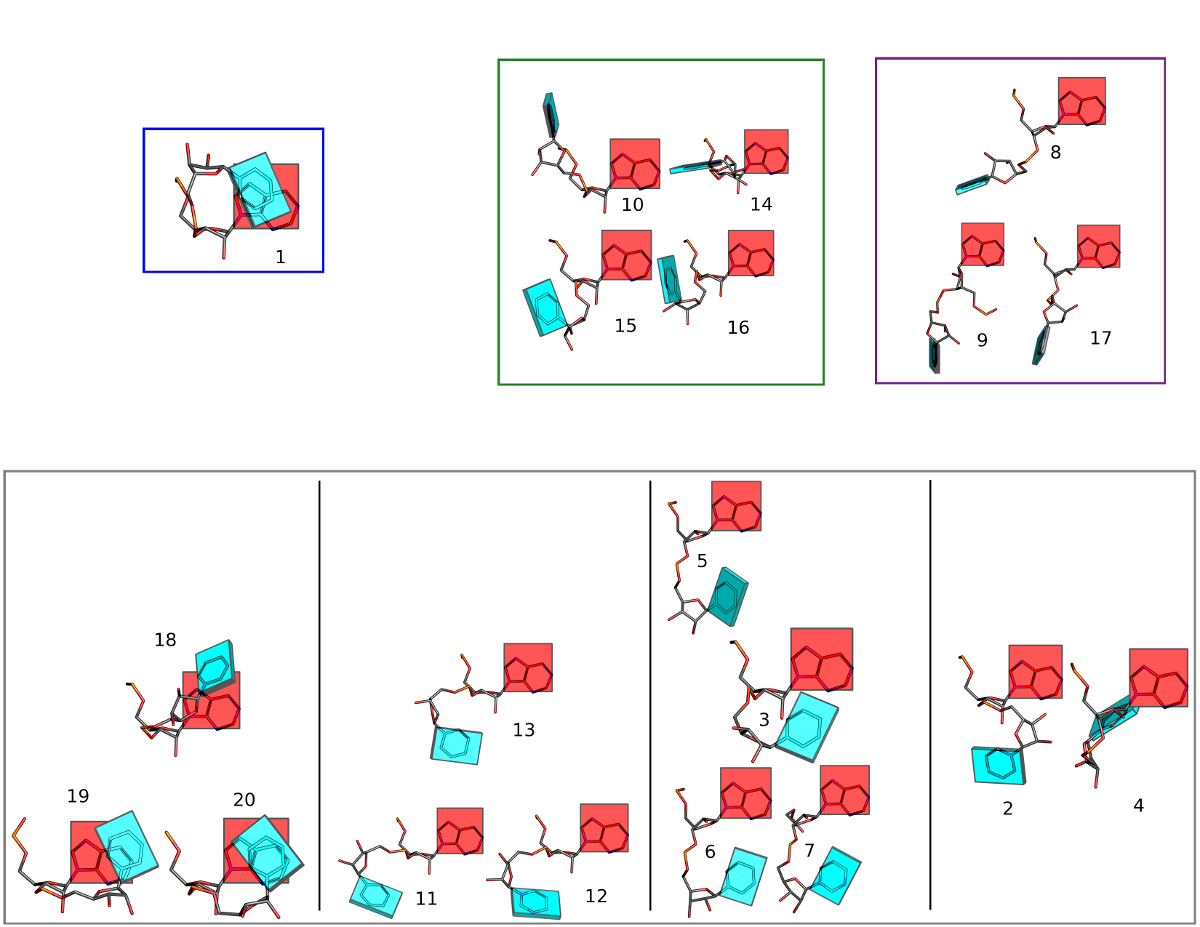
\includegraphics[angle=90, scale=0.46]{Chapter2/collageb.png}
 \caption{non-A-RNA  dinucleotide  structures  organized  by  clusters
   obtained  from   consensus  clustering  of   their  hexadimensional
   base-step parameter vectors.  The  structures have been centered on
   the reference frame  of the first step, that  is, the adenine base,
   with the minor groove edge of the rigid block on adenine facing the
   viewer.}
 \label{fig:nonAclus}
\end{figure}

As is clear  from figures~\ref{fig:nonAclus} and~\ref{fig:steps2}, the
20 identified by Schneider et  al. fall into seven unique groups based
in  the  relative position  of  base  side  groups. Group  I  contains
structure {1}  with bases stacked  and base-plane normals  pointing in
opposite   directions,   Group    II   includes   extended   unstacked
conformations  with neighboring  bases widely  displaced  and oriented
roughly perpendicular  to each other  in all cases --  structures {15,
  16, 10, 14}, Group III also contains extended conformations but with
the uracil on the minor-groove edge of adenine the bases perpendicular
to one another the uracil lies  in the "C8-carbon" of adenine in these
cases -- structures {8, 9, 17}. The bases in each of the conformers in
Group IV  are moer parallel to  one another but are  displaced in four
different  ways.   The bases  in  Group IV  a  structures  {2, 4}  are
unstacked and neither parallel nor  perpendicular. Those in Group IV b
-- structures {18, 19, 20} are  closely related to A-RNA with parallel
and stacked  bases. The bases in  group IV c, structures  {11, 12, 13}
are parallel  but unstacked  with uracil on  the major-groove  edge of
adenine. The bases  on IV d structures {3, 5, 6,  7} are also parallel
and unstacked but  with the long axis of  uracil perpendicular to that
of adenine.  As is clear from figure~\ref{fig:nonAclus} the conformers
in subgroups IV (c) and IV  (d) are closely related, and the dimers in
these two subgroups  are more closely related to  those in subgroup IV
(b) than to those in subgroup IV (a).

In order  to map back into the  23 subunit of the  ribosome the groups
which   were   obtained   by   clustering   we   have   computed   the
root-mean-square deviation (RMSD)  between the average normalized step
parameters of the  structures composing each of the  seven groups, and
the   normalized  \footnote{For  details   on  the   normalization  of
  step-parameters see Equation~\ref{eq:normalization}} step-parameters of the
2753 steps present  in the 23S subunit of  the large ribosomal subunit
(PDB\_ID:1jj2).  That  is, for  each group we  have obtained a  set of
RMSD  values  which  have  been  plotted as  histograms  as  shown  in
Figures~\ref{fig:histo1}, and~\ref{fig:histo2}.

The results are also  summarized in Table~\ref{tab:nonA}, where we can
see that they only constitute 31\% of the total amount of steps in the
23S subunit of the ribosome.  We  used a cutoff of 10 \AA \footnote{We
  retain the  traditional unit of  Angstroms to refers to  our RMSD's,
  but it  is important to  note that since  we are not refering  to an
  all-atom model such  unit does not have a  direct physical meaning.}
to select the  structures which belong to each  group, based on visual
analysis  of superimposed reconstructed  structures. For  example, for
Group I; if we reconstruct the ribosomal steps with an RMSD of 10 \AA~
or   less,  we   get  the   figure  shown   in  the   left   panel  of
Figure~\ref{fig:superimpose}. But  if we  reconstruct with the  set of
structures  with  an  RMSD  of  15  \AA~  or  less  we  start  getting
structures,  which after  being  superimposed based  on the  reference
frames of the first base are clearly not related to that group, as can
be seen in the right panel of Figure~\ref{fig:superimpose}.

We find  that the  A-RNA starting structure  kindly provided to  us by
Schneider et al. differ from canonical A-RNA in that the rise value is
4.39 \AA, rather than the  3.30 \AA~ standard value obtained for A-RNA
by Arnott and collaborators  \cite{arnott1973}. This might have affect
on the number of structures which  can be grouped under the A-RNA like
group.

Because of not getting a good representation of the total diversity of
base-steps  in the  23S  subunit of  the  ribosome, we  have opted  to
perform an  analysis based fully  on base-step parameters.  We believe
that the reason  for such poor representation is due  to the mixing of
Fourier averaging for backbones, and  the base-step perspective.
%% or it could also be  related to the fact that we  are ignoring the
%% remaining A-RNA related set of structures in Berman and
%% collaborators analysis.

\begin{table}[htbp]
\begin{center}
{\footnotesize
\begin{tabular}{c|r|c}
\hline
\bf{Group} & \bf{Percentage} & \bf{Number of Base-Steps}\\ \hline
I   & 0.11  & 3   \\ \hline
II  & 0.18  & 5  \\ \hline
III & 0.04  & 1  \\ \hline
IVa & 0.36  & 1  \\ \hline
IVb & 29.31 & 807 \\ \hline
IVc & 0.33  & 9  \\ \hline
IVd & 1.27  & 35 \\ \hline \hline
Total & 31.28 & 861   \\ \hline
\end{tabular}
}
\caption{Number of base-steps  with RMSD values less than  or equal to
  10 \AA ~between the reference  base-step vectors from the four groups
  of  non-A-type  RNA  dinucleotide  conformations and  all  base-step
  vectors found in the  23S strand of \textit{Haloarcula marismortui}.
  The  percentage  is calculated  with  respect  to  a total  of  2753
  base-steps  present in  the  23S chain  of  the 50S  subunit of  the
  ribosome.}
\label{tab:nonA}
\end{center}
\end{table}

\begin{figure}[htbp]
 \centering
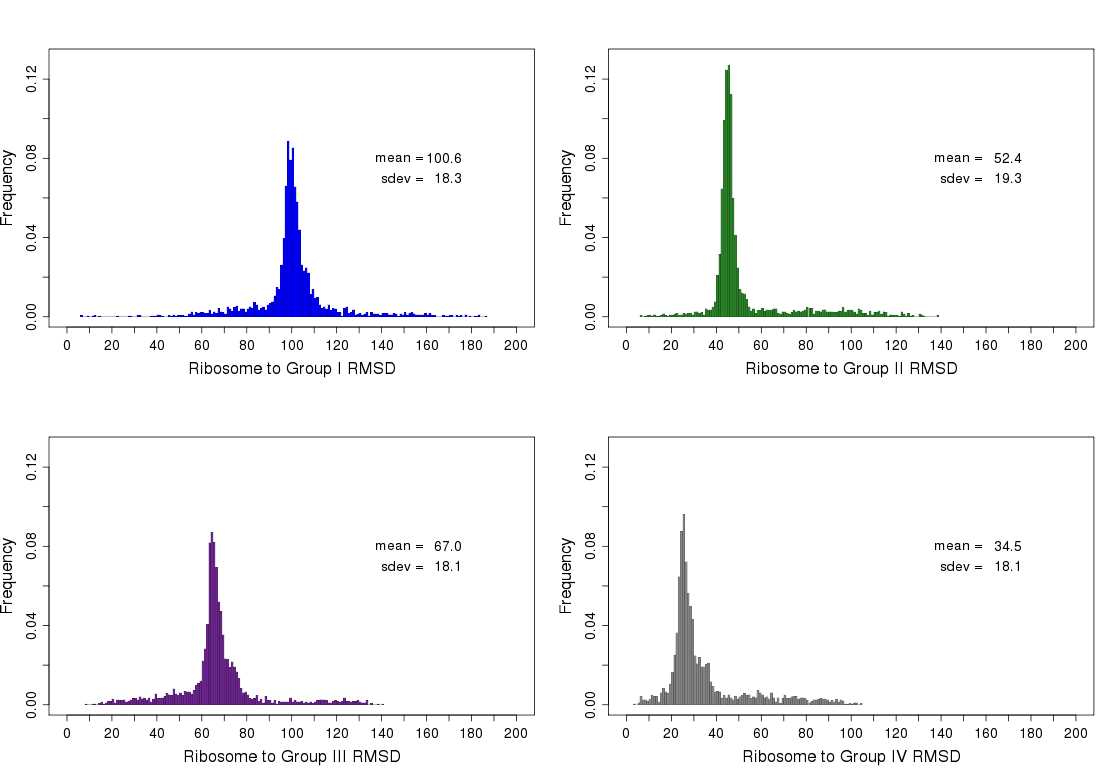
\includegraphics[angle=90, scale=0.6]{Chapter2/RMSDschneider1.png}
\caption{Root mean square deviation of the main four groups show in
  Figure~\ref{fig:nonAclus}. The color of the histograms is the same
  as that of the boxes surrounding the structures of
  Figure~\ref{fig:nonAclus}}
 \label{fig:histo1}
\end{figure}

\begin{figure}[htbp]
 \centering
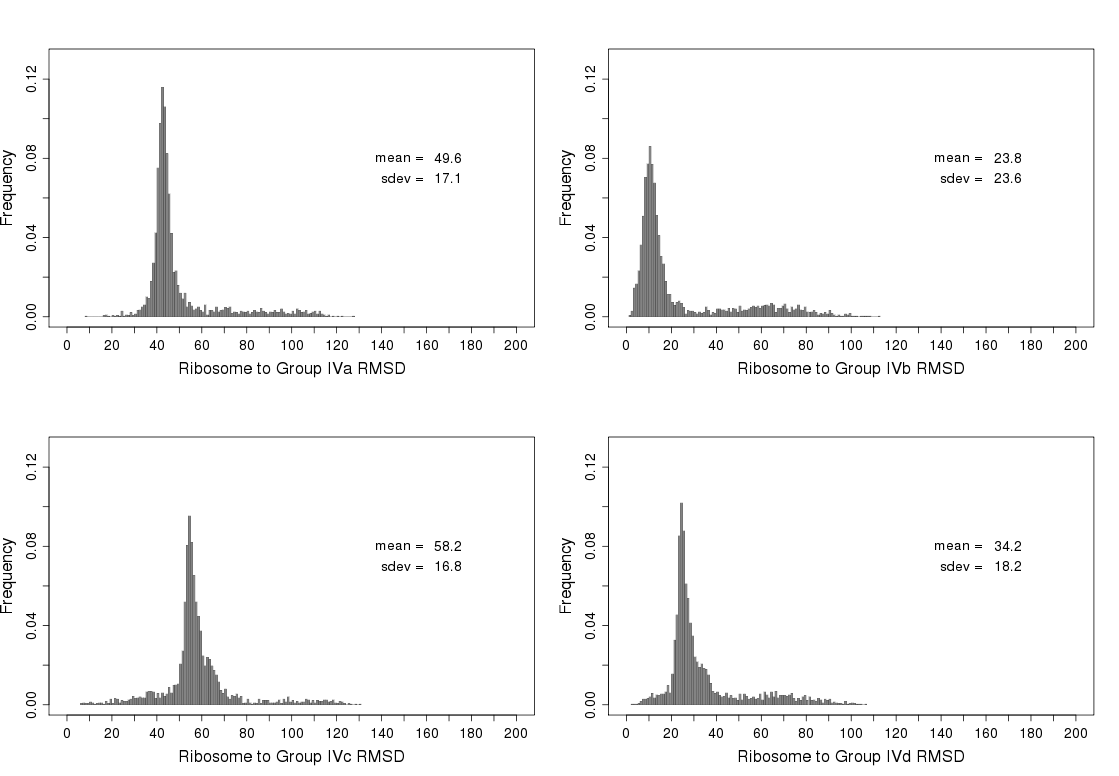
\includegraphics[angle=90, scale=0.6]{Chapter2/RMSDschneider2.png}
\caption{Root  mean  square  deviation  histograms for  the  subgroups
  present in group  IV.  Since subgroup IVb is  composed of A-RNA like
  conformations we  see in the  upper left histogram that  the highest
  proportion of small RMSD values belongs to this group.}
 \label{fig:histo2}
\end{figure}

\begin{figure}[htp]
 \centering
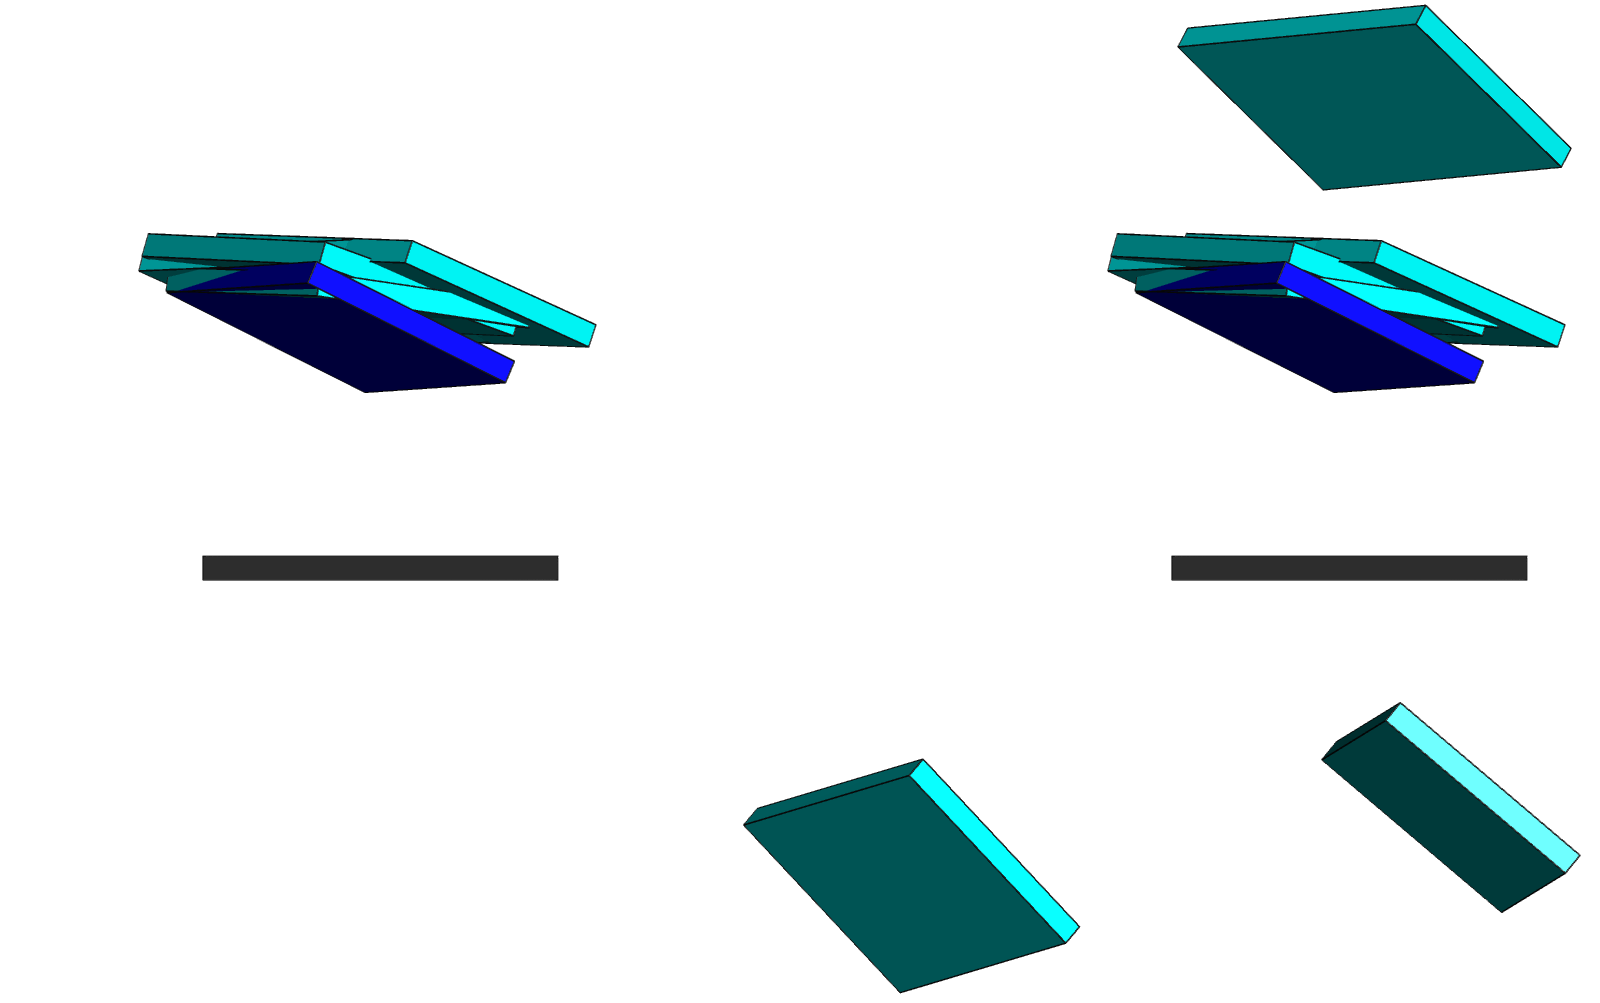
\includegraphics[angle=0, scale=0.3]{Chapter2/G1at10_15.png}
\caption{Rigid block  representation of dinucleotide  steps. The major
  groove side  of the first  nucleotide block is oriented  towards the
  viewer  and shaded  gray. \textbf{Left:}  Drawn in  blue,  the block
  representing       the        Group       I       cluster       from
  Figure~\ref{fig:nonAclus}. Superimposed  to the Group  I cluster are
  three  structures whose  step-parameter RMSD's  with respect  to the
  Group I  cluster are less than  or equal to  10 \AA. \textbf{Right}:
  With an RMSD less than or equal  to 15 \AA ~we "identify" a total of
  seven structures  from the  ribosome. We clearly  see that  three of
  them (encircled in  cyan blobs) are farther apart  from the original
  Group I  main structure of Figure~\ref{fig:nonAclus}  which is drawn
  in blue.}
 \label{fig:superimpose}
\end{figure}

\subsection{Selection of a Clustering Methodology} 
In  order to  analyze  our  dataset of  base-step  parameters we  have
decided  to  use  clustering  analysis methods.   Clustering  analysis
methods  can be broadly  classified into  two main  categories, either
partitional  or hierarchical.   In either  case the  main  problem one
faces for  classification purposes  is that of  deciding which  is the
optimal number of hierarchies or partitions that the analyzed data are
split into.  To obtain a  criterion for an optimal number of clusters,
and also  to decide which method  might be better for  our dataset, we
have used two types  of cluster-validation techniques.  They are known
as  internal measures  and stability  measures.  Full  details  of the
definitions  of   such  measures  are   provided  in  \cite{handl2005,
brock2008} and  Appendix~\ref{appendix_c}.  To perform  the validation
analysis  we   used  a  cluster  validation   package  called  clValid
\cite{brock2008},   which  is  implemented   in  the   R  \cite{rcite}
statistical analysis package.

In  Figures~\ref{fig:internal} and~\ref{fig:stability} we  present the
results  for  internal  and  stability  validation  of  the  base-step
parameters  in  the  23S  ribosomal  subunit.  In  clustering  anlysis
literature it is customary to use  a variable $k$ to define the number
of clusters.

We computed  the validation  scores for a  number of  clusters ranging
from  $k=2$, up  to $k=80$,  and evaluated  both  hierarchical methods
(hierarchical, diana)  and partitional (kmeans, pam,  som, sota).  The
connectivity  measure must  be minimized,  and the  average silhouette
width  (silhoutte) and  Dunn index  must be  maximized.  With  this in
mind,  we see  that the  hierarchical\footnote{The  hierarchical label
  refers  precisely to  the agglomerative  (bottom-up)  technique, the
  Euclidean metric, and the average method.} method performs better in
connectivity and  dunn index for the  whole range, and it  is also the
best performer in silhoutte from $k=12$ onwards.

Stability measures  (~\ref{fig:stability}) are well  suited for highly
correlated data sets with linear correlation between variables, but
they are not very useful for our data set,
which show  only such correlation in  shift and twist, as  can be seen
from  the values on  the upper  right corner  of the  pairs scatteplot
shown  in   Figure~\ref{fig:pairsnoarna}.   We  include   the  cluster
stability measures for completeness.

\begin{figure}
 \centering
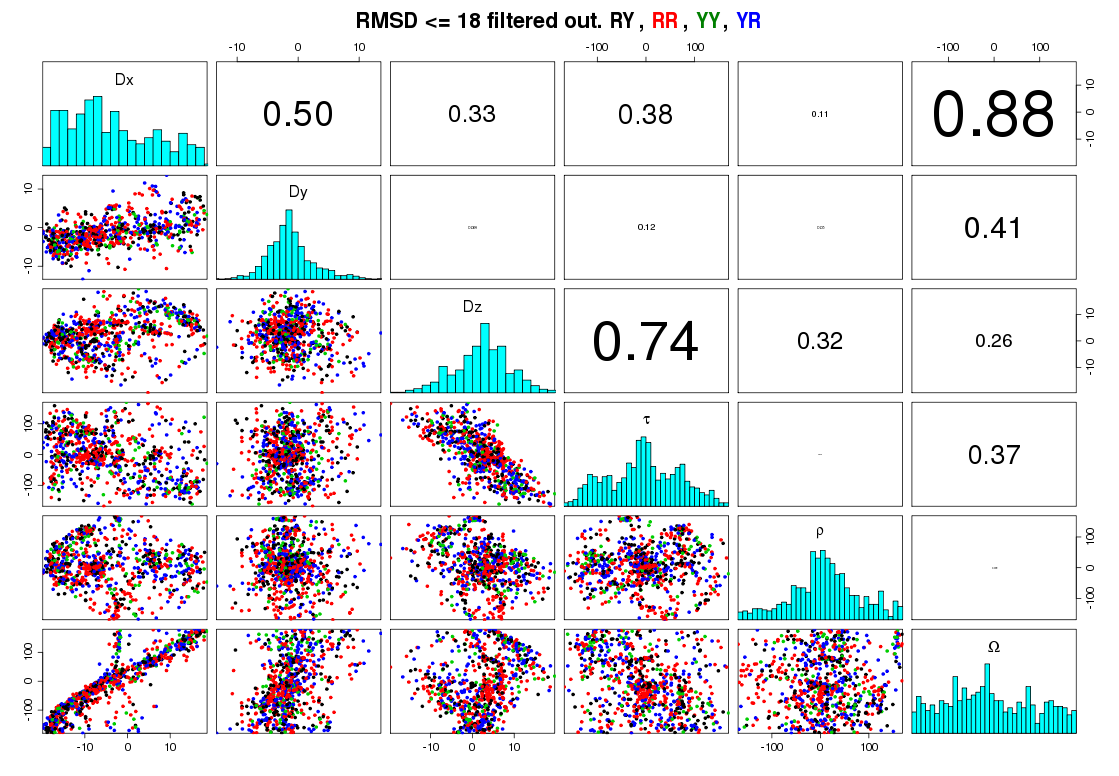
\includegraphics[angle=90, scale=0.5]{Chapter2/noarna_step.png}
\caption{Pairs  scatterplot for  base-step  parameters, shift,  slide,
rise,  tilt,  roll,  and  twist,  for the  non-A-RNA  dataset  colored
according   to   purine-pyrimidine   (black),   purine-purine   (red),
pyrimidine-pyrimidine    (green),    and   pyrimidine-purine    (blue)
steps. Here  the correlation coefficients of each  of the scatterplots
shown in the lower half of the graph are listed in the mirror position
in  the upper  half of  the  diagram, i.e.,  the shift-twist  ($D_{x},
\Omega$) correlation  coefficient (0.88) of the plotted  data shown in
the lower left corner, is printed in the upper right corner.}
 \label{fig:pairsnoarna}
\end{figure}

The stability measurements  we have computed are read  as being better
the smaller their values, of  these. We have determined three measures
for  each of  the hierarchical  and partitional  methods,  namely, the
average proportion  of non-overlap  (APN), the average  distance (AD),
and  the average  distance between  means (ADM).   The detail  of such
measures  is given  in Brock  et  al.  \cite{brock2008}.   As seen  in
Figure~\ref{fig:stability} the method with the best stability measures
is sota for APN  and ADM almost for the whole range,  up to ~ 70.  For
the AD  measure the best  performers are pam  and sota over  the whole
range.  Notice that the hierarchical  method follows the same trend as
the other methods, and that in general, apart from the APN measure and
the sota  method, all  methods exhibit a  similar behavior due  to the
fact that our data set is  not highly correlated. That is, the dataset
cannot be split into a few principal components.

In all cases  we also see that the best overall  number of clusters is
two, which is not surprising since we haven't filtered out A-RNA
structures from our  data set. The two main  groups are A-RNA
type base-steps, and non-A-RNA steps.

\begin{figure}
 \centering
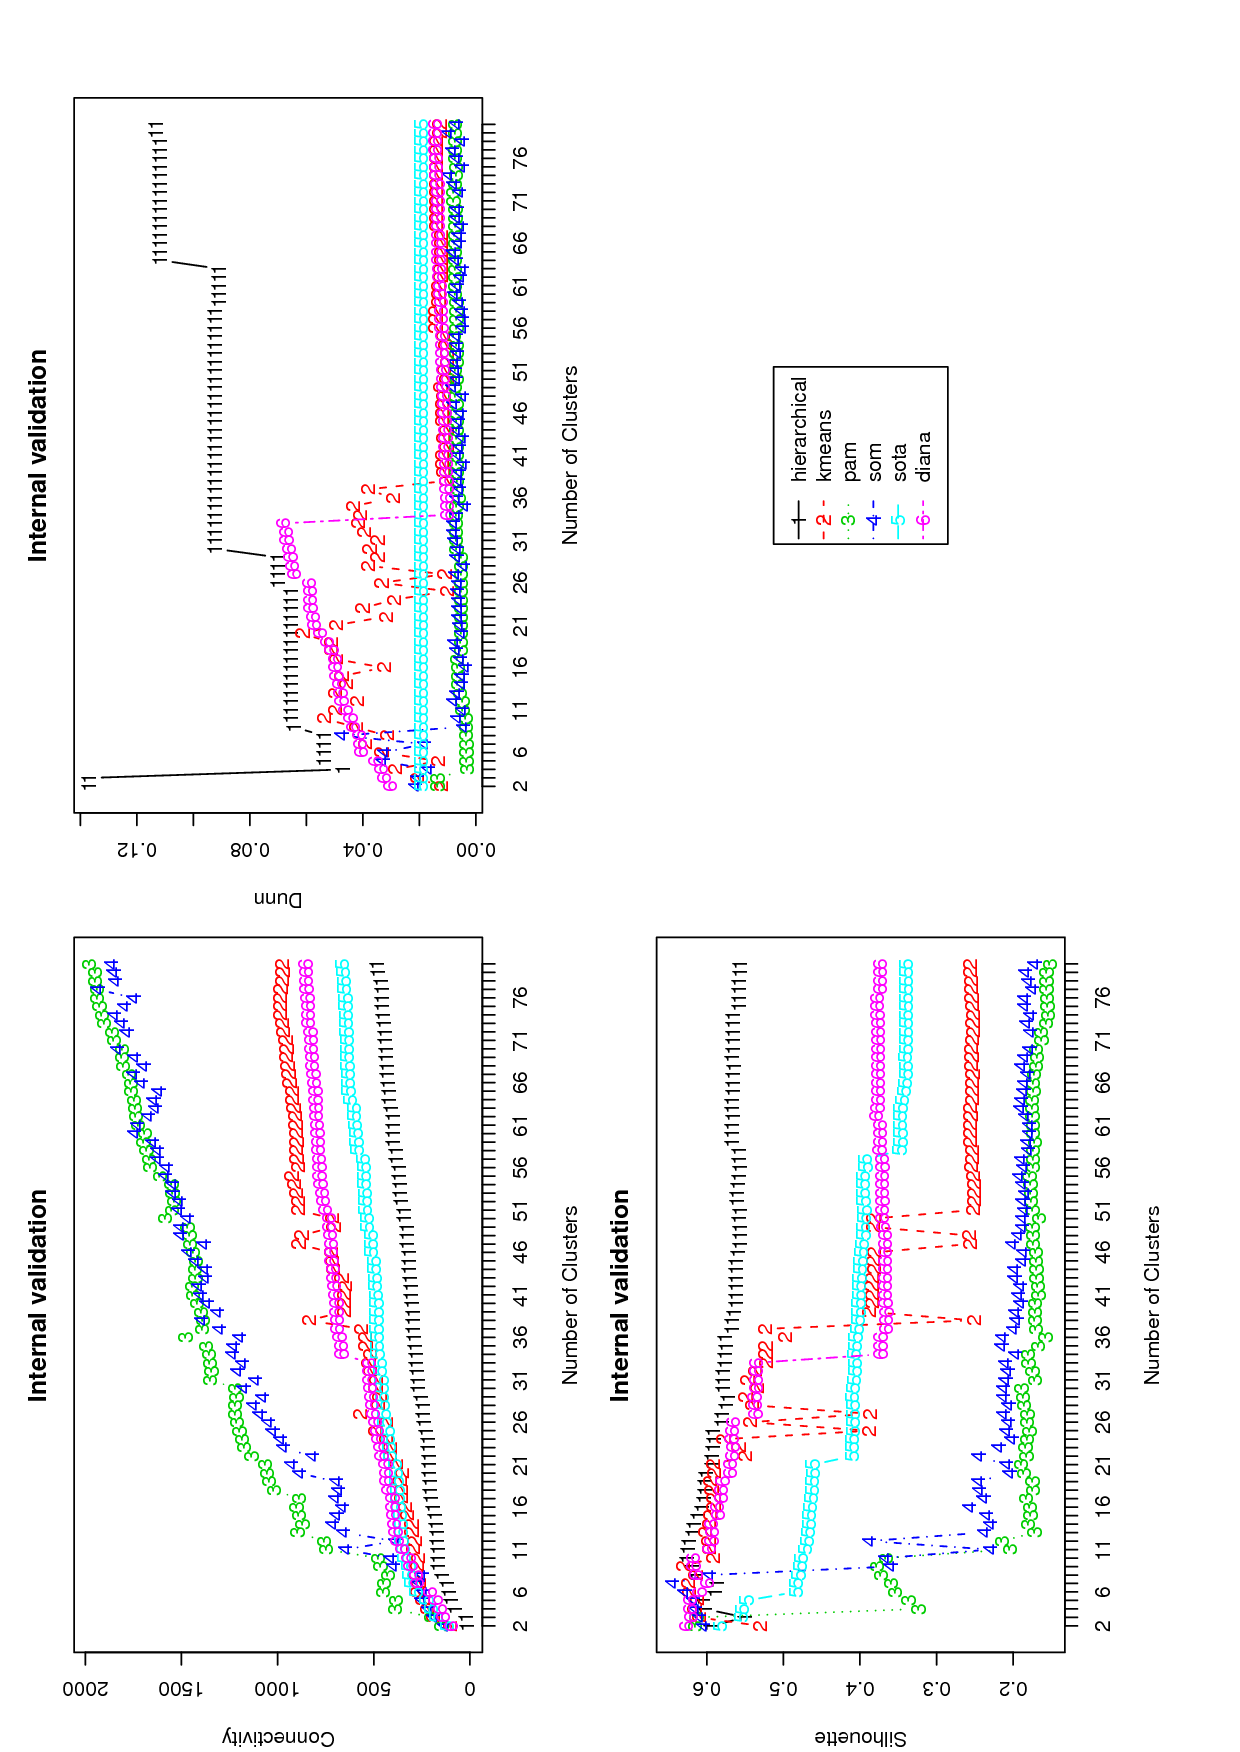
\includegraphics[angle=0, scale=0.38]{Chapter2/STval_int.png}
\caption{Cluster validity scores for internal measures. Notice how the
  hierarchical method, labeled as 1 in black color,
  behaves better for the whole range of Connectivity (smaller values)
  and Dunn (higher values),
  and it also outperforms all others after $k=12$ for Silhoutte
  (higher values) scores.}
 \label{fig:internal}
\end{figure}

\begin{figure}
 \centering
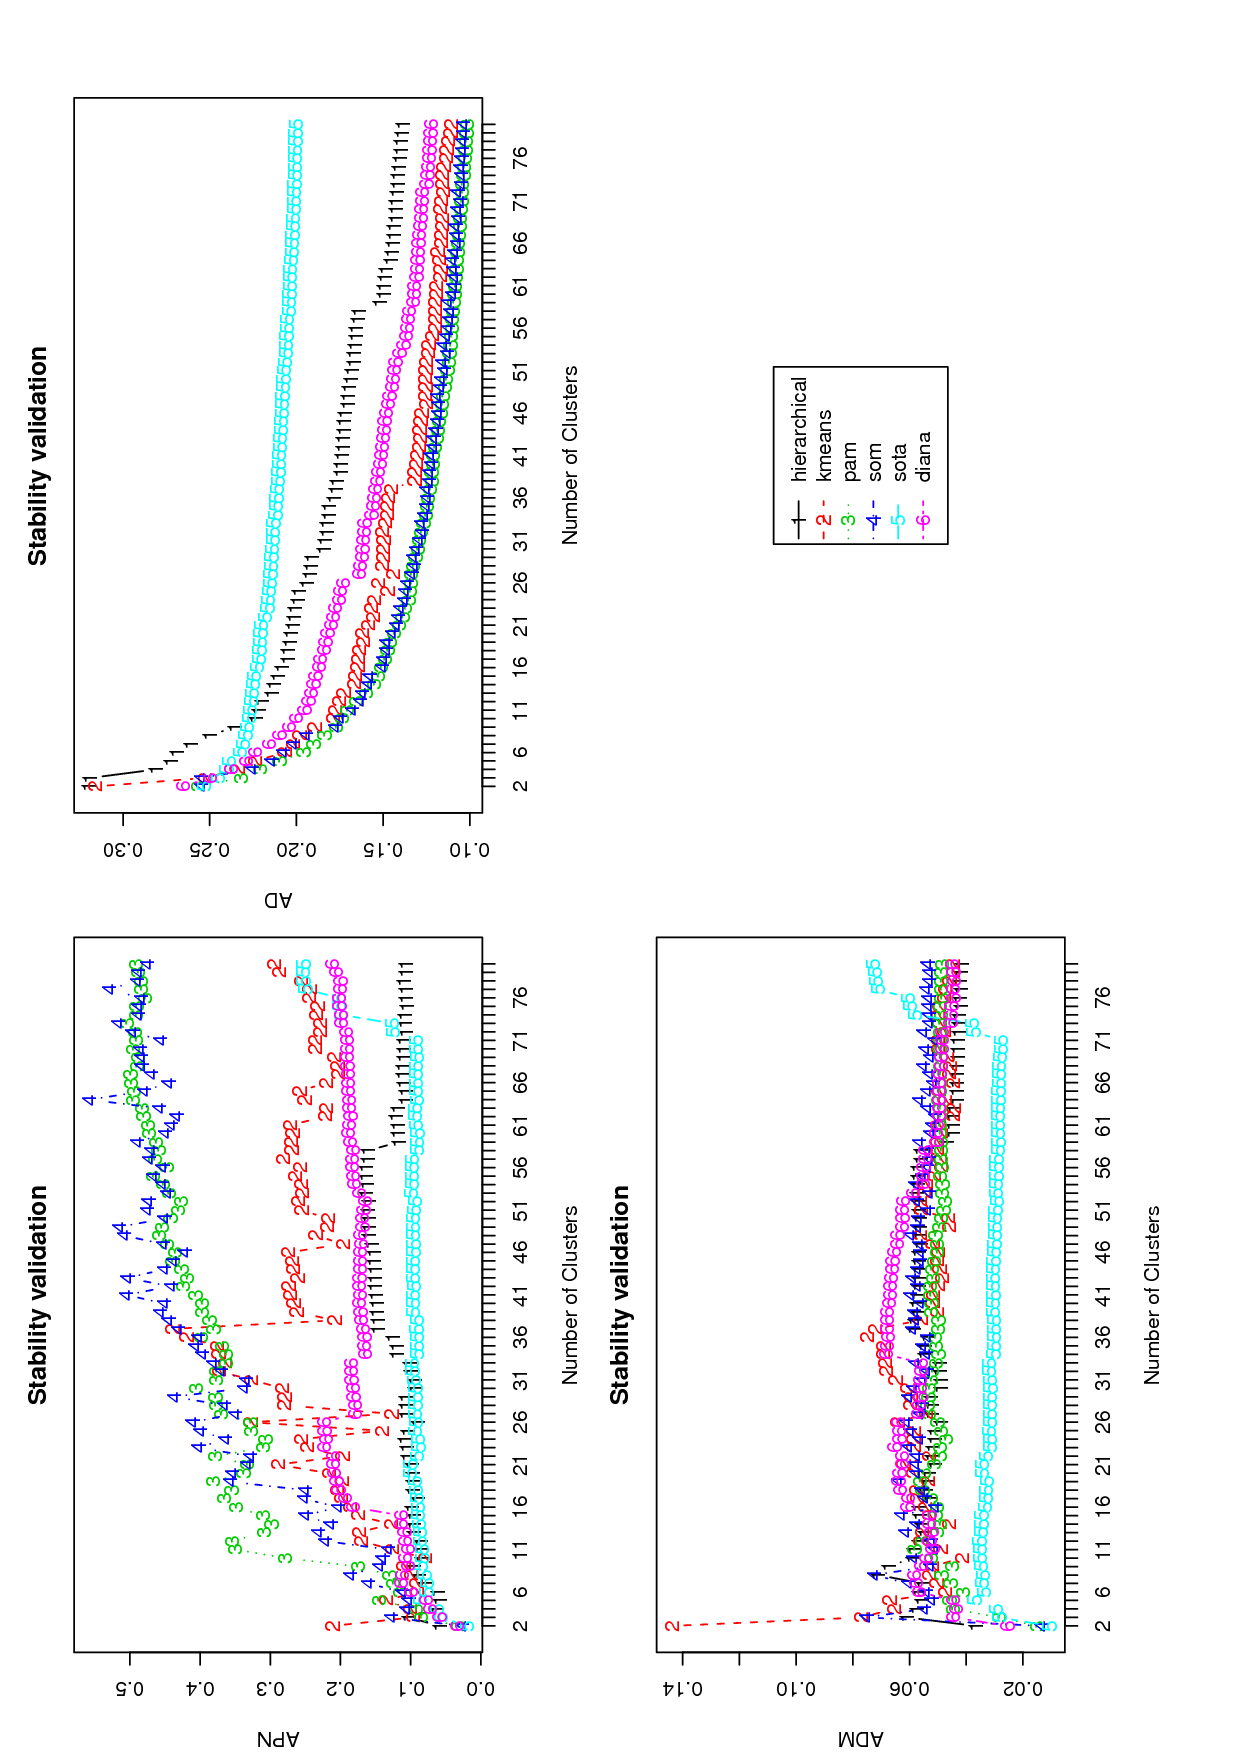
\includegraphics[angle=0, scale=0.38]{Chapter2/STval_sta.png}
\caption{Cluster validity scores for stability measures.}
 \label{fig:stability}
\end{figure}

We focus  our attention on the  group of structures  which differ from
A-RNA.  We have  extracted 797  such steps  (about 29\%  of  the total
number  of steps)  from  the  dataset based  on  the root-mean  square
deviation  between  step  parameters (Figure~\ref{fig:dormsd}).  These
base-step parameters are  those with RMSD values greater  than 18 \AA.
These RMSD values have  been computed between the base-step parameters
of  23S  RNA  and  the  standard base-step  parameter  values  of  the
canonical   A-RNA  helix  determined   by  Arnott   and  collaborators
\cite{arnott1973}  work. The standard  base-step parameter  values for
common    double-stranded    RNA     and    DNA    are    listed    in
Table~\ref{tab:conformations}.

\begin{figure}
 \centering
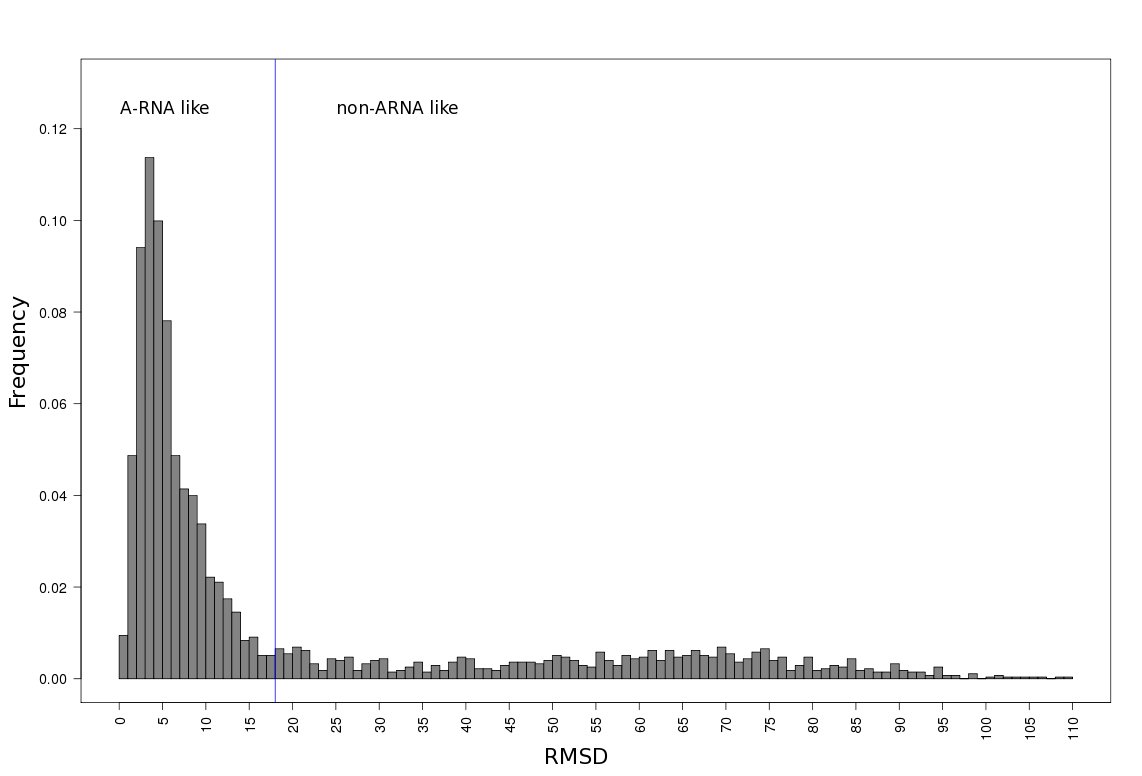
\includegraphics[angle=0, scale=0.3]{Chapter2/dormsd.png}
\caption{RMSD values between base-step parameters of the 23S subunit of
  ribosomal RNA and the standard base-step parameters derived from
  Arnott and collaborators \cite{arnott1973} work.}
 \label{fig:dormsd}
\end{figure}

\begin{table}
\begin{center}
{\small
\begin{tabular}{p{2cm}|c|c|c|c|c|c|c|c}
\hline
\textbf{Structure Name} & Shift ($D_x$) & Slide ($D_y$) & Rise ($D_z$) & Tilt
($\tau$) & Roll ($\rho$) & Twist ($\Omega$) & \textbf{Reference} &
Method \\ \hline
A-DNA & 0.36 & -1.39 & 3.29 & 2.46 & 12.50 & 30.19 & Arnott
\cite{arnott1999} & fiber-diffraction \\ \hline
B-DNA & 0.44 & 0.47 & 3.33 & 4.63 & 1.77 & 35.67   & Arnott
\cite{arnott1999} & fiber-diffraction \\ \hline
A-RNA & -0.08 & -1.48 & 3.30 & -0.43 & 8.64 & 31.57 & Arnott
\cite{arnott1999} & fiber-diffraction \\ \hline
A'-RNA & 0.05 & -1.88 & 3.39 & -0.12 & 5.43 & 29.52 & Arnott
\cite{arnott1999} & fiber-diffraction \\ \hline
AII-RNA & 1.01 & -2.52 & 3.33 & 2.94 & 9.75 & 25.12 & Schneider
\cite{schneider2004} & X-ray \\ \hline
\end{tabular}
}
\caption{Base step parameters for common DNA and RNA
  conformations. The base-step parameters are computed for
  a single-stranded base-step rather than a double-stranded base-pair step.}
\end{center}
\label{tab:conformations}
\end{table}

With the filtered dataset, which we refer to as the non-A-RNA dataset,
we  have repeated  the cluster  validation analysis  for  the internal
measures  (Figure~\ref{fig:noarna}). From this  analysis we  see again
that the  best method for  clustering our dataset is  the hierarchical
method. The Dunn index, which works under the idea of finding the best
possible separation  and compactness  between clusters, shows  us that
the optimal number of clusters  is $k=67$. The other two indices show,
as for the whole dataset case,  that the optimal number of clusters is
two, nonetheless, a common  indicative of optimal cluster solutions in
the  connectivity and  silhouette plots  is given  by the  presence of
shoulders.  We  see that there  is a shoulder  also at $k=67$  for the
connectivity and  silhouette plots. We selected the  67 clusters given
by   the   hierarchical   method,   and   took   their   corresponding
step-parameter values to  reconstruct the dinucleotide step structures
using 3DNA.  In Figure~\ref{fig:noarnak67} we draw the first seventeen
groups with  ten or more structures,  which account for  80 percent of
the  non-A-RNA steps.   We  also plot  in  the lower  right corner  of
Figure~\ref{fig:noarnak67} the  set of 20 structures  derived from the
work  of Schneider et  al.\cite{schneider2004}, and  the whole  set of
non-A-RNA  dinucleotide  steps in  a  common  reference  frame on  the
adenine  of  an ApU  step.   All  structures  are centered  using  the
standard  reference frame  embeded in  the  first base,  which in  our
reconstructions corresponds to a red block representing adenine, whose
minor groove  edge is oriented to  the left, its major  groove edge is
oriented  to the  right, and  its so-called  Watson-Crick base-pairing
edge is pointing towards the viewer.

When comparing the 17 groups of non-ARNA dinucleotide steps with those
coming from  the work  of Schneider and  collaborators we see  that in
their set  of structures there are  no steps represented  at the major
groove side of the red  block representing adenine, that is, the right
side of  the red adenine block. We  also see, that even  though the 17
groups represented are not as  compact as one would desire, they start
to  give an  indication of  geometrical  preferences on  the space  of
dinucleotide step-parameters.  For example, it is remarkable to see in
group  7, labeled  as  g7.png in  Figure~\ref{fig:noarnak67} that  the
blocks  representing  uracyl  in   cyan  color,  orient  their  planes
orthogonally to  the major groove  side of the red  block representing
adenine.

The reason we choose to  include the figure of all non-ARNA base-steps
in Figure~\ref{fig:noarnak67} is that of  giving the reader an idea of
the complexity of the  space of base-step conformations described from
a  base  viewed  perspective  instead  of  the  more  common  backbone
perspective, this also suggests that the task of finding order in this
broad range of possible conformations is analog to the task of peeling
an onion. We believe the onion can be effectively peeled into parts by
using  appropriate validated clustering  analysis techniques.

\begin{figure}
 \centering
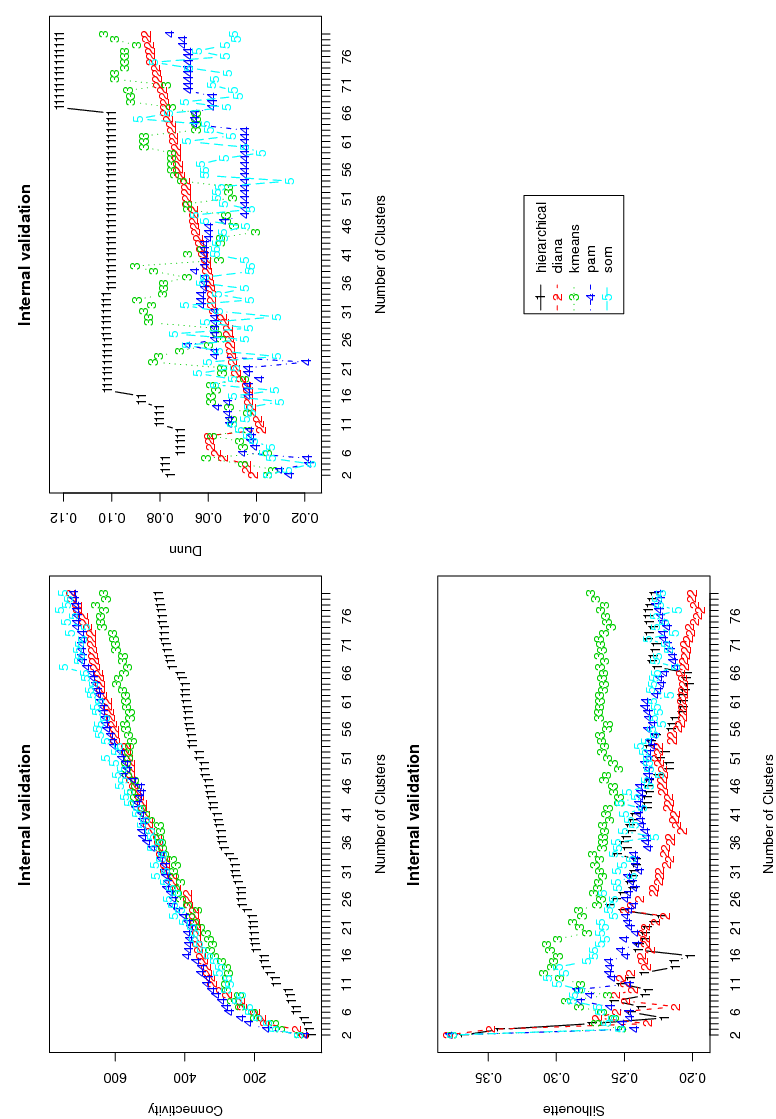
\includegraphics[angle=0, scale=0.9]{Chapter2/noarna_val.png}
\caption{Cluster validity  scores for the non-ARNA dataset.  It can be
  seen  clearly  that  the   optimal  method  for  clustering  is  the
  hierarchical one,  as measured by  lower values in  the connectivity
  scores, and higher  values in the Dunn score.  The optimal number of
  clusters given  by the dunn  score is 67,  we also see  shoulders at
  $k=67$, for the connectivity and silhouette scores.}
 \label{fig:noarna}
\end{figure}

\begin{figure}
\centering
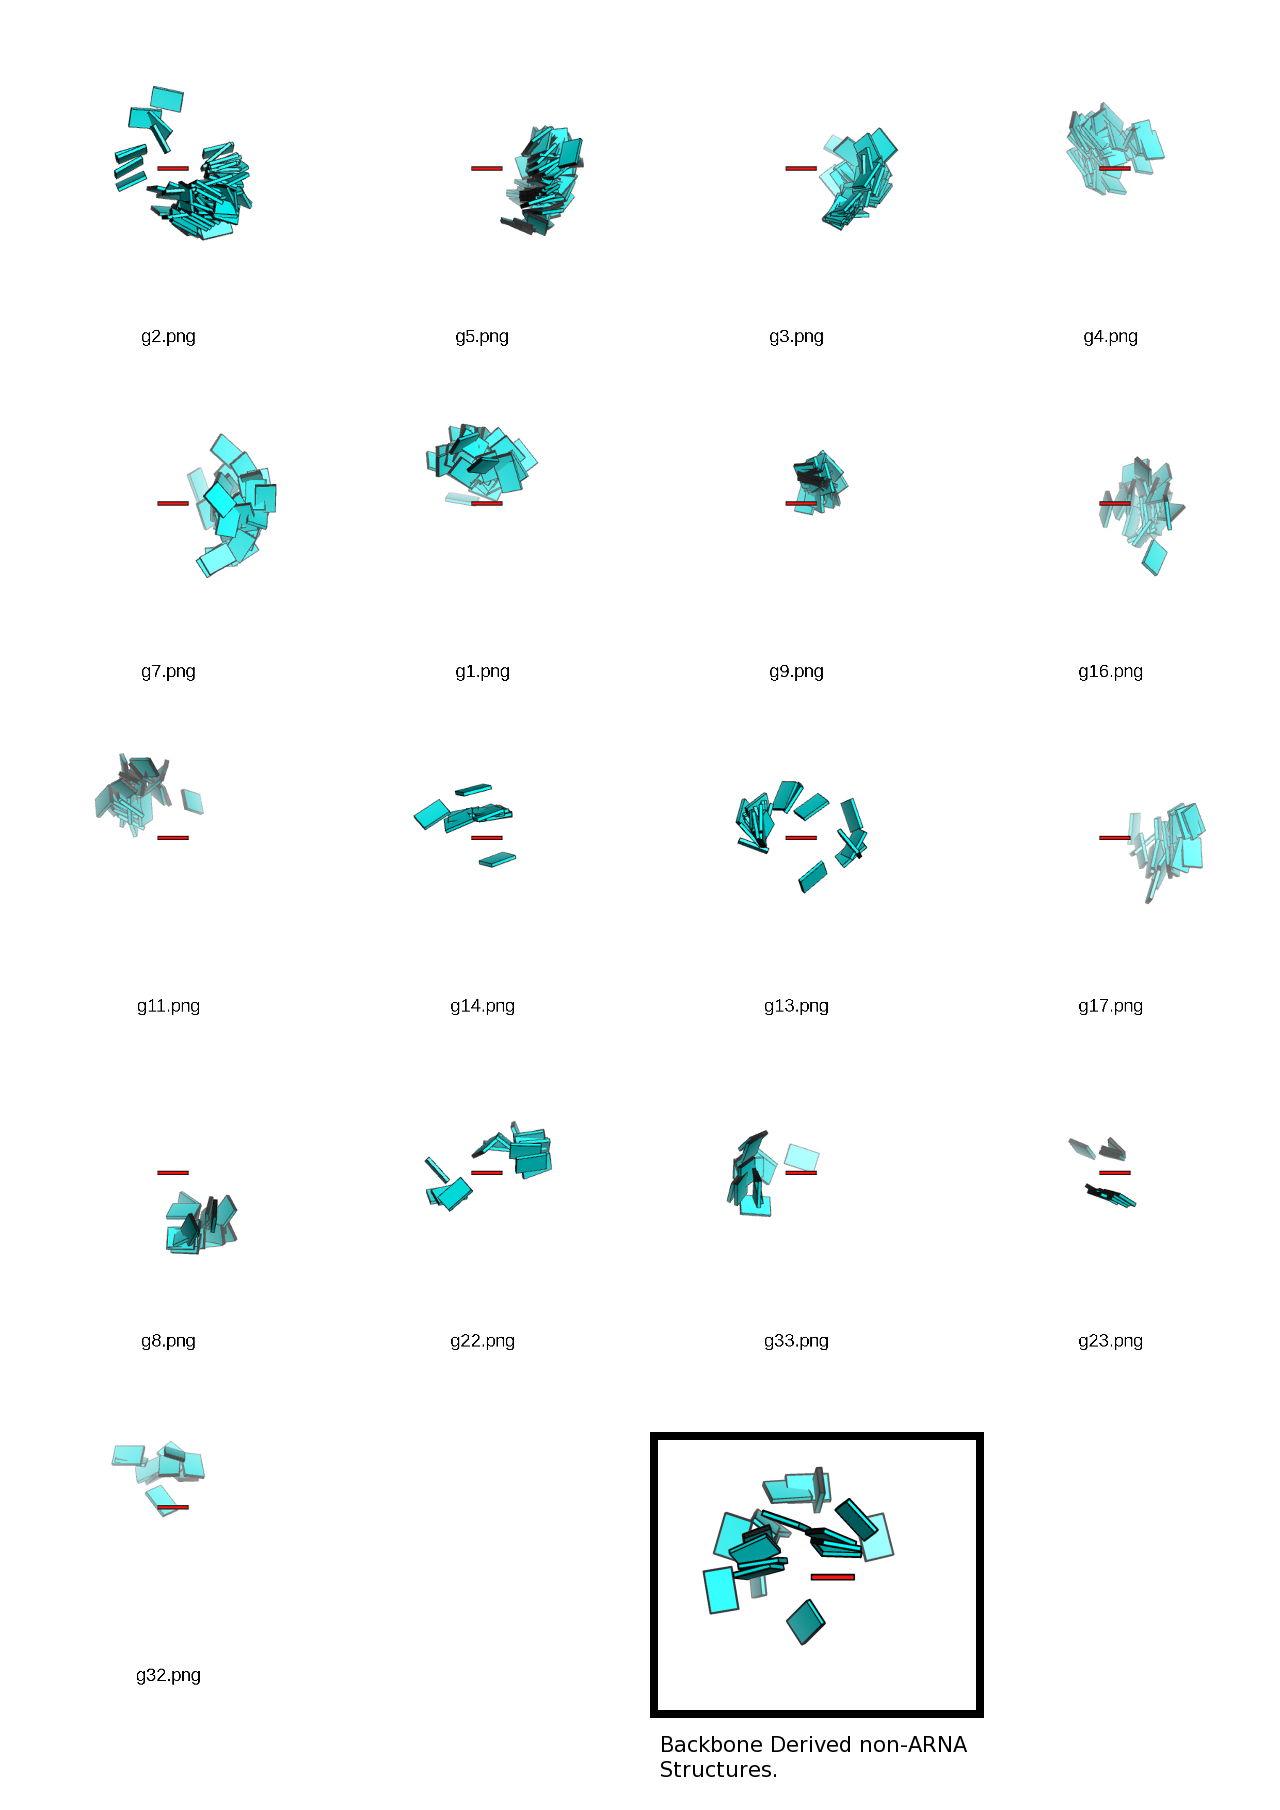
\includegraphics[angle=0, scale=0.35]{Chapter2/k67_17.png}
\caption{17  out of  the 67  groups clustered  using  the hierarchical
  clustering  algorithm  are  drawn  in  a  photograph  contact  sheet
  fashion. Each group  is centered on the base  reference frame of the
  adenine  block  drawn in  red.  In the  lower  right  corner of  the
  "contact sheet" the full space  of 797 reconstructed steps is shown,
  along with the  20 steps derived from schneider  et al. work. Notice
  how the only "hollow" side of the "onion" formed by the full space of
  base-step  conformations is that  corresponding to  the Watson-Crick
  base-pairing edge.}
\label{fig:noarnak67}
\end{figure}



\bibliography{biblio}


\chapter{RNA Base-Pairing}
\label{basepairs} 
\bibliographystyle{nar}
\section{Canonical and Noncanonical Base-pairs}
As  shown   in  Figure  \ref{fig:saenger28},  there   can  be  various
base-pairing patterns between heterocyclic  bases in nucleic acids due
to the  variety of possible  hydrogen bonding interactions.   The most
prevalent  hydrogen   bonding  pattern   is  that  of   the  canonical
Watson-Crick  base-pair.  All  other  possible patterns  are known  as
non-canonical base-pairs and  are more common in RNA  than in DNA.  We
used the 3DNA \cite{lu2003} software package to find all base-pairs in
a  non-redundant   dataset  of   RNA  structures  obtained   by  X-ray
crystallography with  resolution better  than 3.5 \AA  downloaded from
the  protein data  bank  (PDB).   We also  constrained  our search  to
helical regions defined as having three consecutive base-pairs or more
which need  not be covalently  bonded by the  sugar-phosphate backbone
between consecutive base-pairs \cite{olson2009}.

Our database is  non-redundant in the sense that  from the main source
of RNA structural information, which is the ribosome, we used only one
of the  available structures  per organism, that  is, one for  each of
\textit{Deinococus   radiodurans},   \textit{Haloarcula  marismortui},
\textit{Escherichi          coli},         and         \textit{Thermus
  thermophilus}. Table~\ref{tab:dbase}  shows in detail  the number of
bases per RNA type.
\begin{table}[htbp]
\begin{center}
\begin{tabular}{|l|c|r|r|r|r|}
\hline
RNA Type & \multicolumn{1}{p{2cm}|}{Number of Structures} & \multicolumn{1}{c|}{G} &
\multicolumn{1}{c|}{C} & \multicolumn{1}{c|}{A} &
\multicolumn{1}{c|}{U} \\ \hline \hline
small helices & 78 & 891 & 753 & 404 & 442 \\ \hline
drug-RNA & 36 & 932 & 862 & 365 & 433 \\ \hline
protein-RNA & 207 & 4001 & 3457 & 1771 & 1731 \\ \hline
protein-tRNA & 9 & 175 & 155 & 98 & 87 \\ \hline
rRNA & 13 & 3866 & 2949 & 1939 & 1785 \\ \hline
tRNA & 13 & 205 & 159 & 124 & 112 \\ \hline
ribozyme & 113 & 2434 & 2086 & 1438 & 1150 \\ \hline
Total & 469 & \multicolumn{1}{c|}{12504} & \multicolumn{1}{c|}{10421} & \multicolumn{1}{c|}{6139} & \multicolumn{1}{c|}{5740} \\ \hline
\end{tabular}
\caption{Classification of RNA Types in Non-Redundant Dataset at less
  than 3.5 \AA~(For Base-Pairs in Helices of 3 base-pairs or more).}
\label{tab:dbase}
\end{center}
\end{table}



In the helical regions data we quantify:

Abundances (Counts)
Deformabilites
Helical Context




\section{Clustering of Yurong's Classification}

\bibliography{biblio}


\chapter{RNA Base Pair Steps}
\label{basepairsteps} 
\bibliographystyle{nar}
Before  the turn  of the  century it  was still  not  conceivable that
knowledge-based potentials  could be obtained for  RNA helical regions
due to the  small amount of crystallographic data  available. This was
not the case  for DNA, where enough data for  such potentials has been
available   since   1998  as   shown   by   Olson  and   collaborators
\cite{olson1998}.   As  pointed  out  in  Chapter  2,  the  number  of
high-resolution X-ray  crystal structures of RNA has  increased by two
orders of magnitude, giving us enough information to develop a dimeric
model of double-helical  RNA with 10 unique base-pair  steps formed by
the canonical G$\cdot$C and  A$\cdot$U Watson-Crick pairs. An extended
model with 21  unique dimeric steps can also  be constructed by adding
the wobble G$\cdot$U base-pair  to canonical G$\cdot$C, and A$\cdot$U,
but for the GU$\cdot$GU (11  cases) and UA$\cdot$UG (20 cases) dimeric
data is still  scarce. An illustration of the  possible unique dimeric
steps which can be formed in RNA as mentioned above is given in Figure
\ref{fig:unique}.

\begin{figure}
\centering
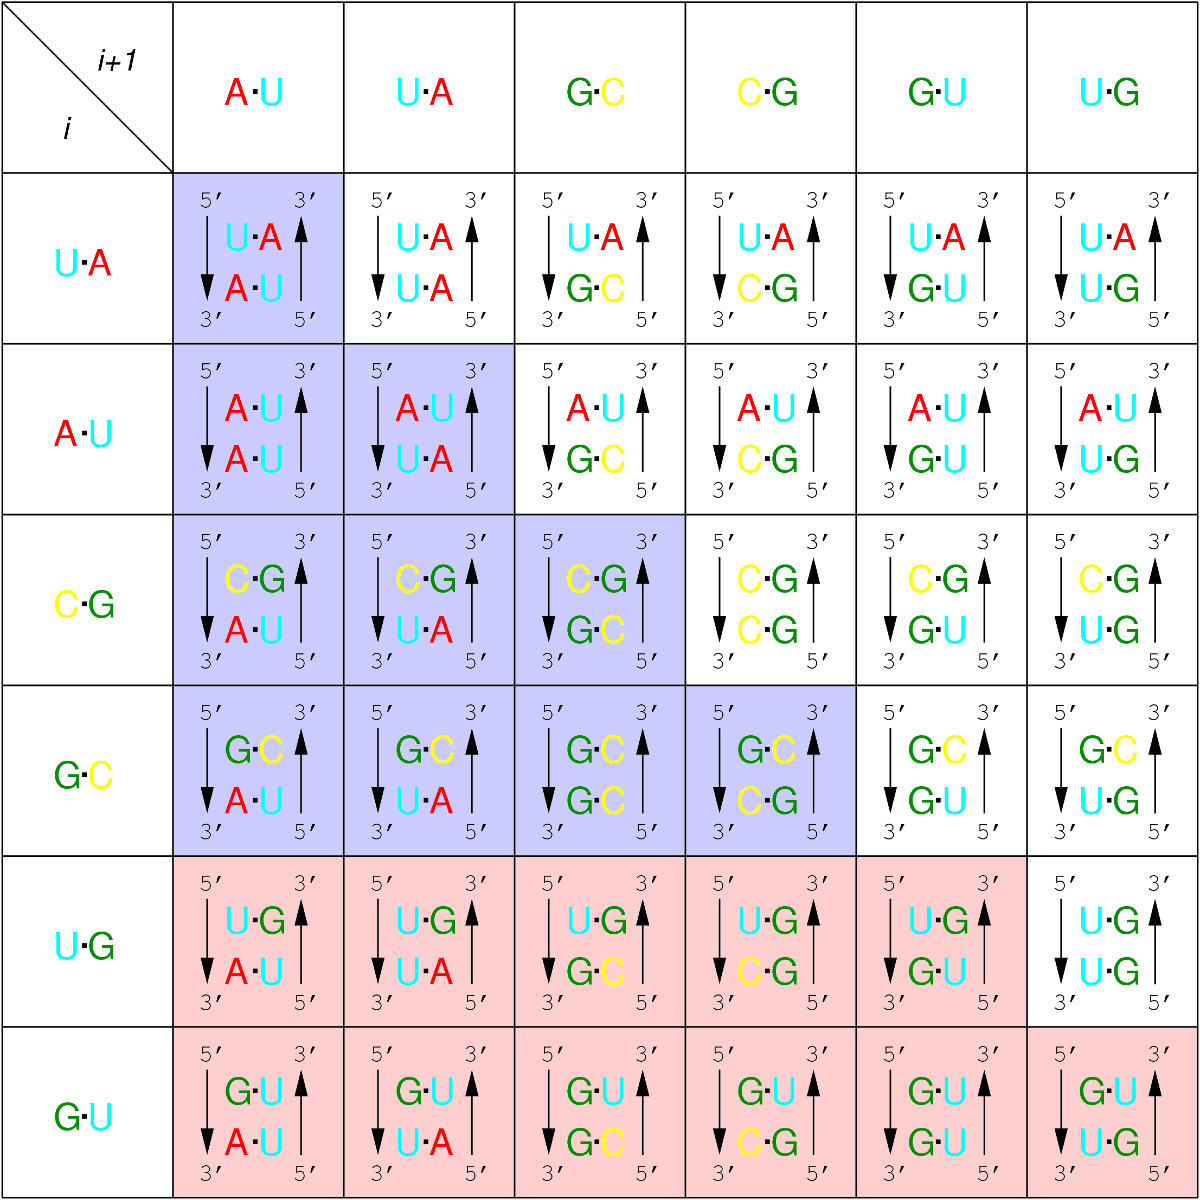
\includegraphics[angle=0, scale=0.4]{Chapter4/unique.png}
\caption{Unique base-pair dimers of RNA formed by canonical G$\cdot$C,
  canonical    A$\cdot$U    Watson-Crick,    and   wobble    G$\cdot$U
  base-pairs.  In purple  boxes the  10 unique  base-pair steps
  formed  by canonical G$\cdot$C  and A$\cdot$U,  and in  beige boxes
  the  additional  11   base-pair  steps  which   result  from
  considering G$\cdot$U  wobble base-pairs as dimer  building block to
  give a total of 21 unique  dimers. The coloring scheme used to color
  the bases is that  used in the NDB, where A is red,  U is cyan, G is
  green, and C is yellow. The first  base-pair in the step in the 5' to
  3' sense is  identified as pair $i$ and the  second is identified by
  $i+1$ as shown in the upper left corner of this figure.}
\label{fig:unique}
\end{figure}  

For the  case of the possible  91 unique base-pair steps  which can be
formed from the seven  dominant base-pairing types discussed in Chapter
3,  we see tendencies of favoured sequences infered from counts of the
available data as will be shown in the next section. 

The results obtained from  the analysis of RNA knowledge-based dimeric
information allow us to explore RNA at the global level, that is, as a
polymer  chain. Therefore we can compute  the  persistence  length  of
some  RNA sequences as shown in the last section of this chapter.

\section{Base-Pair-Steps in Intact Helical Regions}
From  the  dataset  of  base-pairs  described in  Chapter  2  we  also
collected base-pair step information  and focused our attention in the
dimers which are  located in intact helical regions,  those noted as H
in  Figure   \ref{fig:helregxin}.   From  the  data   shown  in  Table
\ref{tab:91steps}  we see that  it's more  common for  a non-canonical
base-pair   to  partner  up   with  a   canonical  base-pair   than  a
non-canonical  one.  The  number of  steps formed  by  a non-canonical
base-pair and a  canonical one is six times higher  than that of steps
formed  by  two non-canonical  pairs.   Some non-canonical  base-pairs
occur exclusively in  the context of a stack  of non-canonicals, e.g.,
GA$_{s}$$\cdot$GA$_{s}$, where two  sheared base-pairs stack together,
or also  on stacks  of a sheared  G$\cdot$A base-pair and  a Hoogsteen
A$\cdot$U  base-pair.  The  majority of  stacks  between non-canonical
base-pairs  occurs  on  dimeric  steps  composed  of  combinations  of
G$\cdot$U  wobble  and  sheared  G$\cdot$A  base-pairs.   Overall  the
majority  of dimeric  steps are  those formed  by  canonical G$\cdot$C
base-pairs  making up  more than  a third  of the  whole.  It  is also
interesting that  more than half  of this kind  of steps is  formed by
GG$\cdot$CC steps.

Overlap values between base-pairs  are given in parentheses along with
the  counts  of dimeric  steps  in  intact  helical regions  in  Table
\ref{tab:91steps}. Looking  at these values the common  trend seen for
overlaps of DNA base-pairs  is mantained, i.e., purine-pyrimidine (RY)
steps have the greatest overlap values, and pyrimidine-purine (YR) the
smallest.   When   the  G$\cdot$U  wobble  base-pair   is  taken  into
consideration the trend remains  true, but the values are considerably
increased, for example for the  GU$\cdot$GU dimer the overlap value is
14.4 \AA$^{\text{2}}$.   The other values  which show a  large overlap
are those of the dimers  composed of sheared G$\cdot$A pairs and those
composed  of sheared G$\cdot$A  and U$\cdot$U  wobble.  The  degree of
overlap doesn't necesarily correlate with greater dimer stabilities as
judged from  the propensities of observed dimers,  for example, wobble
U$\cdot$U pairs prefer to stack with canonical G$\cdot$C pairs showing
a relatively small overlap.

%\begin{sidewaystable}
\begin{table}  
\begin{center}
\scalebox{0.7}{
\begin{tabular}{|c|c|c|c|c|c|c|c|c|c|c|c|c|c|c|}
\hline
C$\cdot$G$_{\text{WC}}$ & G$\cdot$C$_{\text{WC}}$ & U$\cdot$A$_{\text{WC}}$ &
A$\cdot$U$_{\text{WC}}$ & U$\cdot$G$_{\text{w}}$ &
G$\cdot$U$_{\text{w}}$ & A$\cdot$G$_{\text{s}}$ &
G$\cdot$A$_{\text{s}}$ & U$\cdot$A$_{\text{H}}$ &
A$\cdot$U$_{\text{H}}$ & U$\cdot$U$_{\text{w}}$ &
A$\cdot$G$_{\text{WC}}$ & G$\cdot$A$_{\text{WC}}$ & bp$_{i}$/bp$_{i+1}$\\ 
\hline  
604$_{(\text{4.5})}$ & 1335$_{(\text{4.1})}$ & 747$_{(\text{3.0})}$ & 574$_{(\text{2.9})}$ & 77$_{(\text{5.0})}$ & 192$_{(\text{5.3})}$ & 66$_{(\text{6.9})}$ & -- & -- & -- & 18$_{(\text{2.9})}$ & 4$_{(\text{4.8})}$ & 5$_{(\text{4.2})}$ & G$\cdot$C$_{\text{WC}}$\\
 & 608$_{(\text{11.3})}$ & 511$_{(\text{4.1})}$ & 572$_{(\text{9.9})}$ & 161$_{(\text{2.9})}$ & 252$_{(\text{13.5})}$ & 33$_{(\text{10.0})}$ & -- & -- & -- & 69$_{(\text{6.1})}$ & 20$_{(\text{8.8})}$ & 5$_{(\text{7.7})}$ & C$\cdot$G$_{\text{WC}}$\\
 &  & 97$_{(\text{2.0})}$ & 249$_{(\text{3.3})}$ & 20$_{(\text{2.8})}$ & 45$_{(\text{6.1})}$ & 7$_{(\text{7.7})}$ & -- & -- & -- & 2$_{(\text{3.6})}$ & -- & 3$_{(\text{4.3})}$ & A$\cdot$U$_{\text{WC}}$\\
 &  &  & 126$_{(\text{8.4})}$ & 48$_{(\text{2.0})}$ & 79$_{(\text{11.8})}$ & 6$_{(\text{9.5})}$ & -- & -- & -- & 20$_{(\text{8.2})}$ & 1$_{(\text{6.4})}$ & 14$_{(\text{5.3})}$ & U$\cdot$A$_{\text{WC}}$\\
 &  &  &  & 31$_{(\text5.3{})}$ & 42$_{(\text{4.1})}$ & 32$_{(\text{8.3})}$ & 1$_{(\text{5.7})}$ & -- & -- & 5$_{(\text{2.9})}$ & -- & -- & G$\cdot$U$_{\text{w}}$\\
 &  &  &  &  & 11$_{(\text{14.4})}$ & -- & -- & -- & -- & -- & 4$_{(\text{8.8})}$ & 7$_{(\text{9.3})}$ & U$\cdot$G$_{\text{w}}$\\
 &  &  &  &  &  & -- & 13$_{(\text{10.6})}$ & -- & -- & 6$_{(\text{11.1})}$ & -- & -- & G$\cdot$A$_{\text{s}}$\\ 
 &  &  &  &  &  &  & 20$_{(\text{9.1})}$ & 7$_{(\text{3.0})}$ & 2$_{(\text{3.7})}$ & -- & -- & -- & A$\cdot$G$_{\text{s}}$\\
 &  &  &  &  &  &  &  & -- & -- & -- & -- & -- & A$\cdot$U$_{\text{H}}$\\
 &  &  &  &  &  &  &  &  & -- & -- & -- & -- & U$\cdot$A$_{\text{H}}$\\
 &  &  &  &  &  &  &  &  &  & 3$_{(\text{1.7})}$ & -- & -- & U$\cdot$U$_{\text{w}}$\\
 &  &  &  &  &  &  &  &  &  &  & -- & 1$_{(\text{6.3})}$ & G$\cdot$A$_{\text{WC}}$\\
 &  &  &  &  &  &  &  &  &  &  &  & -- & A$\cdot$G$_{\text{WC}}$\\
\hline
\end{tabular}
}
\caption{Unique base-pair steps parameters counts and overlap values
  in RNA helical regions.}
\label{tab:91steps}
\end{center}
\end{table}
%\end{sidewaystable}


%Using information derived from a 3.5 Å parsed subset of the
%BPS (Base Pair Structure) database [2] and so-called “inverse harmonic
%analysis” [3], we have derived elastic force constants for the 21
%unique base-pair steps, and are using this simple scoring potential
%model to simulate the fluctuations of RNA helical structures.

\section{RNA Base-Pair-Steps Database and Webframework}
With the step-parameters from the intact helical regions we can
construct an harmonic energy function model, that is, we can think of
base-pairs  as  rigid  blocks  connected  by a spring  and
described by an harmonic potential function $\Psi(x)$:
\begin{gather}
\Psi (x) = \frac{1}{2}\sum_{i,j} F_{i,j} \Delta x_{i} \Delta x_{j}\\
\Delta x_{i}=x_{i}-x_{i}^{0}
\end{gather}  
Where  the  $x_{i}$  variables  represent  the  displacements  in  the
base-pair steps parameter space,  that is, the displacements in Shift,
Slide, Rise,  Tilt, Roll,  and Twist. It  has been  show by Go  and Go
\cite{go1976} that the force  constants $F_{i,j}$ can be obtained from
the correlation of  displacements in the space of  variables, that is,
they show that these correlations are proportional to $kT$ with a
proportionality coefficient equal to the $i,j$ elements of the inverse
matrix of  second derivatives  with respect to  energy, i.e.,   the $F$
matrix, an analog to the ``classical'' treatment for atoms by Wilson et
al. \cite{wilson1955}.
\begin{gather}
<x_i x_j> = kT (F_{n}^{-1})_{i,j}
\end{gather}
Where $<x_i  x_j>$ stands for  the correlation between  base-pair step
parameter  displacements,  $k$  is  Boltzman's constant,  and  $T$  is
temperature. The total potential for a system of $N$ base-pair steps would
then be given by:
\begin{gather}
U(x_{i}) = \sum_{n=1}^{N} \Psi_{n}
\end{gather}

In order to obtain  quasi-Gaussian distributions of the base-pair step
parameters and also  to exclude protein-induced extreme conformational
deformation  in steps,  we culled  our data  by restricting  it  to be
within a radius  of 3 standard deviations from the  mean value of step
parameters, this data  was used then to obtain  the force constants by
finding the inverse of the correlation matrix.

A  minimal MySQL  database was  created to  store the  mean  values of
base-step parameters,  their standard deviations,  their corresponding
force  constant matrices, and  step deformation  measures such  as the
conformation volume, and RMSD. The purpose of creating the database is
for ease of sharing  information with force-field developers and later
automatization of the process of  data reduction.  The process of data
reduction can be summarized as follows:
\begin{itemize}
\item{Collect a non-redundant dataset of RNA X-ray crystallographic
  structures restricted to resolutions better than 3.5\AA~with up to
  date data from the PDB.}
\item{Find base-pair and base-pair step parameters for all structures
  using 3DNA.}
\item{Find the Leontis-Westhof classification of base-pairs using
  rnaview \cite{yang2003}.}
\item{Build a relational database to relate various classifications,
  for example the Leontis-Westhof classification and the helical
  classification given by 3DNA.}
\item{Select steps present in intact helical regions alone.}
\item{Cull unique base-pair step parameters using a radius of three
  standard deviations.}
\item{Compute means, standard deviations, force constant matrices, and
step deformation measures.}  
\end{itemize}  

The    database   and    its   web-framework    can   be    found   at
\url{http://napoli.rutgers.edu/}. You  will find the table  for the 21
unique dimers  formed by canonical  Watson-Crick G$\cdot$C, A$\cdot$U,
and wobble G$\cdot$U, as shown in Figure ~\ref{fig:average}.

\begin{figure}[htbp]
\centering
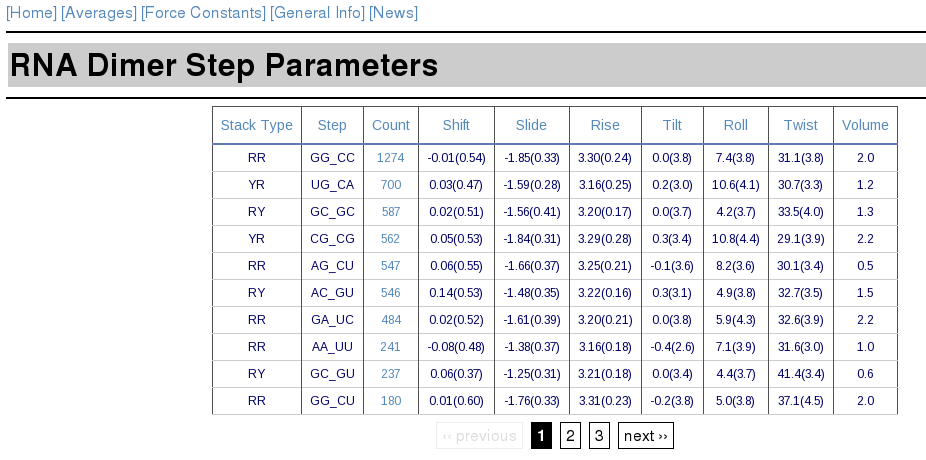
\includegraphics[angle=0, scale=0.4]{Chapter4/average.png}
\caption{Snapshot of the unique base-pair step parameters table for
  intact helical region RNA's, showing the fields that it can be
  sorted by. In this case it has been sorted by dimer step
  counts. There are three stack types purine-purine (RR),
  pyrimidine-purine (YR), and purine-pyrimidine (RY). The steps are
  denoted in a 5' to 3' sense, e.g., GG\_CC stands for a G$\cdot$C
  base-pair stacked on top of another G$\cdot$C pair with intact
  covalent linkage between G's, that is, GpG, and C's, i.e., CpG.}
\label{fig:average}
\end{figure}  

The values in  the table can be sorted by any  of the included fields,
that  is, Stack  Type, Step  Count,  Shift, Slide,  Rise, Tilt,  Roll,
Twist, Volume,  and RMSD. Also  the scatterplot corresponding  to each
step is  displayed when  clicking in the  counts column, along  with a
potential  energy contour  in  the  Roll-Twist plane  at  4.5 $kT$.  A
snapshot  of the  energy contour  for  the GG$\cdot$CC  step from  the
web-framework is shown in Figure ~\ref{fig:contour}.
\begin{figure}[htbp]
\centering
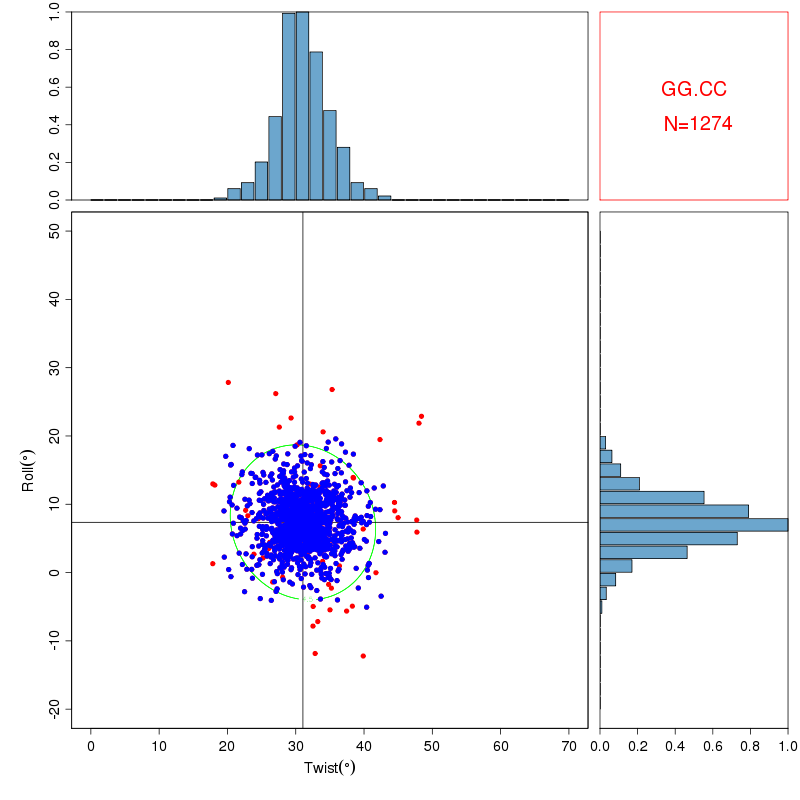
\includegraphics[angle=0, scale=0.4]{Chapter4/contour.png}
\caption{Snapshot from the web-framework of a scatterplot in the
  Roll-Twist plane with an energy contour. The full data before
  culling is show in red dots, and the culled data is shown as blue dots.} 
\label{fig:contour}
\end{figure}

The  other values  included  in  the web-framework  are  those of  the
force-constants corresponding  to the unique steps. A  snapshot of the
force-constant  matrix   for  the  GG$\cdot$CC  is   shown  in  Figure
~\ref{fig:forceconst}

\begin{figure}[htbp]
\centering
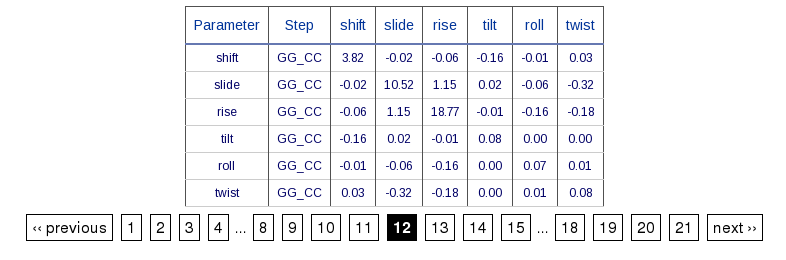
\includegraphics[angle=0, scale=0.6]{Chapter4/forceconst.png}
\caption{Figure showing a snapshot of the RNA Base-Pair Steps
  web-framework where the force constant matrix for the GG$\cdot$CC dimeric
  step is shown.}
\label{fig:forceconst}
\end{figure}  

\section{Persistence Length of RNA}
A quantity commonly used to  quantify the stiffness of polymers is the
so-called persistence  length $a$. To determine this  quantity for DNA
or RNA,  a variety of  theoretical and experimental techniques  can be
used.  Some  common experimental  techniques to determine  $a$ include
electron   microscopy   (EM),   gel   electrophoresis,   sedimentation
velocities, electrical birefringence,  atomic force microscopy (AFM) ,
magnetic  tweezers,  and small  angle  X-Ray  scattering (SAXS).   For
reviews  of  such  techniques  applied  to the  determination  of  RNA
persistence    length,    we   refer    the    reader   to    Hagerman
\cite{hagerman1997}, Abels  et al.  \cite{abels2005},  and Caliskan et
al.   \cite{caliskan2005}.  We  compare  our  simulation results,
based on  the "realistic" model  developed by Olson  and collaborators
\cite{olson1995} to describe DNA, with their findings. The "realistic"
model is dependent  on high-resolution crystallographic data.  Initial
studies started with small numbers  of data for the deformabilities of
the  ten unique  base-pair  steps \cite{olson1995}.   A more  complete
picture applied  to the study of DNA  sequence-dependent deformability
became  available   in  1998  \cite{olson1998}.    The  base-pair-step
deformability  data  for  DNA  has  been constantly  refined  as  more
high-resolution DNA and DNA-protein  structures have been added to the
Nucleic Acid Database (NDB) \cite{balasubramanian2009}.  Although such
data has been available for DNA  since 1998, such was not the case for
RNA, until recently \cite{olson2009}.

The  description of the  ``realistic'' model  along with  a simplified
schema of  the C++ code  developed by Luke  Czapla to implement  it, is
given  in Appendix~\ref{appendix4a}.  Also  in such  Appendix a  brief
account of  various definitions of  persistence length and  the models
generally used to compute it is given.

Using  the mean  values and  force  constants of  RNA base-pair  steps
available at our  web-framework we can use the  ``realistic'' model as
implemented  by  Czapla~\ref{czapla2006}  to compute  the  persistence
length  of chains  of increasing  lengths formed  from the  ten unique
base-pair  steps  of canonical  Watson-Crick  G$\cdot$C and  A$\cdot$U
pairs.   We  used two  rest  states  in  our calculations,  one  which
corresponds to  a naturally straight chain using  the standard dimeric
parameters for  the A-RNA conformation,  that is, $x_{i}^{0} =  \{0, 0,
  3.30,  0,  0,  31.6\}$ with   a  helical  repeat  of  11  base-pairs
\cite{arnott1999}.   The  other  rest  states  used  are  the  average
base-step   parameters   for    unique   steps   obtained   from   our
web-framework. It's  important to  note that one  cannot have  a chain
composed of  pure GC$\cdot$GC  steps, for example,  since the  step in
between two  such steps is  necessarily a CG$\cdot$CG  step, therefore
eight of the  ten chains formed by the unique  base-pair steps will be
mixed, and  only two will be made  purely from a single  kind of step,
that  is, those  chains formed  from the  GG$\cdot$CC  and AA$\cdot$UU
dimers.

As is expected the persistence lengths for naturally straight chains
are larger than the corresponding chains whose rest states are those
coming from the averaged crystallographic data as seen in
Figure~\ref{fig:perVlen}.

\begin{figure}
\centering
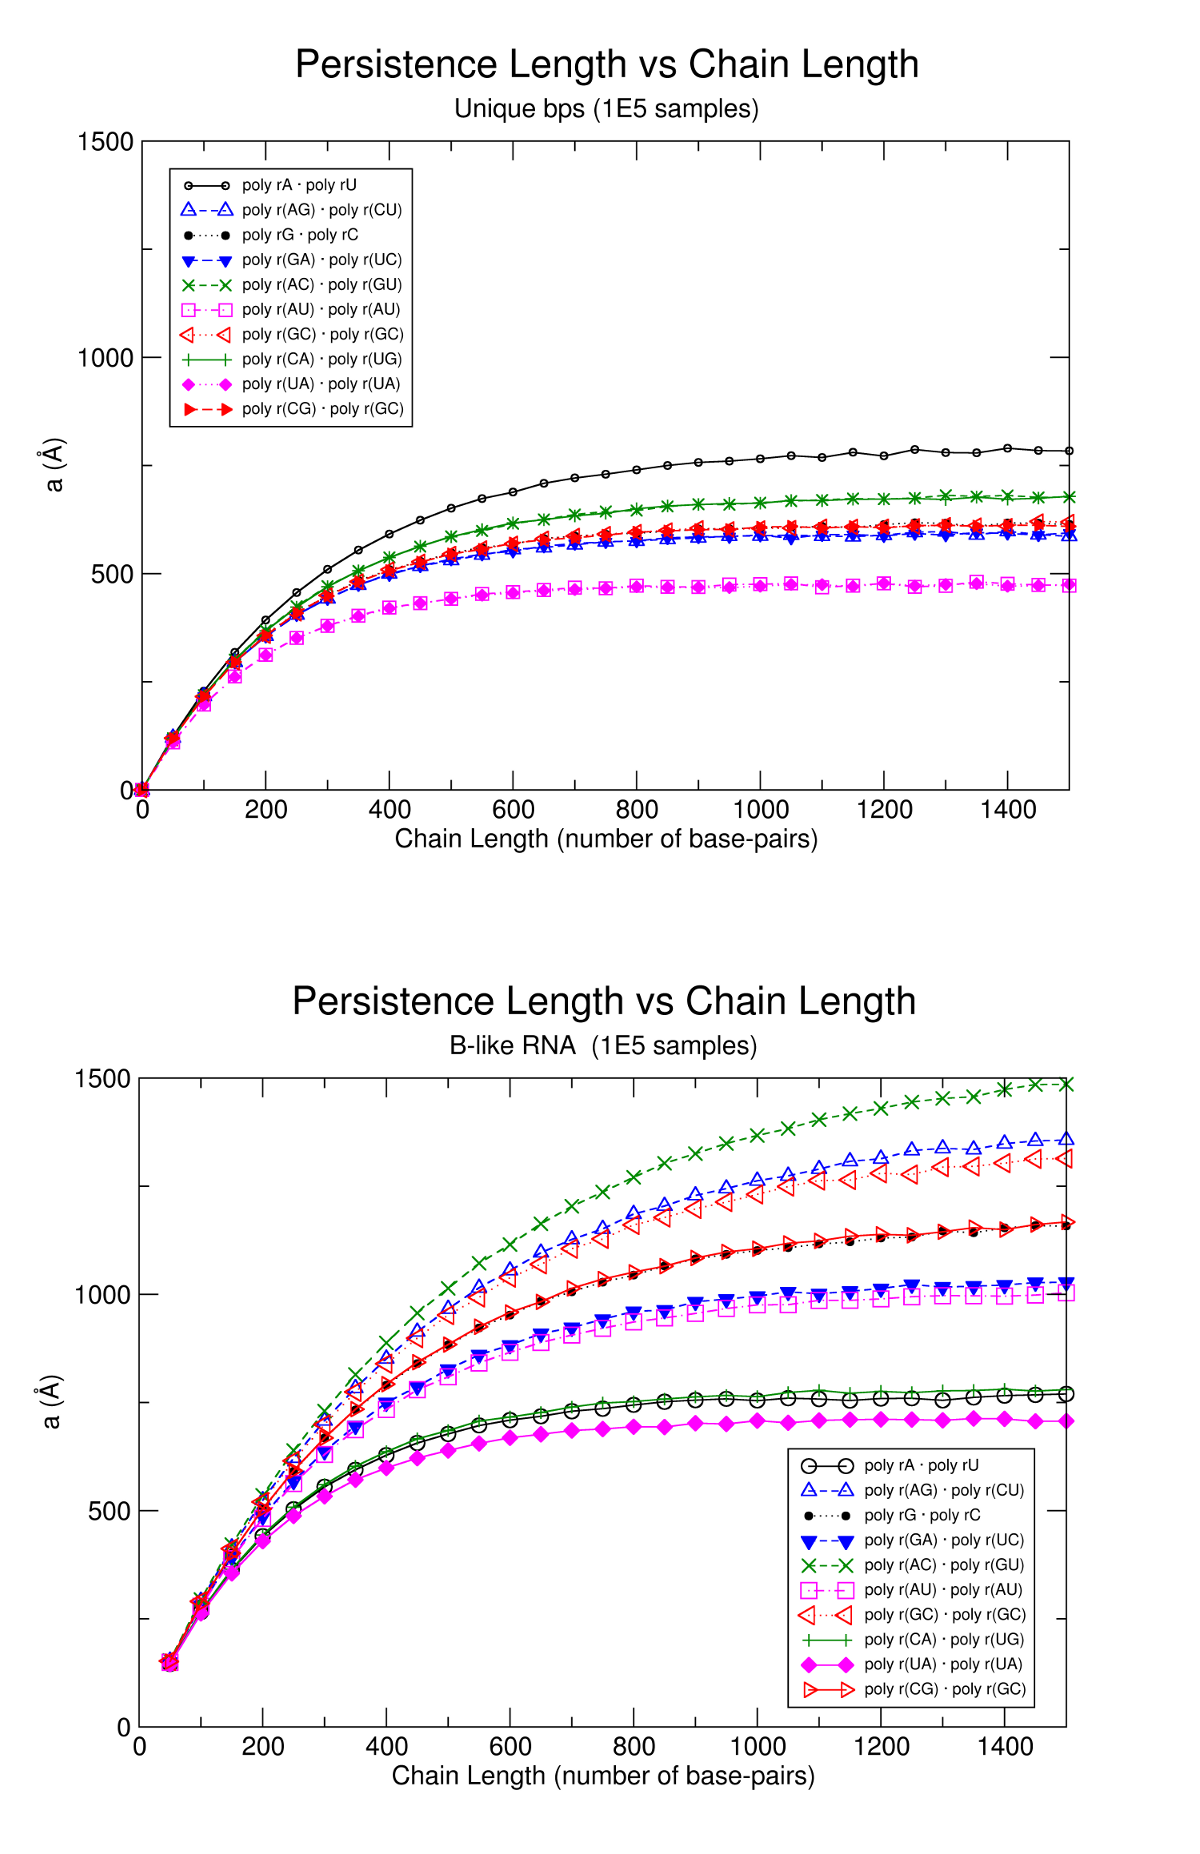
\includegraphics[angle=0, scale=2.8]{Chapter4/perVlen.png}
\caption{In the lower frame persistence length vs chain length in
  base-pairs for naturally straigth chains. In the upper frame the
  persistence length vs. chain length of ``real'' chains.}
\label{fig:perVlen}
\end{figure}


We also computed the persistence length at increasing chain lengths
for a mixed sequence RNA, where we see that a curved.

For comparison to the DNA case we computed the persistence length of a
1000 bp sequence with larger sampling for chains made up from the
unique dimers and using as rest state the values for a naturally
straight chain. We also constructed a random sequence with a
1:1 ratio of A$\cdot$U and G$\cdot$C which is compared to the
values obtained by Abels et al, and those of Hagerman in Table
\ref{tab:compare}. 




%\section{AMBER: Persistence Length of Base-Pair Step Patterns}
%I guess it needs some input here in order to work on latex compilation.



%CHAPTER OUTLINE

%- Methods Paper Results / Trends from counts
%  - Data culled.
%- Step Parameters. Conf Vols, RMSD
%- Equipotential Curves

%- Webserver
%  -table counts
%  -table force constants
%  -potential curves
%  -superimposed structures

%- Persistence Length RNA


% Technical pipeline details
%- Collection of base-pair steps data in helical regions.
%  - Yurong's bps database
%  - Yurong's python 3dnaparser
%  - scripts to change signs, assamble unique steps, and do stats.
%  - scripts to cull data
%  - scripts for deformation score
%  - reconstruction and RMSD calculation
%  - scripts for force-constant-matrices


\bibliography{biblio}


\chapter{RNA Motifs}
\label{motifs} 
\bibliographystyle{nar}
As mentioned  in Chapter 2,  until  now the most  common perspectives on
RNA motif recognition  and discovery have been chemical,  based on the
atoms  and bonds.  The  rigid-body based  perspective involved  in the
interactions and the internal parameters taht describe the 3D folds on
RNA motifs, by contrast, has  been rather unexplored.  In this chapter
we address two main questions:

\begin{enumerate}
\item{Can the  geometric, rigid-block description  of base-pairing and
  base-stacking help to define RNA structural motifs?}
\item{Can quantities derived from the 3DNA software package be used to
  perform an automated search for  known RNA motifs, such as, the GNRA
  tetraloop motif, and perhaps to find unknown RNA motifs?}
\end{enumerate}

We start with the second  question, testing the characteristics of the
base arrangements  in the  well known GNRA  tetraloop motif.   We have
also  examined  other   quantities  (e.g.   endocyclic  and  exocyclic
base-overlaps) obtained with 3DNA \cite{lu2003, lu2008b} to complement
the automated search for GNRA tetraloop motifs.

\section{The GNRA Tetraloop}
The GNRA motif  was initially found to be  an important constituent of
the small  subunit of the ribosome from  comparative sequence analyses
\cite{woese1990}. That  is, the GNRA sequence  was frequently repeated
among various organisms in tetraloop  regions of RNA, as were the CUUG
and UNCG  tetraloop sequences. These three sequences  account for more
than  70\% of  all tetraloops,  i.e.  single-stranded  loops  of four,
non-WC paired nucleotides,  found in the 16S subunit  of ribosomal RNA
\cite{woese1990, depaul2010}.  The most abundant of all the tetraloops
in the  ribosome is the GNRA  motif, and its  structural stability was
initially  characterized  using NMR  spectroscopy  by  Heus and  Pardi
\cite{heus1991}.   They   report  that  the   loop  is  closed   by  a
non-canonical sheared G$\cdot$A base-pair  and further stabilized by a
hydrogen  bond between  the  terminal guanine  base  and a  phosphate,
extensive  base stacking, and  a potential  hydrogen bond  between the
hydroxyl group in  the ribose at the 2$'$ end  of the terminal guanine
and the N7 of a  purine (R) base \cite{heus1991}. These features which
were later  confirmed in subsequent  X-ray structures \cite{pley1994b}
can be seen in Figure \ref{fig:gnrablocks}.

\begin{figure}
\centering
%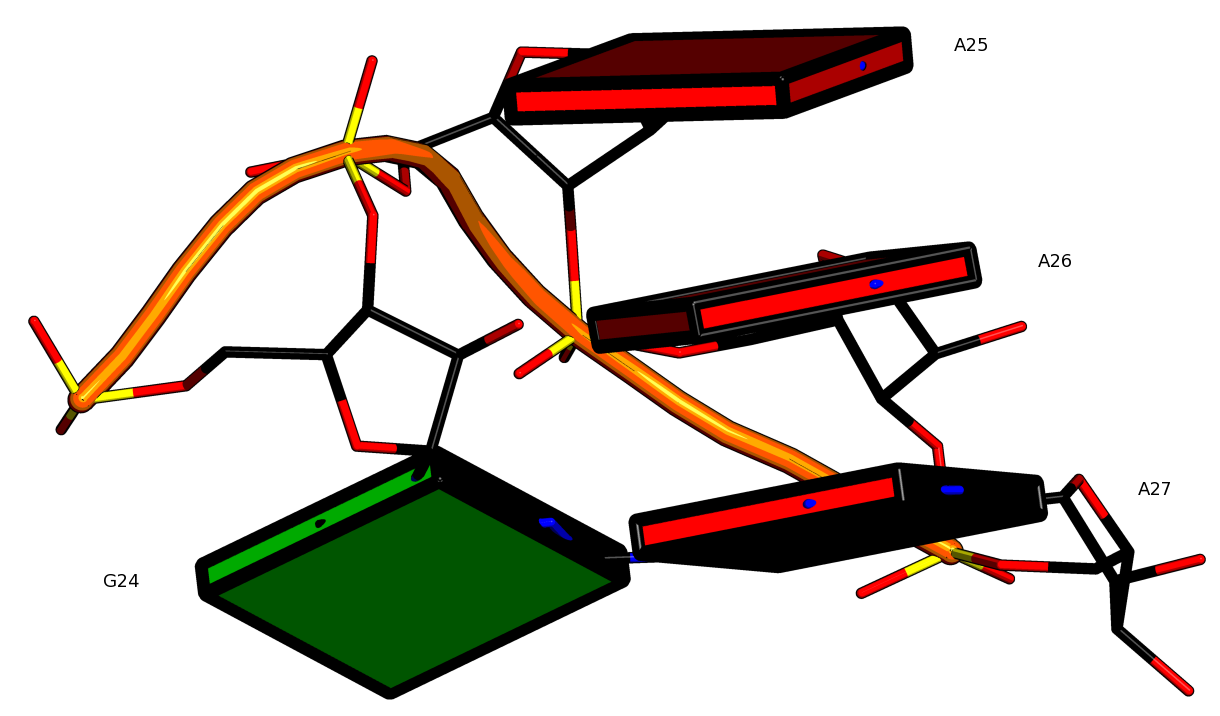
\includegraphics[angle=0]{Chapter5/gnra24.png}
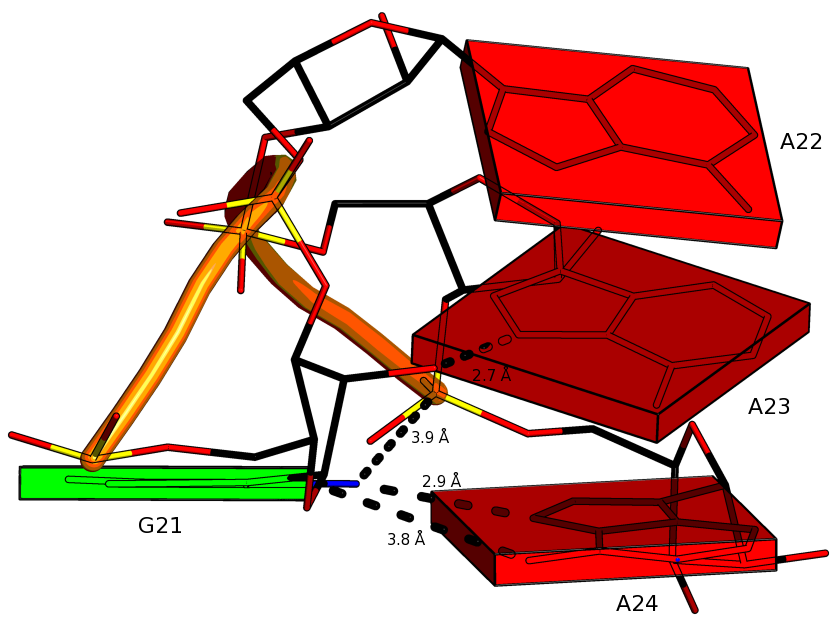
\includegraphics[angle=0, scale=0.38]{Chapter5/gnra21L2.png}
\caption{The   GNRA  tetraloop  motif   in  the   hammerhead  ribozyme
  PDB\_ID:1HMH \cite{pley1994}.  Although  not a newly recognized GNRA
  tetraloop, this motif is  positively recognized using our rigid-body
  parameters RNA motif search  program ``getMotif''. The structure was
  selected from a non-redundant list of RNA structures provided by the
  RNA  ontology consortium  (ROC)  \cite{leontis2006b}.  The  hydrogen
  bonding  interactions described  by Heus  and  Pardi \cite{heus1991}
  detected  in NMR  experiments are  shown  by black  and blue  dashed
  lines.}
\label{fig:gnrablocks}
\end{figure}

The description of  the GNRA tetraloop motif is a  typical case of the
problem  of RNA  motif definition.   For  example, in  the context  of
sequence  alone  a  GNRA motif  would  be  one  which contains,  in  a
consecutive  manner,  the  GNRA  pattern  of bases.   There  are  GNRA
structures, however,  which are not  formed by a  consecutive sequence
but  rather   have  the  same   geometric  arrangement  of   bases  in
three-dimensional  space   as  the  sequentially   linked  GNRA  motif
\cite{lee2003, lemieux2006}.  There are also structures which have the
same geometric arrangement and sugar-phosphate backbone connections as
the GNRA tetraloop,  but do not have the same sequence  of bases as in
the UCAA,  UCAC, CAGA, and CAAC  tetraloops \cite{lemieux2006}.  These
other  sequences  which  are  geometrically  equivalent  to  the  GNRA
tetraloop motif  form non-canonical base-pairs which  are isosteric to
the sheared  G$\cdot$A base-pair.  That is, the  U$\cdot$A, U$\cdot$C,
C$\cdot$A, and C$\cdot$C  base-pairs closing the respective tetraloops
are isosteric to  the G$\cdot$A base-pair at the end  of the GNRA loop
\cite{lemieux2006}.

A  number  of  molecular  dynamics  (MD)  studies  have  explored  the
conformational   space  of   the  GNRA   tetraloop  \cite{cornell1995,
  sorin2002, spackova2010,  depaul2010}. These  studies find a  set of
conformational states  for the GNRA tetraloop motif  which are closely
related  to existing X-Ray  and NMR  structures available  through the
Protein Data Bank \cite{depaul2010, sorin2002}.  Other MD studies have
used the well known GNRA  motif conformation as the starting point for
simulation  of other  tetraloops  \cite{srinivasan1998}.  These  other
tetraloops do  not retain  a GNRA-like three-dimensional  structure in
the simulations  \cite{srinivasan1998}, but this  effect might reflect
the force  fields used in such calculations  \cite{cornell1995} do not
correctly  predict  known  tetraloops  strucutures such  as  the  GAAA
tetraloop \cite{spackova2010}.

\subsection{GNRA Motif Search Program}
We have devised  a simple algorithm, ``getMotif'', to  search for GNRA
motifs  based  on  their  base  step  parameters.   The  algorithm  is
summarized in Figure \ref{fig:getMotif}.

\begin{figure}[ht]
\centering
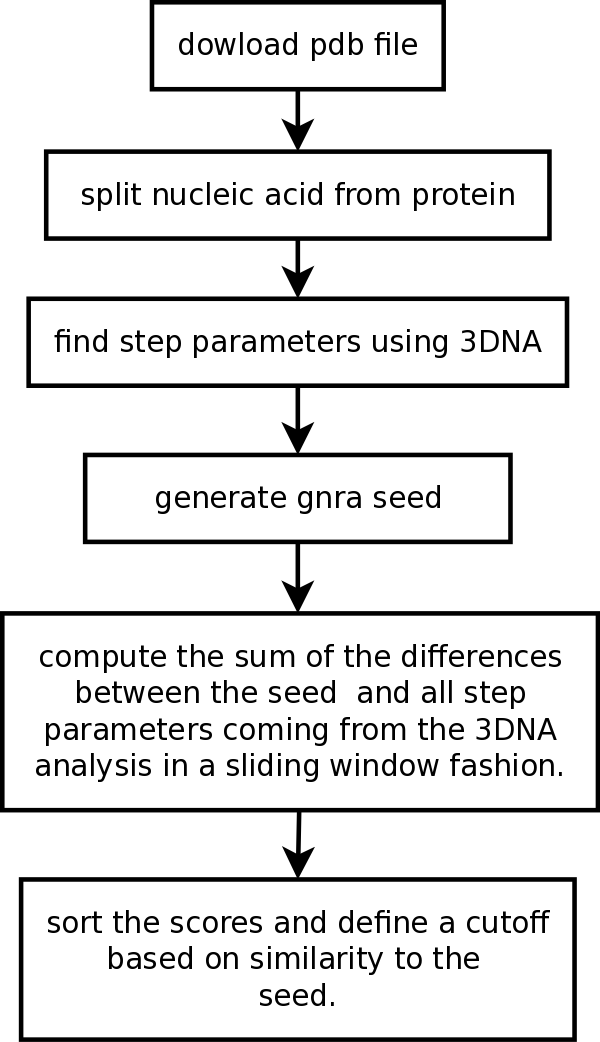
\includegraphics[angle=0, scale=0.4]{Chapter5/getMotif.png}
\caption{Simple algorithm  for GNRA motif  finding based on  base step
  parameters.}
\label{fig:getMotif}
\end{figure}
  
The algorithm allows for any motif  seed to be integrated into it, but
for now  we limit ourselves to  the use of  a seed formed by  the step
parameters  of  the GNRA  motifs  found in  the  23S  subunit of  rRNA
(PDB\_ID:1FFK)  by   Lemieux  et  al.    \cite{lemieux2006}.   We  are
currently  constructing a  database  of the  base-step parameters  for
known motifs,  so that our simple  program can be  expanded to include
various known  motifs that a user  wishes to localize  in an arbitrary
RNA structure or set of structures.

The  algorithm has  been programed  as a  simple, yet  very  fast bash
script \footnote{For  ease of use and  development a future  aim is to
  code the algorithm fully in python without compromising the speed of
  structure analysis.}  which interfaces  with three components -- one
written in  python, the  second being the  3DNA package, and  the last
written in the statistical analysis software \textbf{R}.  For example,
for the large subunit of the ribosome, PDB\_ID:1JJ2, the program takes
22.1 seconds to  download and analyze the whole  structure on an Intel
Core Duo of 2.13GHz with 8Gb of RAM.

The program  allows the user to  query any PDB\_ID. That  is, the user
only needs to  input in the command line of  a UNIX/LINUX terminal the
command, ``getMotif'' followed  by the PDB\_ID of the  RNA molecule of
interest.  As  a result  the user obtains  a list composed  of residue
numbers corresponding to the location of the start of the motif in the
structure,  and a  score which  stands  for how  close or  far a  four
nucleotide  sequential structure  is from  the GNRA  motif  seed.  The
advantage of  our program  over other Windows-based  motif recognition
software,  aside from  providing a  new analysis  based  on rigid-body
parameters,  is  that it  allows  for  easy  integration of  automated
scripts  for processing large  lists of  known PDB  structures without
user intervention for the analysis of every structure. For example, in
the  RNA ontology  consortium  (ROC)  meeting of  May  2009 a  reduced
dataset        of        RNA        structures        found        at:
\url{https://docs.google.com/Doc?id=dhrmkfmn_13ftpbjcgq}    was   made
available to participants with the  purpose of allowing them to search
for  RNA motifs  which would  later be  compared among  groups.  Using
Windows-based  softwares   like  FR3D  \cite{sarver2008}   it's  quite
difficult for  the user  to submit  a large job  composed of  many PDB
structures to a  queing system, or a cluster  computing server. Such a
task is made simple using getMotif.

To construct  the seed for  the GNRA motif  we extracted the  first 20
GNRA tetraloop motifs found by Lemieux and Major \cite{lemieux2006} in
the  large subunit  of the  ribosome (PDB\_ID:1FFK)  as  summarized in
Figure 3  of their results.  After computing  the base-step parameters
with 3DNA for  each of these motifs, we  arranged their average values
in a three by six matrix $S$  where each row corresponds to one of the
three steps in the tetraloop.   These average values are show in Table
\ref{tab:seed}.

\begin{table}[hb]  
\begin{center}
\begin{tabular}{|c|c|c|c|c|c|c|}
\hline
Step & Shift & Slide & Rise & Tilt & Roll & Twist \\
\hline
GN & -9.77 & -1.90 & -4.93 & 71.8 & 124.0 & -57.5 \\
NR & 2.74 & -0.11 & 3.04 & 11.5 & 6.0 & 50.6 \\
RA & 1.11 & -0.20 & 3.01 & 9.5 & 6.1 & 42.4 \\
\hline
\end{tabular}
\caption{GNRA motif  seed composed of the average  base step parameter
  values for 20 GNRA motifs found in the large subunit of the ribosome
  PDB\_ID:1FFK \cite{lemieux2006}.}
\label{tab:seed}
\end{center}
\end{table}

We  then  compute  a  score  to determine  the  distance  between  all
sequences formed by  three sequential steps in a  given RNA structure,
and the GNRA  motif seed. The score is simply the  sum of the elements
of the difference matrix $X_{k}$,  where the difference is between the
base-step parameters in the GNRA seed matrix $S$ and the corresponding
parameters  for  three sequential  steps  in  each  one of  the  $k-3$
sequential 3  x 6 matrices $W_{k}$,  where $k$ is the  total number of
steps in the RNA structure.

\begin{gather}
X_{k} = |S - W_{k}| \\
\text{score}_{k} = \sum X_{m,n} 
\end{gather}  

The scores  obtained from analysis  of the large ribosomal  subunit of
the  ribosome PDB\_ID:1FFK  can be  seen in  the histogram  displayed in
Figure \ref{fig:gnrahist}.

\begin{figure}
\centering 
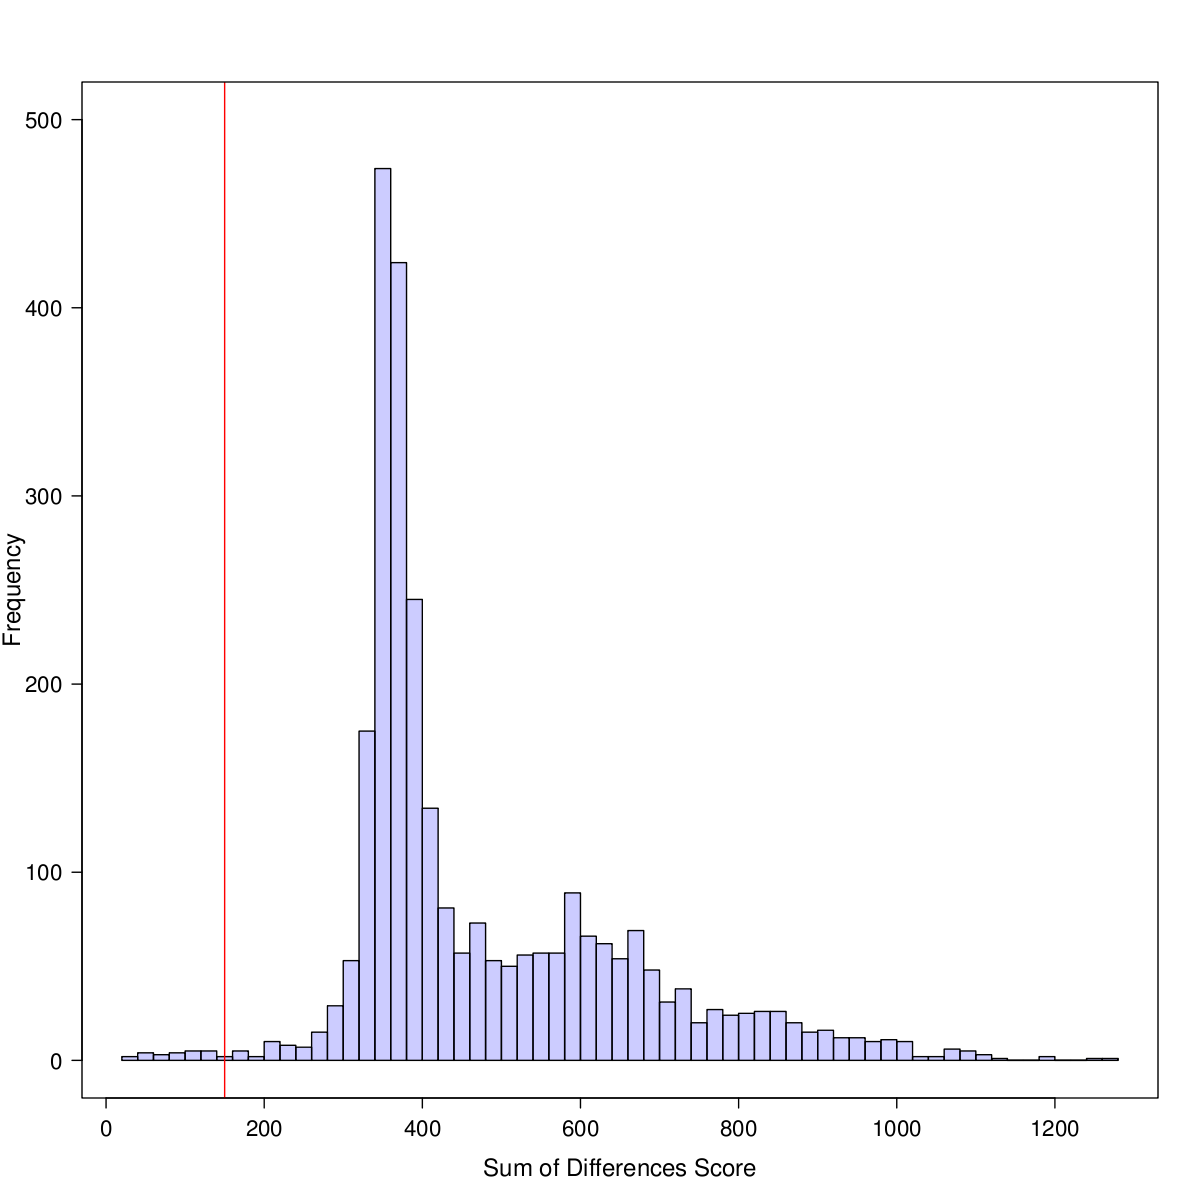
\includegraphics[angle=0, scale=0.5]{Chapter5/gnrahisto.png}
\caption{Histogram of  the sum of  differences score between  the GNRA
  seed  motif and  all  sequential tri-nucleotide-steps  found in  the
  large subunit of the ribosome PDB\_ID:1FFK}
\label{fig:gnrahist}
\end{figure}

In  this  histogram  we   see  that  the  majority  of  trinucleotides
(tristeps)  have scores  between  350-400.  These  values most  likely
correspond  to  tri-step  sequences  formed  by  base-step  parameters
similar to those of A-RNA-like  steps.  For our purposes of GNRA motif
identification we want to select those steps with scores which reflect
a shorter distance  to our seed GNRA motif.  Therefore  we have used a
cutoff score of 150, which is  represented by the values below the red
vertical line in Figure \ref{fig:gnrahist}.

Application of our program to  the list of 355 RNA structures provided
by the  ROC, with a  cutoff value of  150 finds \footnote{The  time it
  took  to search  for GNRA  tetraloop  motifs candidates  in the  355
  structures was 7  minutes and 29 seconds} 75  of these structures to
have at  least one GNRA  3D motif candidate,  and a total of  211 GNRA
motif  candidates.  The  list of  all  identified motifs  in these  75
structures including  the parameters at the first  step, are presented
in  Figure \ref{fig:steptype}  and  Table \ref{tab:gnrascores},  which
includes  an additional  check for  consistency  in the  next to  last
column.  The  latter entry  is the  overlap or the  ring atoms  of the
first two  bases of the tetraloop  which showed zero  in the described
structures.  Additionally the second  to last column shows the overlap
between  bases when  additional  exocyclic atoms  are considered,  for
example, the N4  amino atoms in cytosines \cite{lu2003}.   We see that
67\% of the identified GNRA motif candidates start with a GN step, and
interestingly that, almost one third  (27\%) of the first steps are UN
steps, and  that a few of the  identified motifs start with  AN and CN
dimers.

\begin{figure}
\centering
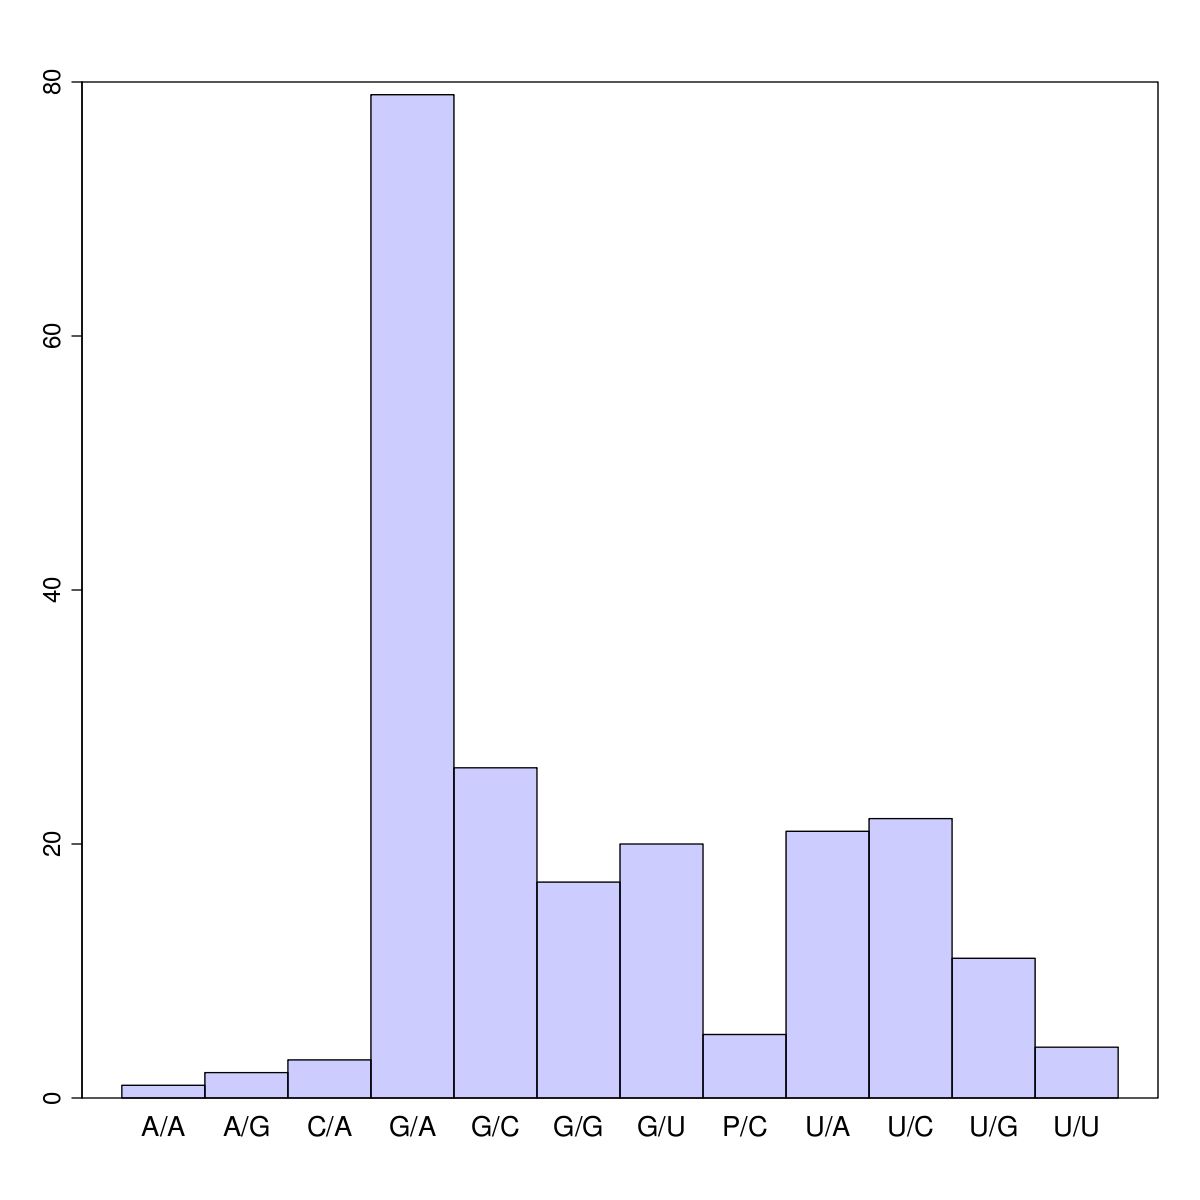
\includegraphics[angle=0, scale=0.5]{Chapter5/steptypesdist.png}
\caption{The barplot  above shows  the frequencies of  base-step types
  for the  first steps in  the candidate GNRA motifs  identified using
  ``getMotif''.  The  motifs have been  identified by similarity  to a
  base-step parameter seed constructed  from GNRA motifs found in the
  23S subunit of rRNA (PDB\_ID:1JJ2).}
\label{fig:steptype}
\end{figure}

To  further  analyze  the  results  of  the  motifs  identified  using
``getMotif'',  we   focused  attention  on   the  ribosomal  structure
(PDB\_ID:2J01) that  is included in the  ROC list.  As can  be seen in
Table   \ref{tab:gnrascores}  for  the   2J01  entries,   the  program
recognizes twenty  GNRA tetraloop motif  candidates, all of  which are
,in fact, tetraloops,  of these 13 conform to  the GNRA sequence, five
start with UN,  one starts with A  and one with C.  When  we align the
candidate GNRA motif sequences using  the reference frame of the first
two  bases,  we  see that  they  fall  into  two main  groups  (Figure
\ref{fig:groupsB}), one  with about eleven members and  the other with
seven members.  The  two remaining structures fit well  with the first
two steps, of both  groups I and II, but do not  fit well on the third
step in  either group.  Group  I, which is  colored in blue  in Figure
\ref{fig:groupsB} is closer to the  common GNRA motif. Group II, which
is  colored in  red  folds close  to  the common  GNRA  motif but  the
residues  which would  form  the terminal  G$\cdot$A  base-pair are  a
little  too   far  from  each   other  to  form  a   hydrogen  bonding
pattern. This variation stems from a  large rise in the last step. The
first two  steps are  very closely related  in every  case, suggesting
that there  is a subtle switch  between the tetraloop  and a pentaloop
conformation, governed by the rise in the last step.

\begin{figure}
\centering 
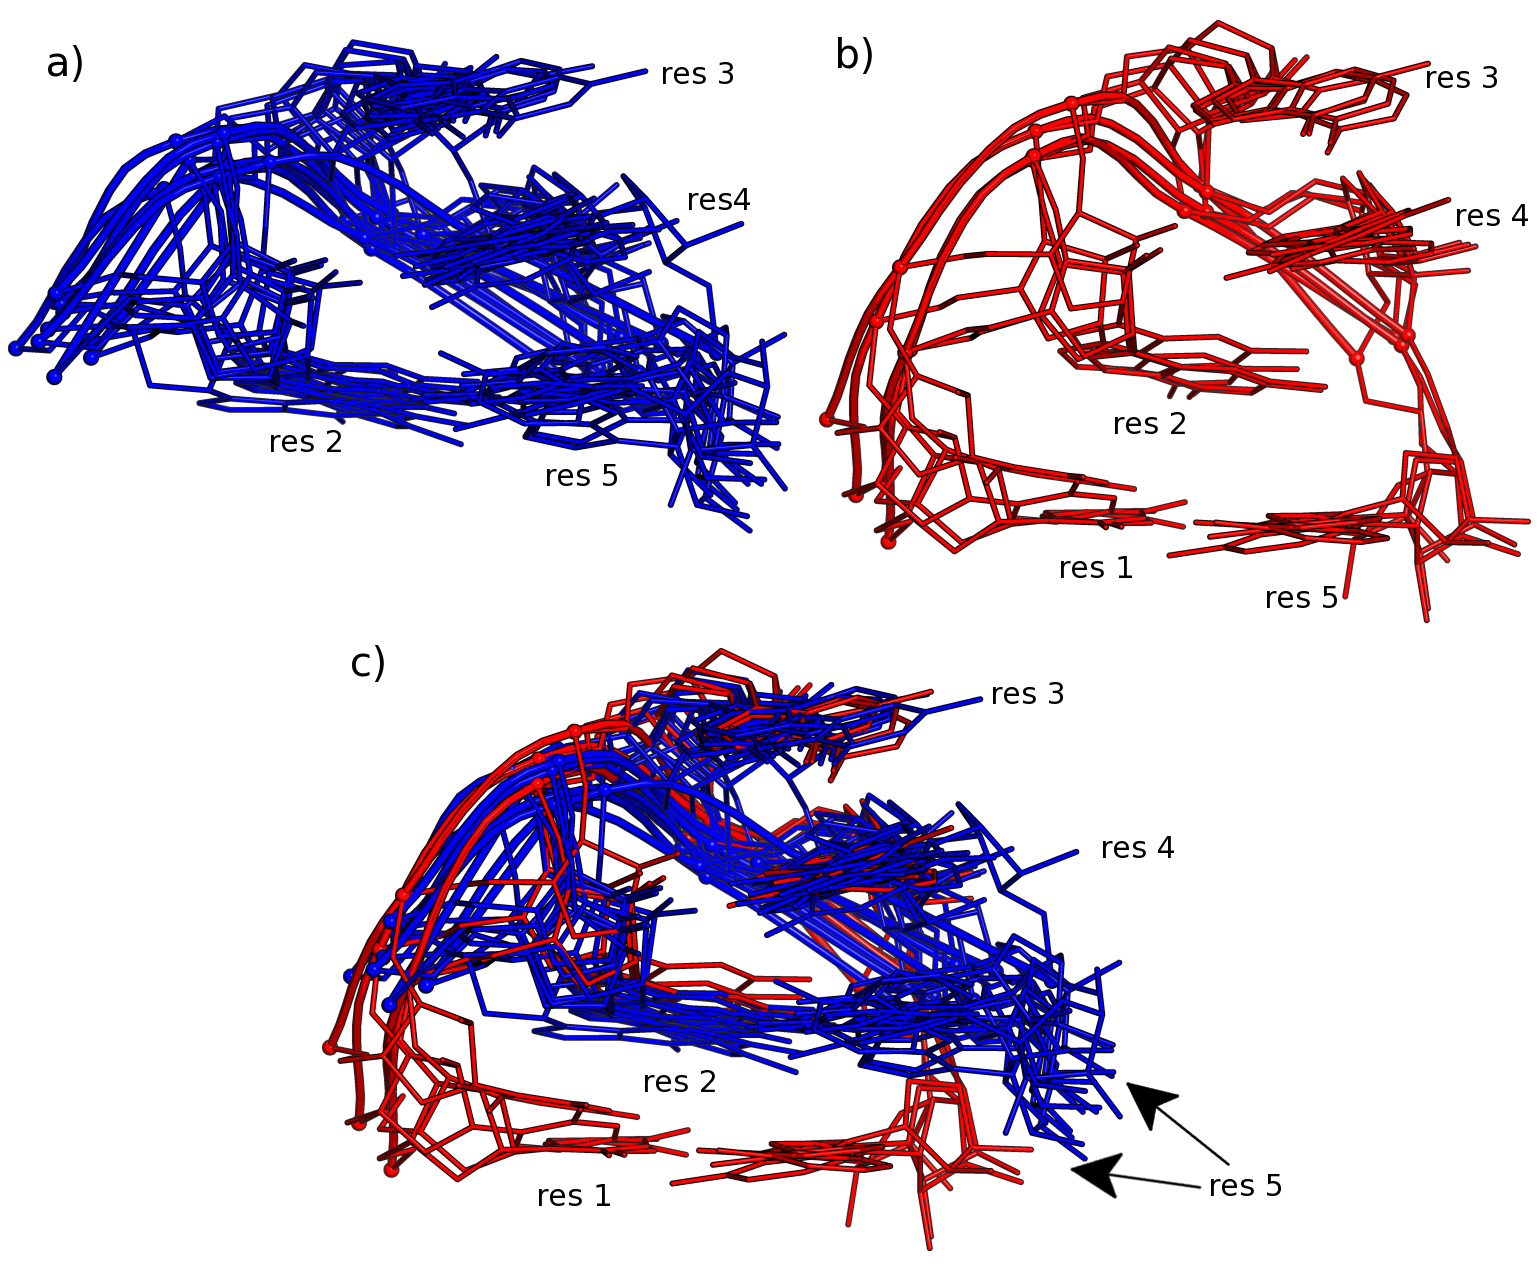
\includegraphics[angle=0, scale=2]{Chapter5/groupsB.png}
\caption{Two main groups of  tetranucleotide structures related to the
  GNRA  motif  identified  using  ``getMotif''.   All  structures  are
  superimposed  using  the  refence  frame between  residues  two  and
  three. In a)  Group I structures (RMSD []) which  are drawn in blue,
  are close  to a typical GNRA  motif.  The Group  II structures (RMSD
  [0.53-1.19])in b) which are drawn  in red are closer to a pentaloop.
  The steps  between residues  two and three,  and three and  four are
  common to the  two groups as is clearly  seen from the superposition
  of both groups  in c).  Residue two from Group  II is commonly found
  forming a  sheared G$\cdot$A  base-pair with a  sequentially distant
  base.   This type  of interaction,  which maintains  the  GNRA motif
  geometry and  is called a  lonepair triloop \cite{lee2003}  has been
  previously found from sequence covariation analyisis.}
\label{fig:groupsB}
\end{figure}

Interestingly some of  the GNRA candidates identified in  Group II are
part    of   a    highly   symmetrical    extended    "kissing"   loop
interaction. These  can be seen  in Figure \ref{fig:terts}  where they
are  superimposed, and  shown  in their  original  orientation in  the
ribosome. This type of interaction  is part of what has been described
as the lonepair triloop motif found by sequence covariation techniques
\cite{lee2003}.  The GNRA motif  candidates found by ``getMotif'' have
been named recently by Nasalean et al. \cite{nasalean2009} as internal
and composite motifs.  In our  case the GNRA motif candidates in Group
I  correspond to  the internal  motifs,  and the  Group II  candidates
correspond to the composite motifs of Nasalean and collaborators.

\begin{figure}
\centering 
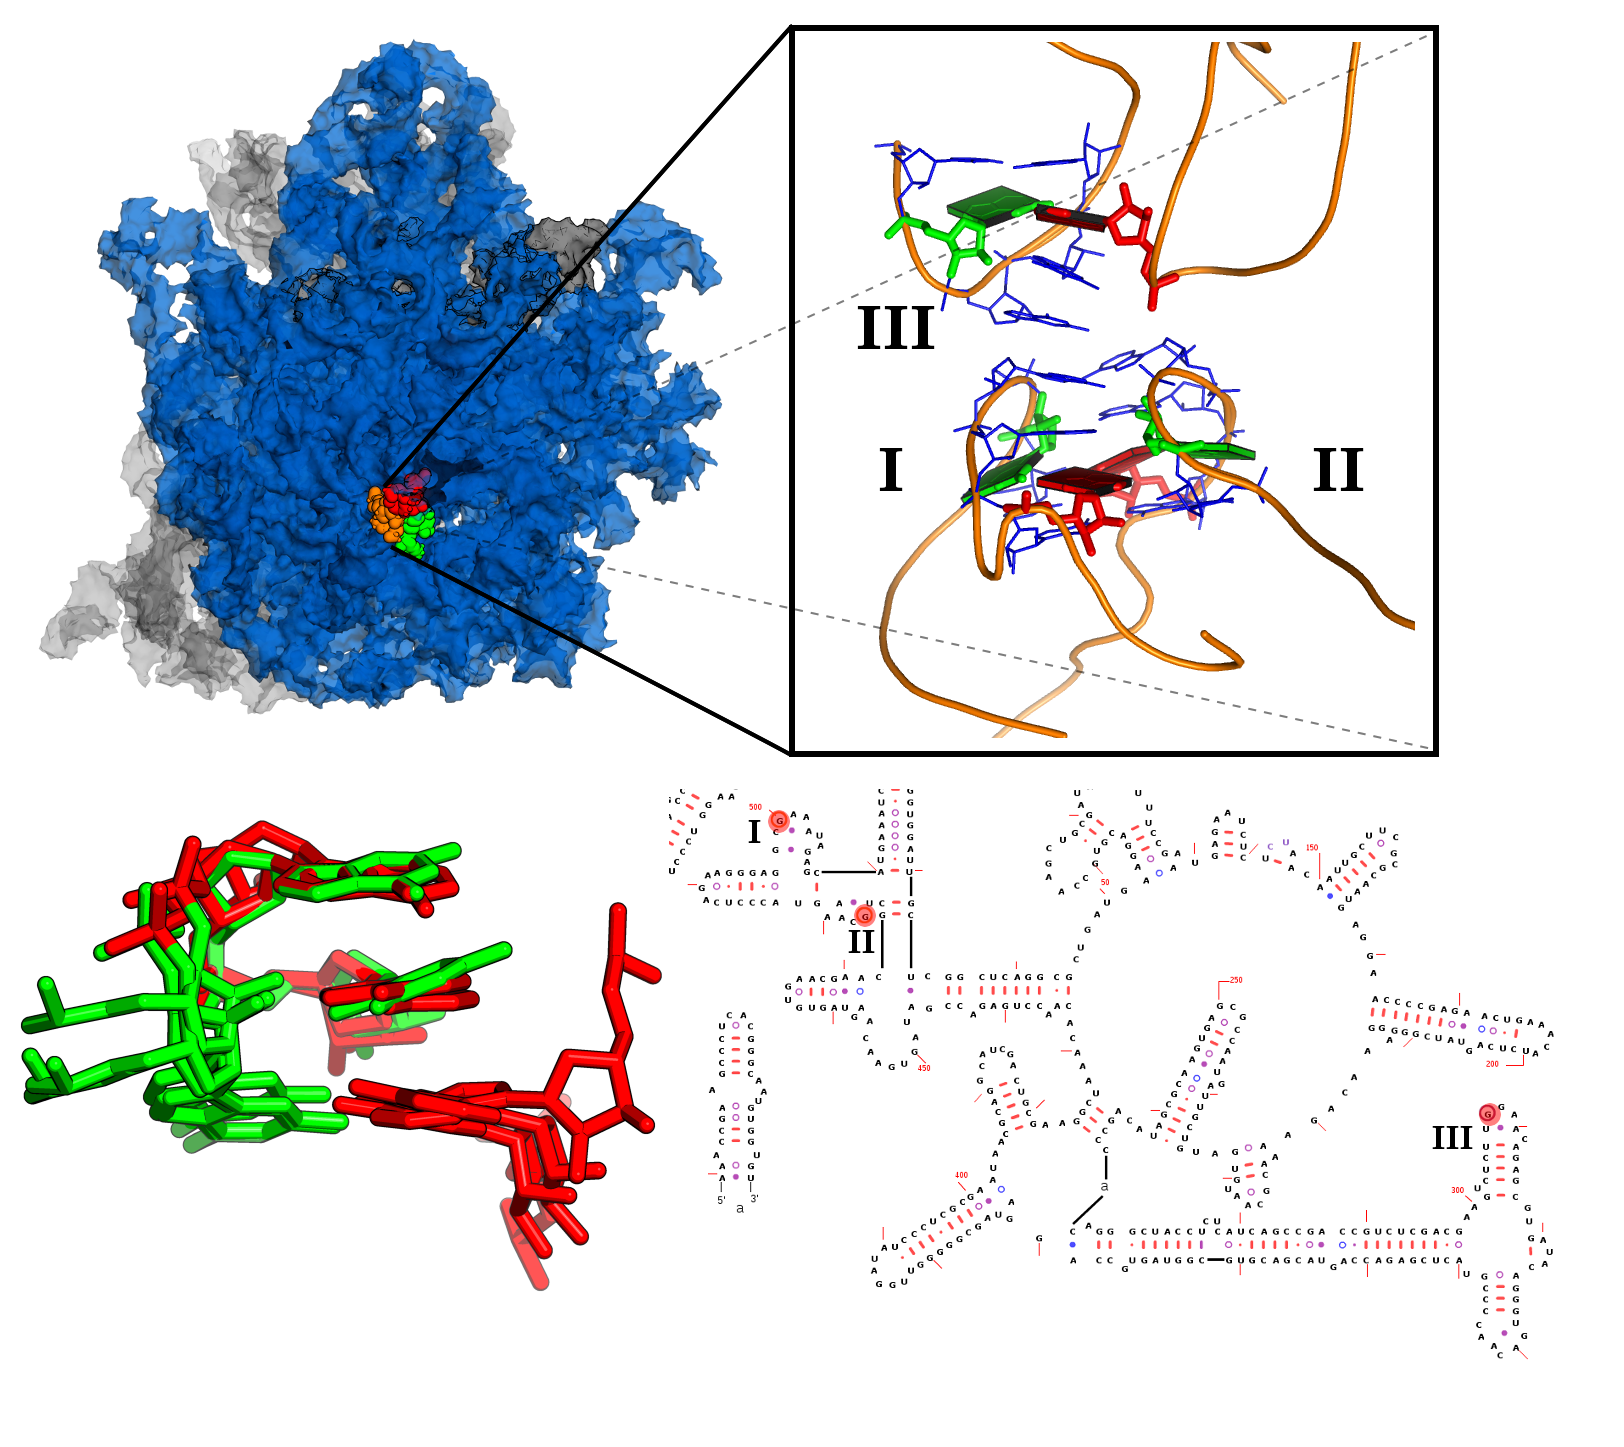
\includegraphics[angle=0, scale=0.34]{Chapter5/lonepairtlooptertF.png}
\caption{Subset   of   the  Group   II   structures  identified   with
  ``getMotif'',  which  correspond   to  the  lonepair  triloop  motif
  identified by Gutell and collaborators \cite{lee2003}.  In the upper
  left  corner of  the figure  sequentially distant  adenine  drawn in
  pink,  forms  a  sheared  G$\cdot$A base-pair  with  the  identified
  GroupII structure, which is drawn in red.  In the upper right corner
  of the figure the three  lonepair triloop motifs, or structural GNRA
  motifs are superimposed  in the reference frame of  residues two and
  three. In the lower portion of  the figure the location of the first
  residue of  the identified GNRA structural motifs  is highlighted in
  pink on top  of the secondary structure of the  large subunit of the
  ribosome, taken from Gutell Lab's website \cite{cannone2002}.  }
\label{fig:terts}
\end{figure}

Of the three steps which make  up the GNRA tetraloop, the first one is
the step farthest  away from a typical A-RNA-like  base-step.  We plot
the step-parameter  values for this  first step in the  scatterplot in
Figure \ref{fig:scattergnra}.  It is clear from  this scatterplot that
these  steps  constitute  a  well  defined  region  in  the  space  of
rigid-body step parameter configurations  for the large subunit of the
ribosome.

\begin{figure}
\centering 
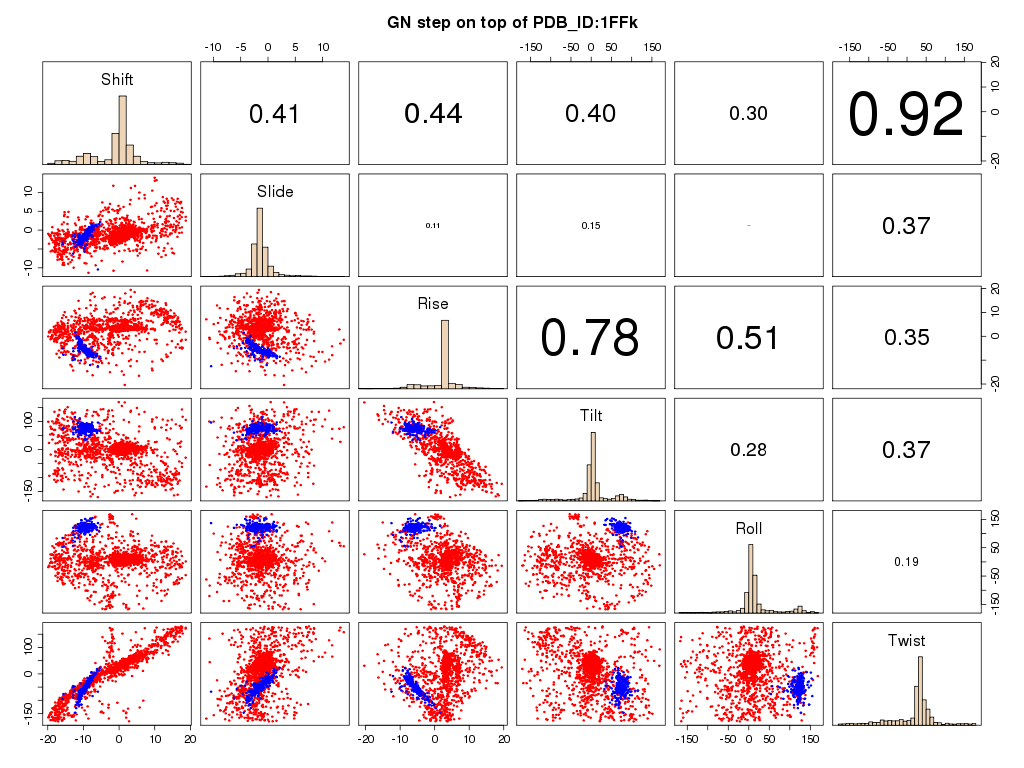
\includegraphics[angle=90, scale=0.5]{Chapter5/GNRAin1ffk.png}
\caption{Scatterplot  of  base-step parameter  values  for GNRA  motif
  candidates identified in a list given by the ROC, against a backdrop
  of the range of values  for the step-parameters in the large subunit
  of the ribosome PDB\_ID:1FFK.}
\label{fig:scattergnra}
\end{figure}

%\section{Canonical "Noise"}
%To be able to say anything about motifs it's crucial to get rid of the
%"noise" which is given by the canonical base-pair steps.
%One would think that perhaps  the X3DNA-Parser of Dr. Yurong Xin could
%help  in the  task, but  then, it  can't, because  it's based  on what
%base-pairs  have  been found,  therefore,  it  tells  me about  single
%stranded interactions,  it doesn't tell  me about bases which  are not
%forming interactions and are alone.

%\subsection{3DNA-Parser}
%We started by using Dr. Yurong Xin's 3DNA-Parser hoping that the
%description of the enclosing base pair in the loop, that is, the
%sheared G$\cdot$A, would have a characteristic signature.
%We found that such is not the case. We know from Major et
%al. \cite{lemieux2006} that there should be at least 21 GNRA tetraloops
%in the 23S subunit of rRNA. We used the G2696 N2697 R2698 A2699
%tetraloop as a seed (as can be seen in Figure 1.1) and found out
%that according to Dr. Xin's helical classification the enclosing G is
%classified as $S_{hq}$ and A is classified as $H_{e}$. 

%We then searched all such instances for G$\cdot$A base-pairs and we
%found seven hits, but none were in fact GNRA tetraloops.

%\subsection{Overlap Scores} 
%We  clustered the  overlap  values  impossing a  cutoff  of values  of
%[1-8]. Since a large amount of overlap values are exactly zero (33\%),
%so, without the cutoff the zero values "overshadow" the data.
%\begin{figure}[htbp]
%\centering 
%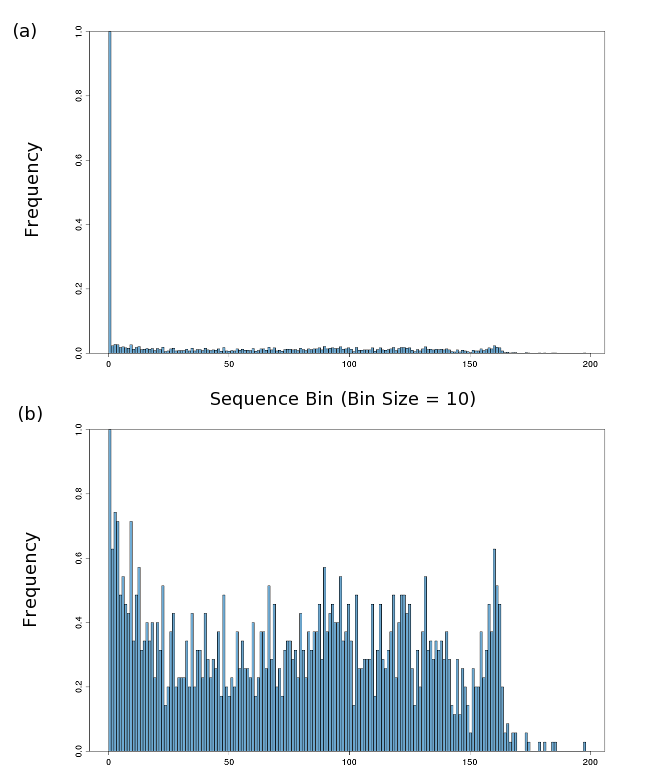
\includegraphics[angle=0, scale=0.8]{Chapter5/histocompare.png}
%\caption{Normalized  histograms showing  the  distribution of  overlap
%  values  in the  23S subunit  or \textit{Thermus  Thermophilus} rRNA,
%  PDB-ID:1jjk.  In  histogram (a)  all  values  are  included, but  in
%  histogram (b) only values greater than zero are included. Notice the
%  high preponderance  of zero  values, exactly 897  out of a  total of
%  2705.}
%\end{figure}
%For this case we obtain the dendrogram shown in Figure 1.2.
%\begin{figure}[htbp]
%\centering 
%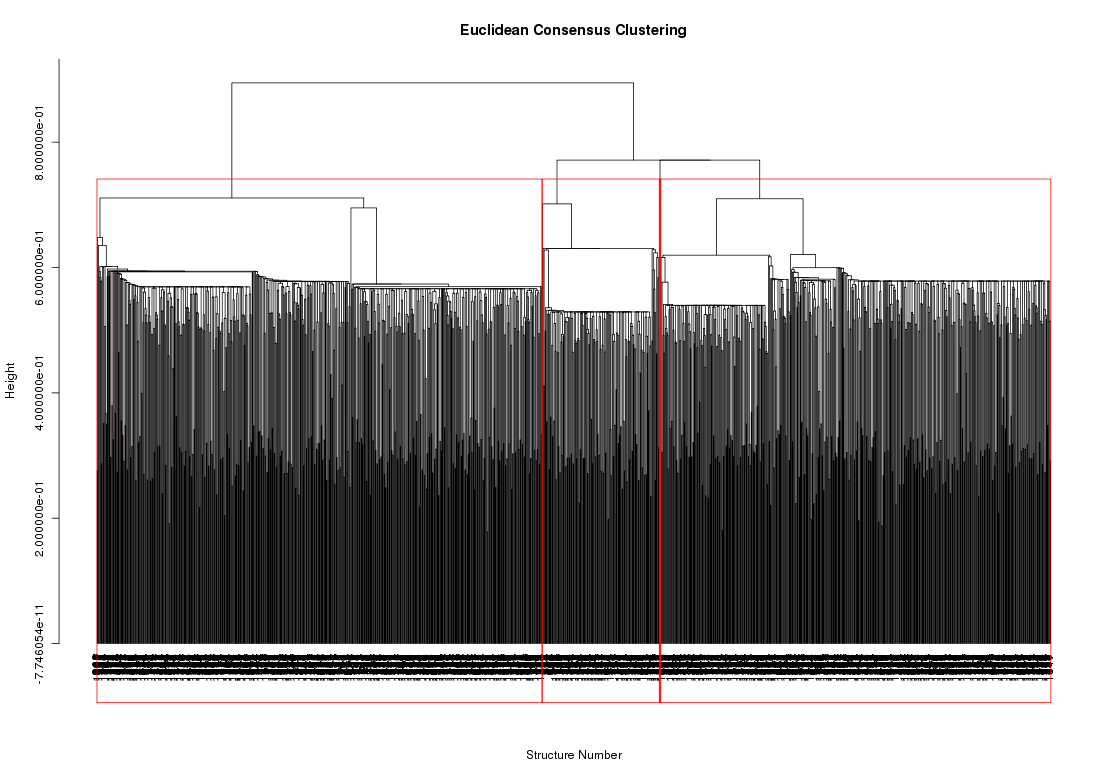
\includegraphics[angle=90, scale=0.6]{Chapter5/eucli_cons.png}
%\caption{Dendrogram for consensus clustering  of overlap scores in the
%  ribosome.  Zero values filtered out and remaining data normalized.}
%\end{figure}

%The next  step in this analysis  will be to find  the structures which
%correspond  to this  clusters  and superimpose  and  align them  using
%Kabsh's algorithm to be able to determine their RMSD's.

%Many people  start their  RNA Motif identification  and classification
%algorithms by splitting  RNA structures into what is  helical and what
%is not,  and then  finding interactions between  these two  groups. We
%believe that  we could do  a similar exercise  with 3DNA by  using the
%scalar  product   of  helical  axis  vectors  and   once  helical  and
%non-helical regions are  found we might be able to  use 3DNA Parser to
%look for characteristic interactions.

%\section{Triplets on RNA (comparison to Laing et al.)}

\section{Results on RNA Motif Recognition via Step-Parameters}

We previously asked ourselves if the geometric rigid-block description
of  base-pairing and  base-stacking could  help define  RNA structural
motifs.

We  believe that  the problem  of  defining RNA  structural motifs  is
clearly more complicated than what can be understood by any structural
research  methodology  alone,  such  as  those based  on  analysis  of
backbone  torsions,  or all-atom  fitting.   We  have  shown that  the
rigid-body  parameters  relating  sequential  bases  facilitate  motif
searches  in  RNA  atomic  structures  as  well  as  in  the  rigorous
description of structural  motifs. It has also been  shown in previous
work  on  RNA  in   the  Olson  group  \cite{yurongthesis},  that  the
rigid-body parameters  describing RNA base-pairs can help  to find and
describe novel  RNA tertiary interactions  important for understanding
the three-dimensional fold of the ribosome, for example, the role that
the  noncanonical sugar-edge  sugar-edge parallel  G$\cdot$A base-pair
plays as linker of sequentially  distant regions in the 50S subunit of
the  ribosome (PDB\_ID:1JJ2), and  it's relation  to known  RNA motifs
such  as  the   kink-turn  motif.  We  consider  that   this  type  of
characterizations and  their automation  with simple programs  such as
``getMotif''  should  prove  useful  to the  community  interested  in
ontological characterization of RNA.

Yet another specific question we  formulated inquires if we can use
quantities  derived  from  the  3DNA  software  package  to  make  and
automatic search  for a known  motif, for example, the  GNRA tetraloop
motif, and perhaps find unknown motifs?

We have found that by defining seeds from known motifs we can find new
motifs at the boundaries of  these ones through their base-steps.  For
example, we  started a GNRA  motif search using its  average base-step
parameters  from the  GNRA's found  in the  23S ribosomal  subunit and
found a closely related motif which  we have called Group II motif and
which in turn is part of a composite motif \cite{nasalean2009} that is
known as the lonepair triloop motif \cite{lee2003}.

We can also  perform other, simpler, but not  as ``precise'' RNA motif
searches,   e.g.  by   following  the   proposed   cluster  validation
methodology used in Chapter 2 to find an optimal method for clustering
other  3DNA-computed  properties of  smaller  dimensionality than  the
base-step parameters, for example, sequential base overlaps.

Searches of other rigid-body  parameters which have not been explored,
could also  be useful (such as the  helical parameters x-displacement,
y-displacement, inclination and tip relating sequential base steps).

\bibliography{biblio}


%\chapter{Introduction}
\label{introduction} 
\bibliographystyle{nar}
This is the introductory chapter.


\bibliography{biblio}


\appendix
\chapter{Standard reference frame and local parameters}
\label{appendix_1a}
\bibliographystyle{nar}  In   addition  to  the   description  of  RNA
structures  at the  level of  torsion  angles, one  can also  describe
structure  in  terms  of  the  spatial  arrangements  of  adjacent  or
associated bases.  The structural description  of RNA used  here comes
from the program \textsf{3DNA} \cite{lu2003}, which reports three sets
of parameters that define the local arrangements of bases.
\begin{enumerate}
\item Base-pair parameters,
\item Base (base-pair) step parameters,
\item Base (base-pair) local helical parameters.
\end{enumerate}
The base or  base-pairs parameters are the quantities  that bring into
coincidence  coordinate  frames  on   two  objects  using  ideas  from
classical mechanics.
%% The first two are based on cartesian coordinates
%% (``objectcentered'', reference frame),
%% whereas the third is referred as helical coordinates
%% (non-object centered)
The first two sets of parameters are based on Cartesian coordinates of
two base or  base-pairs, whereas the third set  of helical parameters,
resembles cylindrical coordinates and are based on the single rotation
that  brings  coordinate  frames  on  two  bases  or  base-pairs  into
coincidence (Chasles's theorem) \cite{babcock1994}.

\section{Base-pair and base-step parameters}
In \textsf{3DNA} one  starts with a Protein Data  Bank (PDB) formatted
\cite{berman2000}  file,  which   is  usually  based  on  experimental
information\footnote{A PDB file is sometimes the result of theoretical
  modeling.}   and  which can  be  downloaded  from  the Nucleic  Acid
Database (NDB)  or PDB.  This file contains  the Cartesian coordinates
and other  information, such as sequence composition,  about the given
structure of  the atoms.  With  this experimental data one  performs a
least-squares fit to a  standard reference frame \cite{olson2001}. The
\textsf{octave}                        script                       at
\url{http://www.eden.rutgers.edu/~esguerra/RNA/scripts.html}   provides
a useful tutorial example.  The coordinate origin which is embedded in
the standard  reference frame, is  used for the determination  of both
base and base-pair parameters.  In  the case of single unpaired bases,
the  program keeps the  origin of  one base  of an  ideal Watson-Crick
pair.    The   definition   of    this   frame   is   illustrated   in
Figure~\ref{fig:standard}

\begin{figure}[htbp]
\centering
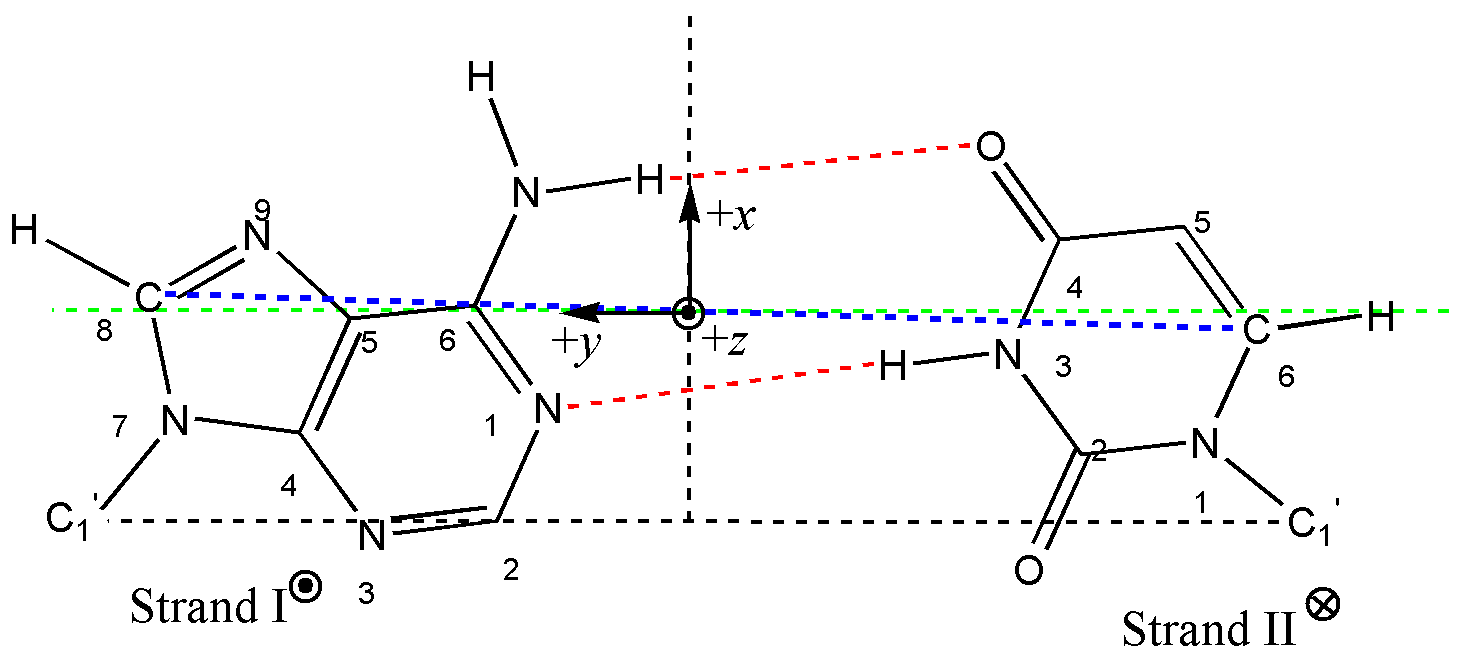
\includegraphics[scale=0.8]{Chapter1/standard.png}
\caption{Standard    reference    frame    of   an    A-T    base-pair
  \cite{olson2001}.  The \textit{y}-axis (dashed green line) is chosen
  to be  parallel to the line  connecting the C1$^{'}$  of adenine and
  the  C1$^{'}$  of  thymine   associated  in  an  ideal  Watson-Crick
  base-pair. The \textit{x}-axis is  the perpendicular bisector of the
  C1$^{'}$  -  C1$^{'}$  line,  and  the  origin  is  located  at  the
  intersection of  the \textit{x}-axis and the line  connecting the C8
  atom of adenine  and the C6 atom of  thymine. The \textit{z}-axis is
  normal  to the  base-pair plane  (defined in  a positive  sense with
  respect to the leading base, here A) and the direction of the x-axis
  is defined by the cross  product of the $\hat{x}$ and $\hat{y}$ unit
  vectors.}
\label{fig:standard}
\end{figure}

After the  coordinate origins for  two consecutive base  of base-pairs
comprising a  step have  been computed, then  a so-called  middle step
triad (MST)  \cite{lu1997} is defined. Defining the  middle step triad
is described by the following procedure:

1) Find the angle $\Gamma$ between consecutive normals, \textit{i.e.},
\textit{z}-axes. Since these are unit vectors, the angle is defined by
the scalar product:

\begin{gather}
\Gamma = \cos^{-1} (\hat{z}_i \cdot \hat{z}_{i+1})
\end{gather}

2)  Then find the  vector which  is perpendicular  to the  two normals
(\textit{z}-axis). This  vector is obtained from the  cross product of
the  consecutive \textit{z}-axes  (that is,  the normal  to  the plane
formed by the two vectors). This axis is called the roll-tilt axis and
is normalized to form the unit vector $\hat{r_t}$,

\begin{gather}
\hat{r_t} = \frac{\hat{z}_i \times \hat{z}_{i+1}}{|\hat{z}_i \times
\hat{z}_{i+1}|}
\end{gather}

%% Note: Why do you need a matrix? Isn't this always in 3D and therefore
%% just vectors would do? Why the more general matricial way instead of
%% the vectorial representation?
3) To make consecutive \textit{z}  vectors coincide, one uses a linear
homogeneous transformation  $R(\theta)$ about the  roll-tilt axis such
that the  original orientation matrices $T_i$ and  $T_{i+1}$, i.e. the
set  of unit  vectors  along  the x,  y  and z-axes  of  each base  or
base-pair specified in the columns of  each, are rotated by $ \theta =
\pm \Gamma /  2$ to yield the transformed  $T_i^{'}$ and $T_{i+1}^{'}$
orientation matrices.
%% NEED to include GRAPHICS of ANGLES and COORDINATES in general.

\begin{gather}
T_i^{'} = R_{rt}(\pm \Gamma/2) T_{i} \\
T_{i+1}^{'} = R_{rt}(\mp \Gamma/2) T_{i+1}
\end{gather}

The origin  for the middle step  triad (MST) is the average  of the position
vectors $r_{i}$ and $r_{i+1}$ for the $i$ and $i+1$ reference frames,

\begin{gather}
r_{MST} = \frac{(r_i + r_{i+1})} {2}
\end{gather}

4) Again  using the  dot product  one can find  the angle  between the
transformed  $\hat{y}^{'}$  vectors.   This  angle  is  equal  to  the
magnitude of the Twist ($\Omega$)  in the base of consecutive bases or
base-pairs.  The  dot product  of the $z$  unit vector for  the middle
step triad  (MST) $\hat{z}_{MST}$ with  the vector resulting  from the
cross product  of $\hat{y}_{i}^{'}$ and  $\hat{y}_{i+1}^{'}$ gives the
sign  of  $\Omega$.  Since   the  transformed  \textit{x-y}  plane  is
orthogonal  to $\hat{z}$  then this  applies  in the  same manner  for
\textit{x},  %%The vector  resulting from  (yi X  yi+1 has  got  to be
parallel or %%anti-parallel to zMST, there's no other possibility.

\begin{gather}
\Omega = cos^{-1}(\hat{y}_{i}^{'} \cdot \hat{y}_{i+1}^{'})\\
(\hat{y}_{i}^{'} \times \hat{y}_{i+1}^{'}) \cdot \hat{z}_{MST} > 0, \quad \textrm{then} \ \Omega > 0\\
(\hat{y}_{i}^{'} \times \hat{y}_{i+1}^{'}) \cdot \hat{z}_{MST} < 0, \quad \textrm{then} \ \Omega < 0
\end{gather}

%%if normalized beforehand then the rule would be,
%%\begin{gather}
%%(\hat{y}_{i}^{'} \times \hat{y}_{i+1}^{'}) \cdot \hat{z}_{mst} = 1, \quad %%then \ \Omega > 1\\
%%(\hat{y}_{i}^{'} \times \hat{y}_{i+1}^{'}) \cdot \hat{z}_{mst} =
%%-1,\quad then \ \Omega < -1
%%\end{gather}

5) With more scalar product one  can find other angles, such as the phase
angle $\phi$,
%% Show in figure.

\begin{gather}
\phi = cos^{-1}(\hat{rt} \cdot \hat{y}_{MST})\\
(\hat{rt} \times \hat{y}_{MST}) \cdot \hat{z}_{MST} > 0, \quad \textrm{then} \ 180 \geq \phi \geq 0\\
(\hat{rt} \times \hat{y}_{MST}) \cdot \hat{z}_{MST} < 0, \quad \textrm{then} \ -180 \leq \phi \leq 0
\end{gather}

6) The  roll $\rho$  and tilt $\tau$  angles, which are  the remaining
angular degrees of  freedom for step parameters, are  defined in terms
of the bending angle and the phase angle:
%as if we were doing a change of variables from cartesian to polar.

\begin{gather}
\rho = \Gamma cos (\phi)\\
\tau = \Gamma sin (\phi)
\end{gather}

To  get the remaining  three translational degrees of  freedom for
step  parameters  ($Dx,  Dy,  Dz$)  one  needs  to  express  the
displacement vector in the middle step triad frame:

\begin{gather}
[D_xD_yD_z]=T_{MST}(r_{i+1} - r_{i})
\end{gather}

The  procedure  to  compute  the base-pair  parameters  is  completely
analogous.   The  opening  $\omega$,  buckle $\kappa$,  and  propeller
$\sigma$  are the  analogs of  twist $\Omega$,  roll $\rho$,  and tilt
$\tau$, and the middle step triad is called the middle base triad MBT.
The axes  which are made to  coincide are the  \textit{y}-axes and not
the \textit{z}-axes as in the base-pair step case \cite{lu1997}.

The parameters obtained by  this procedure are depicted graphically in
Figure~\ref{fig:allparam}.
\begin{figure}[htbp]
\centering
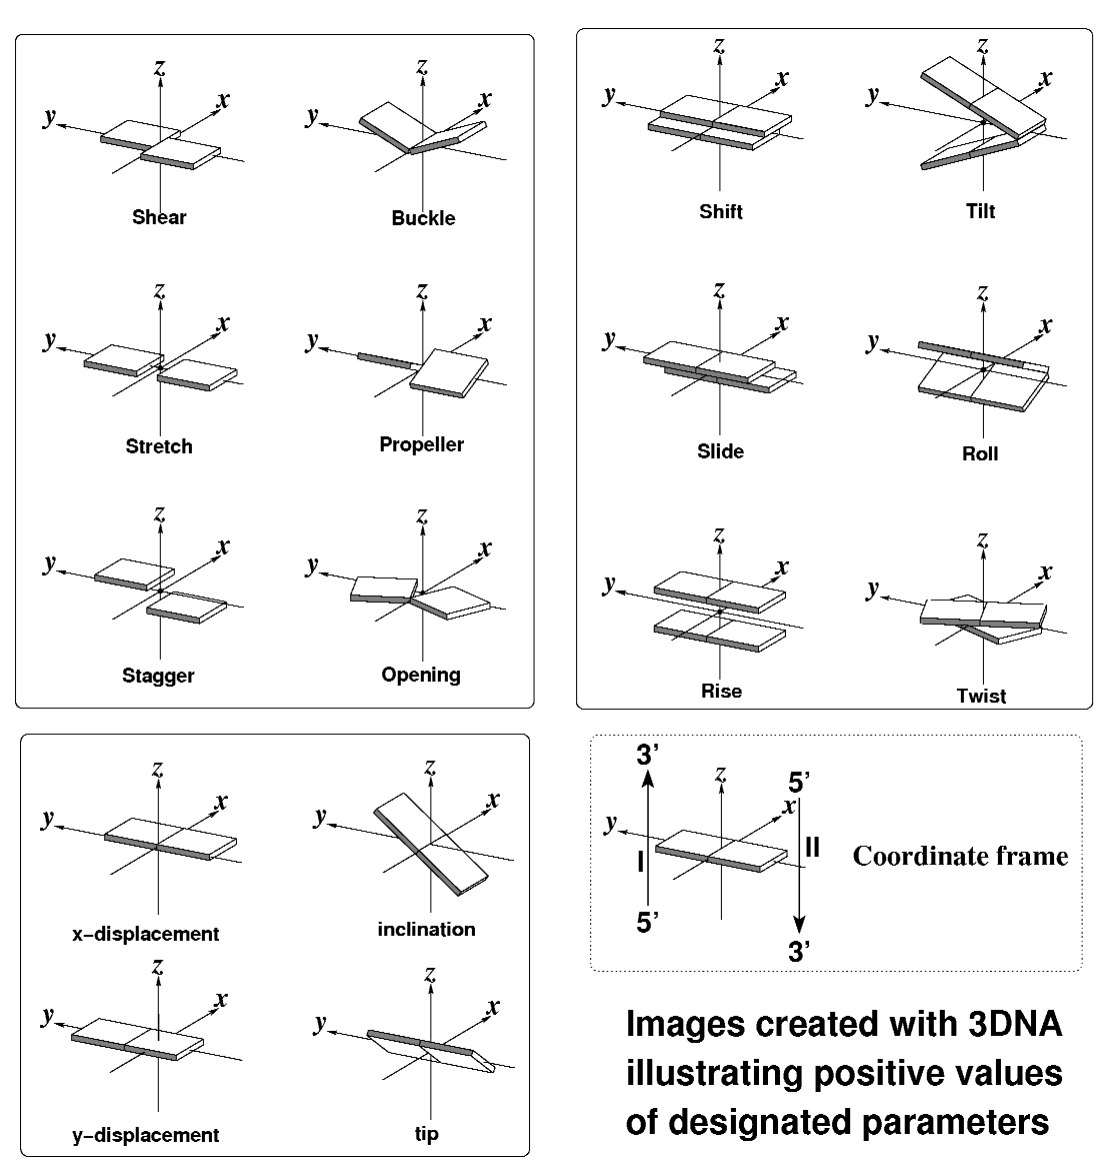
\includegraphics[scale=0.6]{Chapter1/allparam2.png}
\caption{Illustration   of   base-pair   and  base   step   parameters
  \cite{lu2003}.   As seen  in the  upper  right corner  the base  and
  base-pair step parameters correspond  to the three translational and
  three rotational degrees or freedom which describe the geometry of a
  rigid-body. Thus the three  translational degrees of freedom, Shift,
  Slide, and Rise, are expressed  as linear displacements along the x,
  y and  z axis,  and the three  rotational degrees of  freedom, Tilt,
  Roll, and Twist, as angular displacements around x, y, and z.}
\label{fig:allparam}
\end{figure}


%\begin{gather}
%\gamma = \cos^{-1} (\hat{y}_{iII} \cdot \hat{y}_{iI})\\
%bo = \hat{y}_{iII} \times \hat{y}_{iI}\\
%\hat{bo} = \frac {bo}{\sqrt{bo \cdot bo}}\\
%T_{iII}^{'} = R_{bo}(+\frac{\gamma}{2}) T_{iII} \\
%_{iI}^{'} = R_{bo}(-\frac{\gamma}{2}) T_{iI}\\
%r_{mbt} = \frac{(r_{iII} + r_{iI})} {2}\\
%\omega = cos^{-1}(\hat{x}_{iII}^{'} \cdot \hat{x}_{iI}^{'})\\
%(\hat{x}_{iII}^{'} \times \hat{x}_{iI}^{'}) \cdot \hat{y}_{MBT} > 0, \quad then \ \omega > 0\\
%(\hat{x}_{iII}^{'} \times \hat{x}_{iI}^{'}) \cdot \hat{y}_{MBT} < 0, \quad then \ \omega < 0\\
%\phi^{'} = cos^{-1}(\hat{bo} \cdot \hat{x}_{MBT})\\
%(\hat{bo} \times \hat{x}_{MBT}) \cdot \hat{y}_{MBT} > 0, \quad then \ 180 \geq \phi^{'} \geq 0\\
%(\hat{bo} \times \hat{x}_{MBT}) \cdot \hat{y}_{MBT} < 0, \quad then \ -180 \leq \phi^{'} \leq 0\\
%\kappa = \gamma cos (\phi^{'})\\
%\sigma = \gamma sin (\phi^{'})\\
%[S_xS_yS_z]=T_{MBT}(r_{iI} - r_{iII})
%\end{gather}

\section{Local helical parameters}

Local helical parameters are determined using Chasles's theorem, which
states \cite{babcock1994}:
\begin{quote}
``\textit{One can  always transport  a free rigid  body from one  position and
  orientation  to  another  position   and  orientation  by  a  single
  continuous motion along a unique axis of rotation.}''
\end{quote}

\noindent For  the case of  three-dimensional nucleic acid  base steps
what  this means  is  that, instead  of  rotating around  a series  of
reference-frame  centered  axes  and  then translating  along  another
reference-frame centered  axis, one rotates about  and also translates
along   only   one  common   axis,   which   is  not   reference-frame
centered. This allows us to  define the orientation of a local helical
axis (or unique rotational-translational  axis) as a unit vector given
by equation~\ref{eq:helaxis}:

\begin{gather}
\label{eq:helaxis}  
h=\left[ \begin{array}{c}
h_x\\
h_y\\
h_z
\end{array} \right]
\end{gather}
where:
\begin{gather}
h_x = \frac{\tau}{\Omega_h}, \qquad h_y = \frac{\rho}{\Omega_h},
\qquad h_z = \frac{\Omega}{\Omega_h}
\end{gather}

\begin{gather}
\Omega_h = \sqrt{\tau^2 + \rho^2 + \Omega^2}
\end{gather}

The local helical axis can be defined alternatively \cite{bansal1995}
as a cross product:

\begin{gather}
h = (x_2 - x_1) \times (y_2 - y_1)
\end{gather}
where the  $x$ and $y$ refer to  the reference frames on  base pairs 1
and 2.


\bibliography{biblio}



\chapter{Clustering Analysis (CA)}
\label{appendix_a}
\bibliographystyle{nar}
\section{General Methodology}
We considered  each of  the 20 non-A-RNA  type structures as  a vector
composed of  six base step  parameters.  We group these  vectors using
cluster analysis  following an automated process  shown to succesfully
reproduce well  known patterns of  the periodic table from  a selected
set  of variables, such  as, electronegativity,  ionization potential,
and  other elemental  properties  \cite{restrepo2004}.  The  procedure
followed  here  is  an  adaptation   of  how  clustering  is  used  to
re-construct the periodic table classification of the elements.

We start by normalizing the vectors of step parameters,
\begin{gather}
\label{eq:normalization}  
\overline{x}_{jA}=\frac{x_{jA}-x_{jmin}}{x_{jmax}-x_{jmin}}
\end{gather}
where ${x}_{jA}$ is the value  of the step parameter \textit{j} of the
structure A and $x_{jmin}$ and  $x_{jmax}$ are the minimum and maximum
values for a particular step parameter \textit{j} \cite{restrepo2006}.
Then,  using  the  software  package \textsf{R}  \cite{ihaka1996},  we
cluster these vectors into groups.  These groups can be displayed in a
tree  representation,  also called  a  dendrogram,  or  in biology,  a
phylogenetic tree (see Figure~\ref{fig:tree}).

To cluster  these vectors into groups,  it's necessary  to define the
distance between  the vectors. In  this work we used  three distance
definitions.   These distances  are  often referred  to as  Manhattan,
Euclidean  and   maximum  distances.  The  first   two  distances  are
particular cases of what is known as Minkowski's metric:
\begin{gather}
d(X,Y)= \Big( \sum_{i=1}^N |x_i-y_i|^k \Big)^\frac{1}{k}
\end{gather}
where $d(X,Y)$ refers to the distance between two vectors $X$ and $Y$,
where $N$ is  the dimensionality of the vector.  For  the case of step
parameters, $N$ is  six.  In the case where \textit{k}  is equal to 1,
the  definition  corresponds to  the  Manhattan  distance (a  distance
measured by  following along the edges  of blocks). In  the case where
\textit{k} is equal to 2, we have the familiar Euclidean distance. The
remaining distance, that is, the maximum distance, is defined by:
\begin{gather}
d(X,Y) = max |x_{i}-y_{i}|
\end{gather}
where  the  distance  between  vectors  $X$ and  $Y$  is  the  maximum
difference between vector variables.

Yet  another distance  definition used  in  this text,  which is  more
frequently interpreted as an statistical measure of error, is the root
mean square  deviation (RMSD). The  root mean square deviation  can be
seen as a  mean euclidean distance, in the sense  that it's defined as
the square  root of the ratio  between the sum  of squared differences
between vector variables, and the dimensionality of the vectors $N$.

\begin{gather}
RMSD(X,Y)      =     \Big(      \frac{\sum_{i=1}^2     |x_i-y_i|^2}{N}
\Big)^\frac{1}{2} \label{eq:rmsd}
\end{gather}

\noindent Once the  distance is defined, we use  a hierarchical method
to cluster  the space of distances between  base-step parameters.  The
clustering algorithm first finds the two closest vectors (given by one
of  the  distance definitions)  and  groups  them  together.  Then  it
compares the  distance of the elements  in the newly  formed group and
the  elements remaining  to be  grouped, according  to  the particular
clustering method.  For example,  the single linkage clustering method
takes  the  minimum  distance   between  elements  as  the  clustering
criterion.   Such  an  approach  would  (as  all  other  agglomerative
hierarchical methods do), group together the closest vectors given the
distance definition, and then would use the method definition (minimum
distance) to compare the distance of the elements of the group, to the
elements  which  remain  ungrouped,   or  to  the  elements  of  other
groups. As new  groups are formed the process  is repeated following a
hierarchical order,  that is, whatever  distance is smaller  gives the
grouping  criterion.   We   have  used  four  hierarchical  clustering
methods, the description of these methods follows in the next section,
"Hierarchical Methods".

For  every  possible combination  of  clustering  method and  distance
definition we  obtain a dendrogram. The combination  of three distance
definitions and four clustering  methods leads to 12 clustering trees.
These trees are not all exactly  the same but show recurring groups of
conformers.  To find the groups  which are repeated among the trees, a
consensus  analysis  is  performed  using  the  \textsf{clue}  package
\cite{hornik2005} implemented  in \textsf{R}. The  resulting consensus
tree is illustrated in Figure~\ref{fig:eucl_cons}.

\section{Hierarchical methods}
The hierarchical clustering methods used were:

\begin{enumerate}
\item{ \textit{Single linkage  clustering}, where the minimum distance
  between elements of each cluster is taken as clustering criteria.
\begin{gather}
D(X, Y)=min\{d(x_i, y_j): x_i \in X, y_j \in Y \}
\end{gather}
where  $X$ and  $Y$ are  vectors, and  $d(x_i, y_j)$  is  the distance
between cluster elements.  }

\item{  \textit{Complete   linkage  clustering},  where   the  maximum
  distance between cluster elements is the clustering criteria.
\begin{gather}
D(X, Y)=max\{d(x_i, y_j): x_i \in X, y_j \in Y \}
\end{gather} }

\item{ \textit{Average linkage  clustering}, the mean distance between
  elements of each cluster is taken as clustering criteria.
\begin{gather}
D(X, Y)=\frac{1}{N_x  * N_y} \sum_{i=1}^{N_x}  \sum_{j=1}^{N_y} d(x_i,
y_j)
\end{gather}
where  $N_x$  and $N_y$  are  the  number  of elements  in  respective
clusters.  }

\item{ \textit{Centroid linkage clustering}, uses the distance between
  cluster centroids, as clustering criteria.
\begin{gather}
D(X, Y)=d(\overline{x}, \overline{y})\\
\overline{x} = \frac{1}{N_x} \sum_{i=1}^{N_x} x_i\\
\overline{y} = \frac{1}{N_y} \sum_{i=1}^{N_y} y_i
\end{gather} }

\item{ \textit{Ward's  Method}, uses the  error sum of  squares (ESS).
%This Error Sum of Squares might  be the same as the residual sum of
%squares which is important in regression models.
\begin{gather}
D(X,Y)=ESS(XY) -[ESS(X) + ESS(Y)]\\
ESS(X)=  \sum_{i=1}^{N_x} \left|
x_i -\frac{1}{N_x}\sum_{j=1}^{N_x} x_j\right|^2
\end{gather} }
\end{enumerate}

%Yet  another clustering  tecnhique  used  in this  thesis  is that  of
%consensus  clustering. In  our case  we have  only used  one consensus
%clustering     algorithm      known     as     Euclidean     consensus
%clustering.   Euclidean  consensus   clustering  consists   simply  in
%minimizing a function which is  the weighted sum of the absolute value
%of the  squared difference between ultrametrics for  all hierachies or
%partitions which are to be queried for consensus.

%\begin{gather}
%L(U) = \sum_{b} w_{b} \|U-U_{b}\|^{2}\\
%min L(U)
%\end{gather}  

%Where an ultrametric  $U$, refers to a metric  which instead of having
%to comply to  the triangle inequality, it has to  comply to the strong
%triangle inequality:

%\begin{gather}
%d(X,Y) \le max(d(X,Z),d(Y,Z))
%\end{gather}  

As an example lets think of a case where we have five structures. Each
one of  them is descibed by  a bidimensional vector  as illustrated in
Table~\ref{tab:data}.
\begin{table}
\centering
\begin{tabular}[h]{|c|c|c|}
\hline
Structure & Property I & Property II\\
\hline\hline
1  &     1.00  &  5.00 \\
\hline
2  &    -2.00  & 6.00 \\
\hline
3  &      2.00  & -2.00 \\
\hline
4  &     -2.00  & -3.00 \\
\hline
5  &     3.00  &  -4.00 \\
\hline
\end{tabular}
\caption{Example of  structures, considered as  bidimensional vectors,
  to be clustered  using the average linkage method  and the Manhattan
  distance.}
\label{tab:data}
\end{table}

The  first step  is  to chose  a  distance definition.   We chose  the
Manhattan distance.  The  Manhattan distance values between structures
can be displayed in a  lower triangular matrix (usually refered simply
as the distance matrix) as seen in equation~\ref{eq:man}
\begin{gather} 
d(X, Y)=
\begin{vmatrix}
   & 1  &  2   & 3 & 4 & 5 \\
1  & 0  &      &   &   &   \\
2  & 4  &  0   &   &   &   \\
3  & 8  & 12   & 0 &   &   \\
4  & 11 &  9   & 5 & 0 &   \\
5  & 11 & 15   & 3 & 6 & 0 \\
\end{vmatrix}
\label{eq:man}
\end{gather}

Now,  let's  calculate  explicitily  the  Manhattan  distance  between
structures 2 and 3,

\begin{gather}
d(2, 3)= |-2.00 - 6.00| + |2.00 - -2.00| = 12
\end{gather}

Once we have calculated the  distances we pick a clustering method, in
this case,  we will use  the average linkage clustering  method. There
are two hierarchical techiques called agglomerative, or bottom-up, and
divisive, or  top-down. We will use the  agglomerative technique, that
is, going  from the bottom where  no objects are grouped,  to the top,
where all objects  constitute one final group. The  first step is then
to group whatever  structures are closer, that is,  structures 3 and 5
($d(3, 5)=3$). Now  we find the mean distance  between the elements of
this  cluster  and  the  remaining unclustered  structures,  that  is,
structures 1, 2 and 4, we obtain the following mean distances
\begin{gather}
D(\{3,5\}, 1)=\frac{1}{2*1}*(8+11) = 9.5 \\
D(\{3,5\}, 2)=\frac{1}{2*1}*(12+15) = 13.5\\
D(\{3,5\}, 4)=\frac{1}{2*1}*(5+6) = 5.5 \label{eq:dist}
\end{gather}
Since  the distances between  \{3, 5\}  and all  remaining unclustered
vectors is  higher than  the distance between  vectors 1 and  2 ($d(1,
2)=4$) then \{1, 2\} are grouped. The following value, in hierarchical
increasing   order   is   5.5    between   \{3,   5\}   and   4   (see
equation~\ref{eq:dist}), so  we group them. The  next value, following
the lower to higher hierarchy, is 6 ($d(4, 5)=6$), but we have already
grouped 3  with 5, so we have  to keep advancing in  the hierarchy and
we'll find that  the only remaining posibility for  grouping is, group
\{1, 2\} and \{4, 3, 5\},  so we group them together as illustrated in
Figure~\ref{fig:tree}.
\begin{figure}[t]
\centering
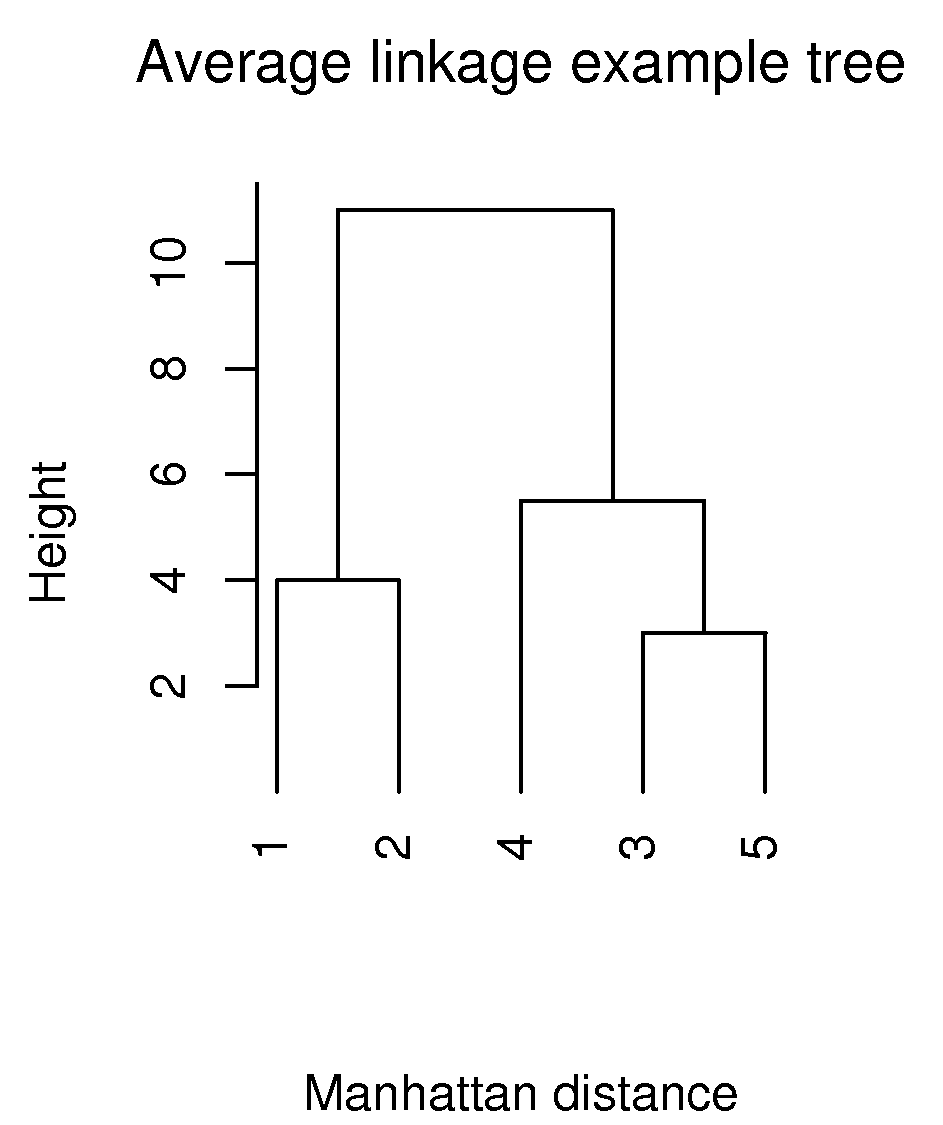
\includegraphics[scale=0.3]{Appendix/appendixtree.png}
\caption{Clustering  tree  for   5  bidimensional  vectors  using  the
  Manhattan  distance definition  and the  average  linkage clustering
  method.}
\label{fig:tree}
\end{figure}

\section{Clustering Validation Techniques}
\label{sec:validation}
The main objective of automated  clustering methods is that of finding
a reduced number of groups which share common characteristics in large
datasets. The main problem with the practical approaches used to solve
this task is that clustering methods do not offer 'a priori' an answer
to the  optimal number  of groups  that a large  dataset can  be split
into. In  our simple example  shown in Figure \ref{fig:tree}  our data
splits into two main groups.  Since this assesment is dependent on the
distances  and clustering methods  used in  particular cases,  then an
emergent necessity is that of  being able to determine the validity of
an   optimal  number   of  clusters   solution.   Such   methods,  not
surprisingly, are  known as clustering validation  techniques, and are
crucial  in the analysis  of the  gigantic amounts  of data  which are
being produced in the  the post-genomic boom of biological information
\cite{handl2005}, having  as a particular  case the one dealt  with in
this thesis.

We have  used the package clValid \cite{brock2008}  which implements a
variety  of  clustering validation  algorithms  using the  programming
language  \textbf{R}  \cite{rcite}.   The  clValid  package  comprises
measures which reflect  the compactness, connectedness, and separation
of cluster partitions. The concept  of compactness of a cluster refers
to the extent of  intra-cluster variation, the conectedness concept is
a more local  concept and means that neighboring  data elements should
belong to the same cluster, and the separation concept quantifies the
degree of separation between individual clusters. An illustration of
this concepts can be seen in Figure \ref{fig:concomsep}.

\begin{figure}
\centering
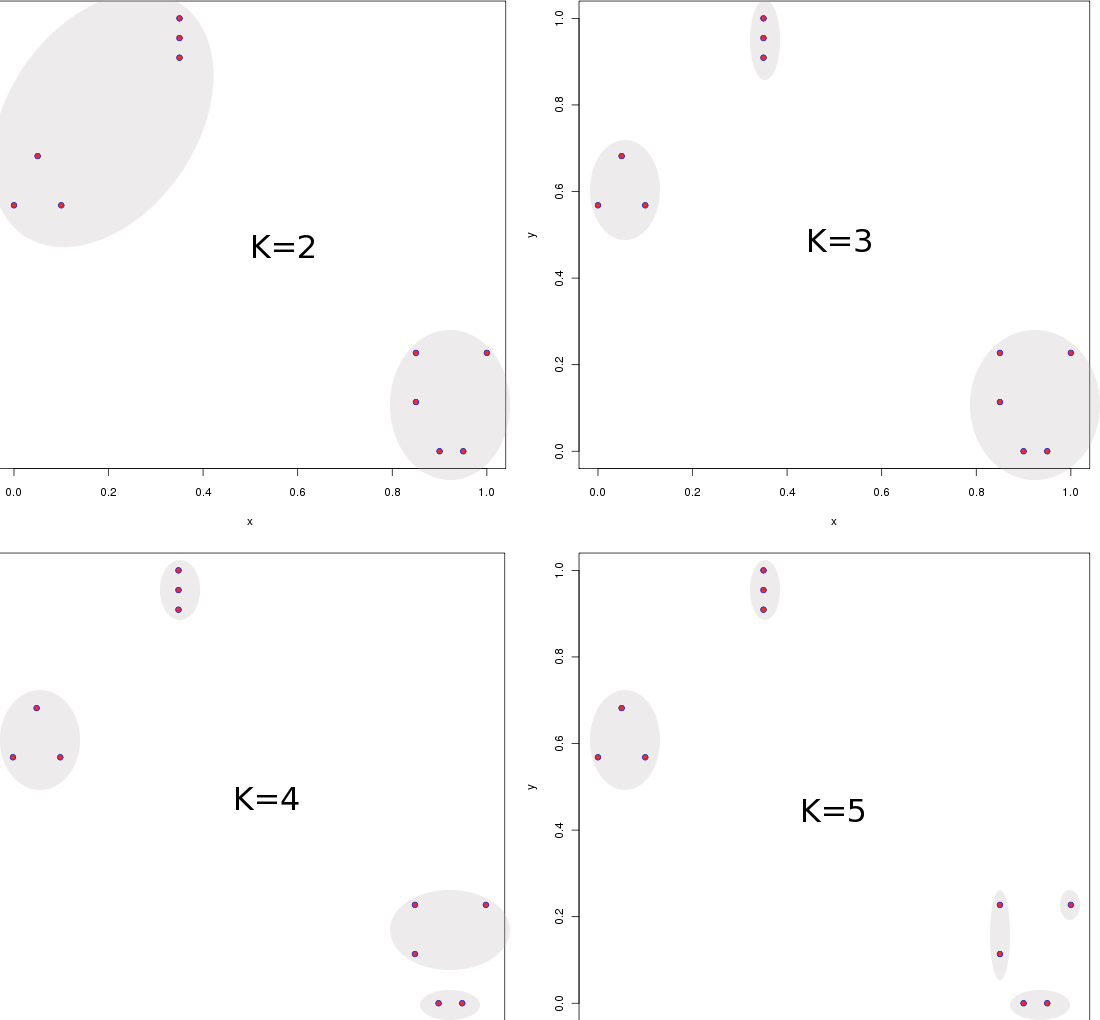
\includegraphics[scale=0.4]{Appendix/consilcom.png}
\caption{We  illustrate in  this figure  the concepts  of compactness,
  connectedness, and separation in a bidimensional example.  In images
  (a)  trough  (d)  we  have  solutions  for  hierarchical  clustering
  considering  $K=[2-5]$ clusters.   For the  case of  three clusters,
  i.e. $K=3$,  we see that compared  to the other  solutions, this one
  stands out as  being composed of more compact  and separated groups,
  this fact would be quantified in  clValid with the asw index and the
  Dunn Index.  For  the two cluster solution in (a) we  see that it is
  clearly more  connected than  all other solutions,  but we  can also
  appreciate that  as we group  data into more  clusters, connectivity
  will be progressively  lost just due to the fact  of dat being split
  apart.}
\label{fig:concomsep}
\end{figure}  

\subsection{Internal Measures}
There are two main types of measures in the clValid package, these are
called internal measures, and stability measures. In general, internal
measures are those which use, exclusively, the dataset, the clustering
partitions,  and intrinsic  information in  the data  to  quantify the
quality of a  clustering result. In clValid three  indices are used to
account for compactness, conectedness and separation, the connectivity
index is used to measure cluster connectedness, and the the silhouette
width  and  Dunn index  combine  measures  of  cluster separation  and
compactness.

\subsubsection{Connectivity Index}
The connectivity index is defined as:
\begin{gather}
Conn(\mathcal{C}) = \sum_{i=1}^{N}\sum_{j=1}^{L} x_{i,nn_{i(j)}}
\end{gather}
Where $nn_{i(j)}$ stands for the $j^{th}$ nearest neighbor (nn) to the
$i^{th}$ observation.  If $i$,  and it's neareast neighbor $nn_{i(j)}$
are in  the same  cluster the term  $x_{i,nn_{i(j)}}$ is zero,  and if
they don't  belong to the  same cluster then  this term is  assigned a
value of $1/j$.  The parameter $L$ resembles a radius, in
the sense that it determines how many nearest neighbors are taken into
account per connectivity weight.
\begin{gather}
x_{i,nn_{i(j)}} =
    \begin{cases}
      0           &  \text{if } i \text{ and } nn_{i(j)} \in C_{k} \\
      \frac{1}{j} &  \text{otherwise.}
    \end{cases}
\end{gather}  
The  connectivity is  defined  for a  particular clustering  partition
$\mathcal{C} =  {C_{1},..., C_{K}}$, that is, for  a particular number
of clusters $K$ where the total number of observations is $N$. 
The connectivity index can give values between zero and $\infty$,
and smaller values mean better connectivity.

\subsubsection{Average Silhouette Width}
The average silhoutte width is the mean of silhoutte values $S(i)$
for $n$ observations.
\begin{gather}
asw = \frac{1}{n} \sum_{i=1}^{n} S(i)
\end{gather}  
The silhoutte value is defined as:
\begin{gather}
\label{eq:silval}  
S(i) = \frac{b_{i}-a_{i}}{\max(a_{i},b_{i})}
\end{gather}
Where $a_{i}$ is the average dissimilarity of observation $i$ to other
observations inside the cluster $i$ belongs to, and
$b_{i}$ is the average dissimilarity of observation $i$ to to
observations outside its own cluster. 
\begin{gather}
a_{i} = \frac{1}{n(C(i))} \sum_{j \in C(i)} d(i,j)\\
b_{i} = \min_{C_{k} \in \mathcal{C}} \sum_{j \in C_{k}}\frac{d(i,j)}{n(C_{k})}
\end{gather}  
The dissimilarity $d(i,j)$ is usually just a distance, for example the
Euclidean or  Manhattan distances, although formally it  does not need
to be  a metric, hence a  dissimilarity.  Notice that  due to equation
\ref{eq:silval}  the  average silhoutte  width  (asw)  can only  have
values    in   the    range   $[-1:1]$.     Kaufman    and   Rousseeuw
\cite{kaufman1990}  suggest  that  acceptable classifications  usually
have an asw value above 0.5  and those with values below 0.2 should be
considered as not  well classified.  Notice in the  lower left plot of
Figure   \ref{fig:internal}  that   all  values   for   validation  of
hierachical clustering for  single-base step-parameters are above 0.5.
The  asw  is  then  an  index  which  quantifies  the  separation  and
compactness of clustering solutions.

\subsubsection{Dunn Index}
The Dunn index is  similar to the asw index in the  sense that it also
quantifies the separation and  compactness of clustering solutions. It
is   an  index  which   measures  the   ratio  between   the  smallest
inter-cluster  distance and  the largest  intra-cluster distance  in a
partitioning.  The index is defined by:
\begin{gather}
D(C) = \min_{C_{k} \in C} \left(  \frac{\min_{C_{l} \in C}
  d(C_{k},C_{l})}{\max_{C_{m} \in C} diam(C_{m})} \right)
\end{gather}
Where $\min_{C_{l \in C}} d(C_{k},C_{l})$ is the minimum inter-cluster
distance,  and  $\max_{C_{m}  \in   C}  diam(C_{m})$  is  the  maximum
intra-cluster distance.   The Dunn index can have  values between zero
and $infty$, and a higher  value means a better cluster separation and
compactness.

\subsection{Stability Measures}
Stability  measures are  a  special type  of  internal measures  which
evaluate the consistency of a clustering result by comparing clustered
groups after sequential removal  of a column of data \cite{datta2003}.
In  the following  definitions  $N$  stands for  the  total number  of
datapoints  (rows of data)  and $M$  is the  total number  of columns,
dimensions  in the  data.  The  dimensions in  datapoints  usually are
taken as  a collection of samples  or time points.  These measures are
specially suited  for highly correlated  data as is commonly  the case
for  high-throughput genomic  data,  like micro-arrays.  In the  cases
shown here an average is taken over the combined space of the full
data and reduced data sets.

\subsubsection{Average Proportion of Non-overlap (APN)}
APN is a measure of the  proportion of datapoints which are not placed
in the  same cluster when a  comparison is made between  the full data
clustering,  and that  done with  one column  of data  removed  and is
defined as:
\begin{gather}
APN(\mathcal{C}) - \frac{1}{MN} \sum_{i=1}^{N}\sum_{l=1}^{M} \left( 1
- \frac{n(C^{i,j} \cap C^{i,0})}{n(C^{i,0})} \right)
\end{gather}  
Where $C^{i,0}$ is the cluster which contains the datapoint $i$ in the
full dataset, and $C^{i,l}$ is the cluster which contains point $i$ in
the  reduced dimensionality  dataset, where  the column  $l$  has been
removed.  The  value of APN is  ranges between $[0-1]$  and is optimal
for values closer to zero.


\subsubsection{Average Distance (AD)}
The  AD  measure  computes   the  distance  between  datapoints  in  a
particular cluster of the full  dimensional dataset and that where one
column, or dimension has been taken off.
\begin{gather}
AD(\mathcal{C})=\frac{1}{MN}       \sum_{i=1}^{N}\sum_{l=1}^{M}      -
\frac{1}{n(C^{i,0})n(C^{i,l})}  \left[  \sum_{i  \in  C^{i,0},  j  \in
    C^{i,l}} d(i,j) \right]
\end{gather}
Where $d(i,j)$ is the distance between points $i$ in the full dimensional
dataset and points $j$ in the reduced dimension dataset.
The values of AD range  between $[0-\infty]$ and are optimal when they
come closer to zero.

\subsubsection{Average Distance Between Means (ADM)}
The ADM  score measures  the distance between  the mean  of datapoints
values within  a cluster  with the full  number of dimensions  and the
mean of datapoints  of the same cluster when  reduced by one dimension
or column.
\begin{gather}
ADM(\mathcal{C})= \frac{1}{MN} \sum_{i=1}^{N} \sum_{l=1}^{M}
d(\bar{x}_{C^{i,l}}, \bar{x}_{C^{i,0}})
\end{gather}  
Where  $\bar{x}_{C^{i,0}}$ is  the  mean value  of  datapoints in  the
cluster   which  contains  point   $i$  in   the  full   dataset,  and
$\bar{x}_{C^{i,l}}$  is the mean  value of  datapoints in  the cluster
containing point $i$ with column $l$ removed.  The values of ADM range
between $[0-\infty]$  and are  also as AD  and APN optimal  the closer
they are to zero.

%\newline
%Distance can be defined by Minkowski's metric:
%\begin{gather}
%d(X,Y)= \Big( \sum_{i=1}^N |x_i-y_i|^k \Big)^\frac{1}{k}
%\end{gather}
%In the particular case when $k=1$ we have the definition of the
%Manhattan or taxi-cab distance and when $k=2$ it's the familiar
%Euclidean distance.

%Finally, we can also define a maximum distance as the maximum
%difference between vectors variables.
%\begin{gather}
%d(X,Y) = max |x_{i}-y_{i}|
%\end{gather}

\bibliography{biblio}



%\chapter{Dimension Reduction}
\label{pca}
\bibliographystyle{nar}
\section{Principal Component Analysis}
Given  a set  of data  it's important  to check  before analysis  if the
dimensions of such  set can be reduced. A very  common method to check
this is called Principal Component Analysis (PCA).

The PCA  method can be defined  in a strictly mathematical way as the
method which; finds the Principal  Components (PCs) of  a dataset by
doing  "an orthogonal  linear  transformation of  a  set of  variables
optimizing certain algebraic criterion" \cite{jolliffe2002}.

\begin{gather}
  \mathbf{y} = \mathbf{T} \mathbf{x}
\end{gather}

Where $\mathbf{T}$ is an orthogonal linear transformation matrix of
dimension $k$ by $n$, $\mathbf{x}$ is the "original" data matrix of
dimension $n$ by $m$, and by definition of the matrix product
$\mathbf{y}$ is a matrix of dimension $k$ by $m$.

From the linear tranformation expression it's clear that if $k=m$ then
the transformation matrix is just a rotation matrix, and in the case
where $k<m$ then the transformation matrix is also reducing the
dimension of the "original" data.

One common algorithm to find such transformation ($\mathbf{T}$) is the
following: 

\begin{enumerate}
\item{Substract the mean from the data matrix $\mathbf{x}$.
\begin{equation}
\mathbf{\Omega} = \mathbf{x} - \mathbf{\bar{x}_{m}}
\end{equation}
}
\item{Find the covariance matrix for $\mathbf{\Omega}$.
\begin{equation}
\mathbf{\Sigma} = \frac{\mathbf{\Omega}^{-1} \mathbf{\Omega}}{(1-n)}
\end{equation}  
}  
\item{Diagonalize the covariance matrix $\mathbf{\Sigma}$.
\begin{equation}
\mathbf{T}^{\mathrm{T}} \mathbf{\Sigma} \mathbf{T} = \mathbf{\Lambda}
\end{equation}  
}  
\item{Organize $\mathbf{T}$ from the highest to lowest eigenvalues in
$\mathbf{\Lambda}$.}
\end{enumerate}  

Obtaining the eigenvalues and eigenvectors of $\mathbf{\Sigma}$ means
that we have found our transformation matrix $\mathbf{T}$, which can
be used to either rotate the original data space to an orthonormal
one, or to reduce the dimensionality of the data space by choosing
$k<m$, depending on the weight of the eigenvectors in
$\mathbf{\Lambda}$. The $k$ rows of $\mathbf{y}$ are named Principal
Components.

There is a large amount of bibliography which refers to the statistics
of Principal Components Analysis, and to sofistications which are not
included in this brief appendix. An interested reader can find great
help in the following web addresses:\\
\url{http://www-stat.wharton.upenn.edu/~buja/script-Buja-CU-2009-06-pca.R}\\
\url{http://www.snl.salk.edu/~shlens/pca.pdf}\\
\url{http://www.cse.unr.edu/~bebis/MathMethods/PCA/lecture.pdf}

\bibliography{biblio}



\part{Introduction}
\label{appendix4a}
\bibliographystyle{nar}
Nucleic Acids and other polymers can be understood as mechanical
objects \cite{marko2003, nelson2004} and therefore engineering
approaches can be used for their understanding. Usually the methods
followed by the engineering approach neglect details which can be
intrinsic to the local chemistry of the subunits which make up the
polymer. Dr. Olson and collaborators have suggested a formal approach
refered to as the "realistic" model \cite{olson1993}, which takes into account details
at the sequence level for the case of nucleic acids. This model is
dependent on a knowledge-based approach, where, force constant analogs
are derived from crystallographic data using a so called covariation,
or go model \cite{go1974}.





Continuous vs discrete models.





The previous is not exactly true, we are using a completely physical
model, the only thing is that we are linking different parts, that is,
we are assuming that the connected parts have springs with different
constants, that't it. It is as if we were connecting pieces of steel,
with pieces of rubber, and pieces of wood, let's say.

Global properties of DNA as a polymer do not depend so much in
structural detail, but local properties are definetely described at
the chemical-molecular-atomic level.

The realistic model, in a way, bridges the gap between non-sequence
dependent elasticity theory models, and sequence dependent
molecular-bond (can be virtual-bond) based models.


that is, like rigid rods, say a steel bar, or like flexible rods, say
a rubber tube.

The "realistic model" is general an can be simplified to other models,
for example to the freely rotating model, just by making the twisting
constant zero, that is, the polymer will not be elastic when twisted.
when stretching constan 



To quantify the rigidity of a polymer

Biopolymers can be either rigid or flexible. 

They can be classified  according to whether their persistence length ($a$)
is greater, smaller, or similar to the contour length ($L$) of the polymer.

\begin{table}[htbp]
\begin{center}  
\begin{tabular}{c|c|c}
\hline
Model Type      & Polymer Characteristic & $a$ to $L$ relation\\ \hline
Rigid Rod       & Rigid          &        $a >> L$   \\
Gaussian chain  & Flexible       &        $a << L$   \\
Worm-like chain & Semi-flexible  &    $a \approx L$ \\
\hline
\end{tabular}
\end{center}
\end{table}

Worm-like-chain = Porod-Kratky = Freely Rotating Chain in limit l=0
and n=infinity
\\

Rigid biopolymers:
actin, microtubules
\\

Flexible biopolymers:
\\

Semi-flexible biopolymers:
High force extension DNA.
\\

If the persistence length is of the same order of the length of the
polymer, then the polymer is classified as  semi-flexible


\begin{table}[htbp]
\begin{center}  
\begin{tabular}{c|c}
\hline
Polymer       & $a$ (nm)   \\ \hline
$\alpha$-helix & 80-100\\
coiled-coil & 150-300\\
Ideal DNA  &  51  \\
Ideal RNA & 70-80 \\
\hline
\end{tabular}
\caption{Persistence lengths for some biopolymers with filament structures.}
\end{center}
\end{table}

Think about the "energy" based perspective of Nicolas, and the
stochastic based perspective of Flory and others.




\section{Persistence Lenght Definitions}

``\textbf{Bend-persistence length}:\\ 
A length scale beyond which the elastic cost of bending is totally
negligible''

``In a randomly shaken rod any particular point in the rod will be
pointing in a random direction, but nearby points will be pointing in
roughly the same direction, that is, this nearby points are
persistent. Points farther away than the bend-persistence length are
said to be uncorrelated.''

there is also twist-persistence length.
that is, there is, a rubber rod not only resists bending but also twisting.

"length at which the orientation of the sequential bonds which make
up a polymer chain, stop being correlated. That is, if you have just
two bonds, they will be correlated, which is the case in most
molecules, but, in polymers, you have a long chain of sequential
bonds. At some length, bonds will become uncorreleted, but up to that
lenght they were correlated, this is what is meant by persistence
length, and, in this context it's obvious that is an exclusive
property of polymers."

"the average sum of the projections of all bonds $ j \geq i$  in an 
indefinetely long chain."


\begin{table}[htbp]
\begin{center}
\begin{tabular}{|l|l|l|l|}
\hline 
polymer & lp(\AA) & T (Kelvin) & Phase \\ \hline
DNA     & 500     &  273       & water \\ \hline
\end{tabular}
\end{center}
\end{table}



\section{end-to-end}
The end-to-end vector  $r$ is the vector which connects  the ends of a 
polymer chain.  It  can be defined  as the sum  of the vectors connecting the
monomer units in a chain. These connecting vectors are sometimes called
virtual  bond vectors $l$.  

From  the end-to-end  vector  the quantity
which is usually of interest is it's magnitude.

\begin{gather}
\label{eq:end2end}
r = \sum_{i=1}^{n} l_{i}\\
r^2 = r \cdot r = \sum_{i,j}l_{i} \cdot l_{j}
\end{gather}
Equation \ref{eq:end2end}, can also be written:
\begin{gather}
r^2 = \sum_{i}l_{i}^{2} + 2 \sum_{i\neq j} l_{i} \cdot l_{j}
\end{gather}  

To  describe a  polymer  it's  necessary to  think  about the  various
conformations it can adopt  due to its flexibility, therefore, it
is important  to think of polymer  related quantities in  terms of the
average of their possible conformations. For the end-to-end vector the
average of  its values  is denoted  as $<r>$, and  the average  of its
norm, also called the second moment of the end-to-end distribution, is
denoted by $<r^2>$:
\begin{gather}
\label{eq:secmom}  
<r^2>=\sum_{i}<l_{i}^2> + 2\sum_{i<j}<l_{i} \cdot l_{j}>
\end{gather}  

When there is no correlation between succesive bonds we can write:

\begin{gather}
\label{eq:nocorr}
<l_{i} \cdot l_{j}> = 0
\end{gather}

And equation \ref{eq:secmom} reduces to having only the bond self
correlation term:

\begin{gather}
<r^2> = \sum_{i}<l_{i}^2> = n<l^2>
\end{gather}  

This equation is used to describe a so-called freely-jointed chain.


\section{Models}

Nelson in book says:

\begin{gather}
dE={1}{2}\kappa_{B}T[A\beta^2+Bu^2+C\omega^2+2Du\omega]ds
\end{gather}  

A$\kappa \beta$ T = Bend stiffness
B$\kappa \beta$ T = Stretch stiffness
C$\kappa \beta$ T = Twist stiffness
D$\kappa \beta$ T = Twist-stretch coupling

If only the bend stiffness survives then the model is called an
inextensible model, also Porod-Kratky, or WLC.

\subsection{Kuhn - Freely Jointed Chain (FJC)}

\subsection{Porod-Kratky - Worm Like Chain (WLC)}

\subsection{Olson - Realistic}

The Hamiltonian for a \cite{czapla2009}





\section{Suggested Reads}

From Equilibrium Statistics of Plischke and Bergersen they suggest to
read:
Des Cloiseaoux and Janik ()
Rubinstein and Colby (Polymer Physics)
\bibliography{biblio}

\supplement
%\makeatother 
\chapter{Figure Supplements}
\label{supplements}
\bibliographystyle{nar}
\section{Supplement Figures for Chapter 2}
\begin{figure}[ht]
\centering
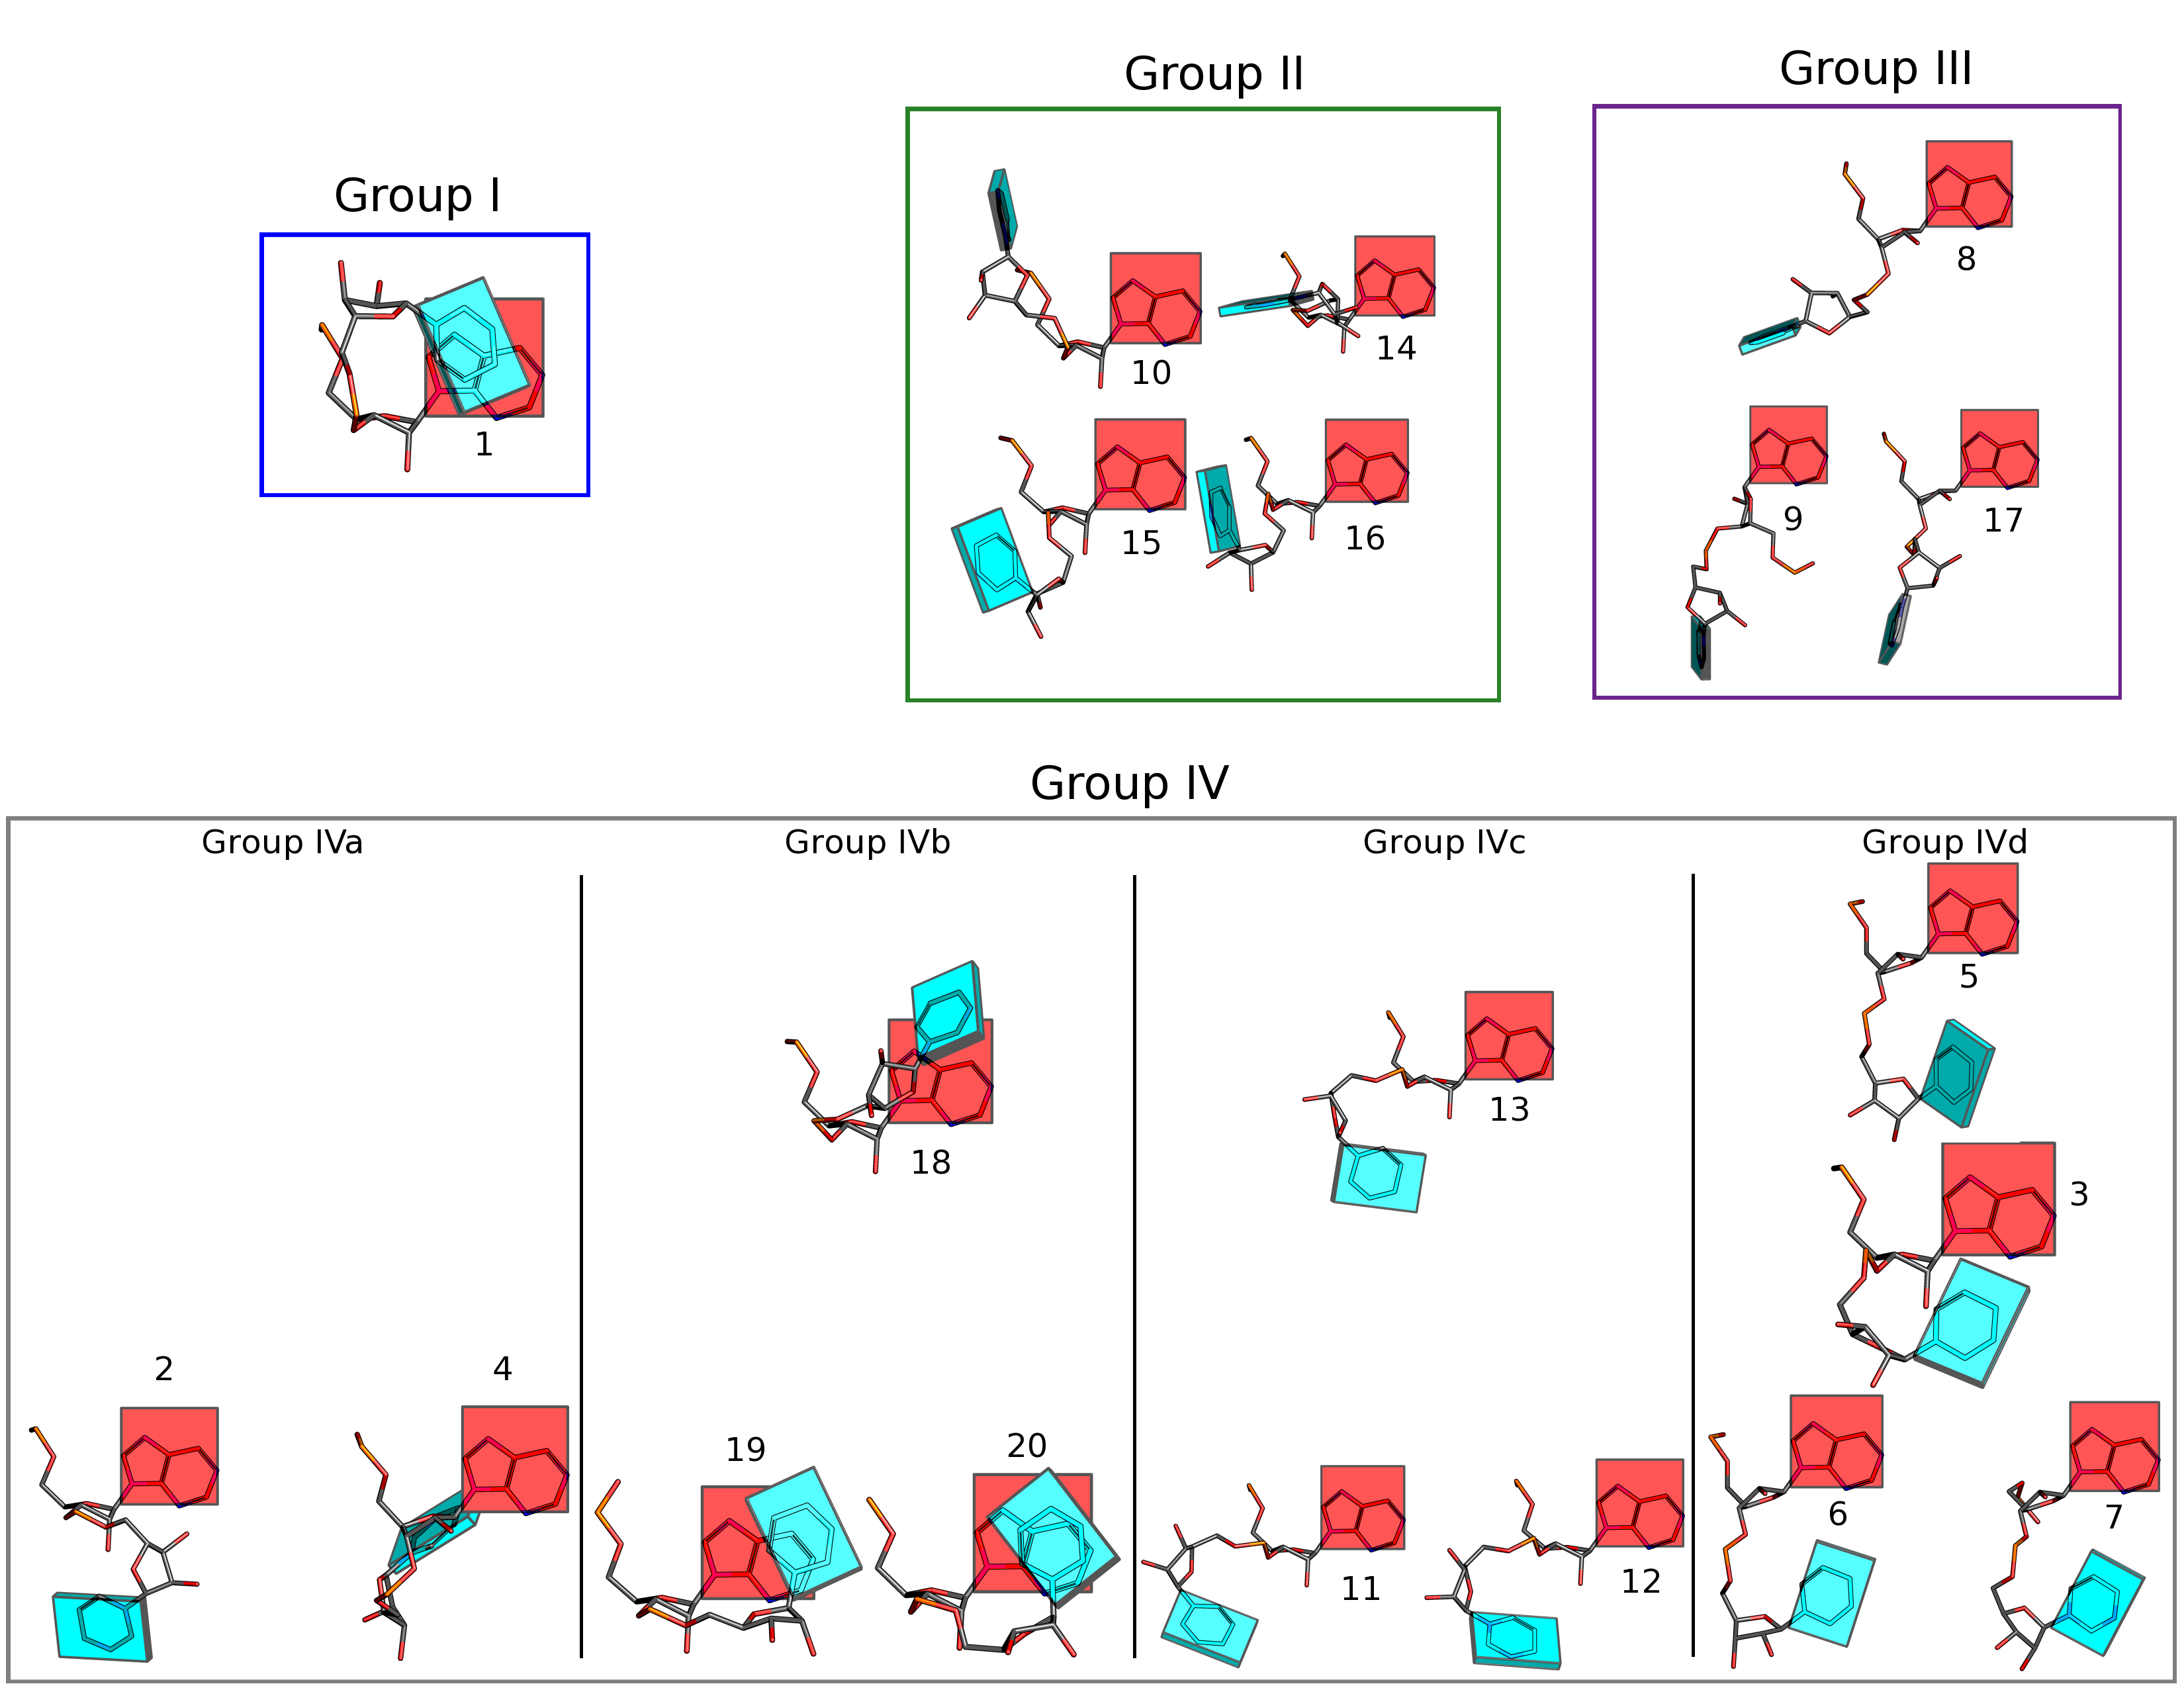
\includegraphics[angle=90, scale=0.4]{Supplement/collage2.png}
\caption{Non A-RNA Type base steps centered on the standard reference
  frame of Adenine. Top view with the Minor Groove side of Adenine
  pointing down the page and the Major Groove pointing up.}
\label{fig:steps2}
\end{figure}

\begin{figure}[t]
\centering
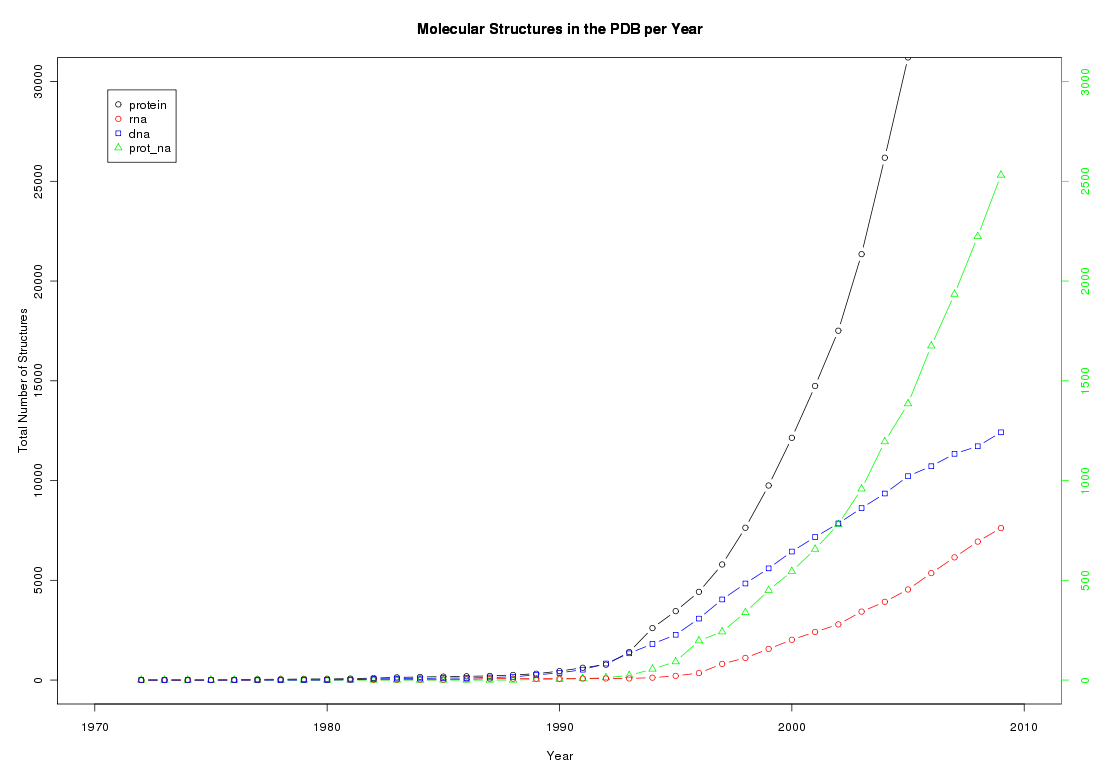
\includegraphics[angle=90, scale=0.5]{Supplement/allmolecules_per_year.png}
\caption{The total number of structures available in the pdb up to the
end of year 2009. The scale of the axis in the left (in black), is ten
times that in the right (in green). The black y-axis sets the scale
for the number of protein structures available in the PDB up to the
end of the year 2009. The green y-axis sets the scale for the number
of molecular structures containing, rna only (in red), dna only (in
blue), and protein plus nucleic acid (in green).
One can clearly see that the total number of protein, rna, and protein
plus nucleic acid structures is growing exponentially. It is also
clear that the number of DNA structures is perhaps tending toward a
constant number, that is, it might not be growing. It is also
interesting to see how the number of RNA structures really lifts off in the
middle of the nineties, whereas for DNA the growth started earlier and
is settling down.}
\label{fig:allpolypdb}
\end{figure}

\bibliography{biblio}



%\chapter{Index}
\printindex*

%\printindex
\makeatletter
\begin{vita}
\heading{Mauricio Esguerra} \vspace{15pt}
% Colleges attended, with dates, subjects, degrees
\begin{descriptionlist}{xxxxx-xxxxx} %reverse chronological order
\item[{\bf La Mala Educacion}] \mbox{}
\item[1991] High School Diploma from Gimnasio Moderno, Bogota, Colombia.
\item[2000] B. Sc. in Chemistry from Universidad Nacional de Colombia
\item[2010] Ph. D. in Chemistry and Chemical Biology, Rutgers University
\end{descriptionlist}
\medskip
\begin{descriptionlist}{xxxxx-xxxxx} %positions held since BS degree
\item[{\bf Professional Experience}] \mbox{}
\item[2003-2009] Teaching assistant, Department of Chemistry and
  Chemical Biology, Rutgers University
\end{descriptionlist}
\medskip
\begin{descriptionlist}{xxxxx-xxxxx} %positions held since BS degree
\item[{\bf Publications}] \mbox{}
\item[2009] W. K. Olson, M. Esguerra, Y. Xin, X-J. Lu, Methods
\end{descriptionlist}

\end{vita} 




\end{document}



%%%%%%%%%%%%%%%%%%%%%%%%%%%%%%%%%%%%%%%%%%%%%%%%%%%
% Compilation Instructions:
%
% latex main
% bibtex main
% bibtex Chapter1/chapter1
% bibtex Chapter2/chapter2
% makeindex main
% latex main
%%%%%%%%%%%%%%%%%%%%%%%%%%%%%%%%%%%%%%%%%%%%%%%%%%%

